\documentclass[a4paper,12pt,openright,twoside]{book}  



%Paquetes
\usepackage[utf8]{inputenc}
\usepackage[spanish]{babel}
\usepackage{graphicx} 
\usepackage{array}
\usepackage{wrapfig}   
\usepackage[scriptsize]{caption} 
\usepackage{amsmath} 
\usepackage{amsthm}  
\usepackage{float}   
\usepackage{lastpage}
\usepackage{pdfpages}
\usepackage{url}
% Package rotating -> Para poder girar las tablas y dibujarlas a lo largo
% del folio en vez de a lo ancho.
\usepackage{rotating}
% Packages multicol y multirow, para manejar tablas de filas y columnas múltiples.
\usepackage{multicol}
\usepackage{multirow}
\usepackage{colortbl}
%Para codigo maquina
\usepackage{listings}
%Para hypervínculos en el indice
\usepackage[hidelinks]{hyperref}
\usepackage{pdfpages}
\usepackage{lscape}
\usepackage{eurosym}
\usepackage{listings}
\usepackage{xcolor}

\usepackage{tabularx}
\usepackage{booktabs}
\usepackage{longtable}

\usepackage{array}

\lstdefinestyle{sharpc}{language=[Sharp]C}

\usepackage{appendix}

\usepackage{epstopdf} 
\usepackage{subcaption}
%Renombramientos


\usepackage{enumitem}
\usepackage{tikz}
\newcommand*\circled[1]{\tikz[baseline=(c.base)]{
    \node[shape=circle,fill=black,text=white,inner sep=1.2pt,
          font=\footnotesize\bfseries] (c) {#1};}}

\renewcommand{\contentsname}{Índice de contenido}
\renewcommand{\chaptername}{Capítulo}            
\renewcommand{\bibname}{References} 
\renewcommand{\listfigurename}{Índice de figuras}
\renewcommand{\listtablename}{Índice de tablas}
\renewcommand{\figurename}{Figura}
\renewcommand{\tablename}{Tabla}
\addto\captionsspanish{\renewcommand{\appendixname}{Anexo}}
%\renewcommand{\appendixname}{Anexo}
\renewcommand{\appendixtocname}{Anexos}
\renewcommand{\appendixpagename}{Anexos}
\renewcommand{\lstlistingname}{Listado}

\newcolumntype{C}[1]{>{\centering\arraybackslash}m{#1}}

\providecommand{\keywords}[1]{\textbf{\textit{Keywords---}} #1}

%\setcounter{secnumdepth}{4}
%\setcounter{tocdepth}{4}

%Configuración páginas

%----------Espaciado y ajuste de márgenes----------
\usepackage{setspace}
\onehalfspacing
\setlength{\textwidth}{15cm}
\setlength{\textheight}{22cm}
\setlength\oddsidemargin{1cm}
\setlength\evensidemargin{0cm}
\setlength{\headheight}{14.5pt}
% Personalizamos la separación entre párrafos...
\parskip=6pt

%-------------------------------------------------


% Para evitar lineas huérfanas
\widowpenalty=10000
\clubpenalty=10000


%-------------------Encabezado de página------------------
\usepackage{fancyhdr}
\pagestyle{fancy}
\fancyhf{}
%La seccion (\rightmark) va a aparecer en:
	%Páginas impares: a la izquierda.
\fancyhead[LO]{\slshape \bfseries \nouppercase \rightmark}
%El capítulo (\leftmark) va a aparecer en:	
	%Páginas pares: a la derecha.
\fancyhead[RE]{\slshape \bfseries \nouppercase \leftmark}
%El número de página va a aparecer en:
	%Páginas pares: izquierda.
	%Páginas impares: derecha.
\fancyhead[RO,LE]{\bfseries \thepage}

%----------------------------------------------------------


%\pretolerance=10000 
%\tolerance=3000     
%\setlength{\parskip}{\baselineskip} 


\begin{document}

\pagestyle{empty}

\begin{center}
	\newcommand{\HRule}{\rule{\linewidth}{0.7mm}}
	\begin{minipage}{0.48\textwidth} 
		\begin{flushleft}
			
\includegraphics[height=3cm]{imagenes/logouex}\\[2.5cm]
		\end{flushleft}
	\end{minipage}
	\begin{minipage}{0.48\textwidth} 
		\begin{flushright}
			
\includegraphics[height=3cm]{imagenes/logocum}\\[2.5cm]
		\end{flushright}
	\end{minipage}	

	\vspace*{2cm}
	\textsc{\large Universidad de Extremadura}\\[0.5cm]
	\textsc{\large Centro Universitario de Mérida}\\[1.3cm]
	\textsc{\LARGE Grado en Ingeniería Telemática en Telecomunicación}\\[1.3cm]
	\textsc{\huge Trabajo Fin de Grado}\\[2cm]
	%{ \large Diseño de metaheurísticas especializadas para la optimización de cadenas de servicios en redes 5G}\\
	\textsc{\LARGE Diseño e implementación de un protocolo de red de área local sobre tecnología LoRa para redes privadas orientadas a IoT}\\[2.5 cm]
	
		%\rule{\linewidth}{0.2 mm} \\[2.5 cm]
	\textsc{\large Javier Conejero Rodríguez}
	\vspace{2cm} 
	\vfill
	Mérida, Noviembre de 2026
\end{center}

\cleardoublepage
\pagestyle{empty}

\begin{center}
	\newcommand{\HRule}{\rule{\linewidth}{0.7mm}}
	\begin{minipage}{0.48\textwidth} 
		\begin{flushleft}
			
\includegraphics[height=3cm]{imagenes/logouex}\\[2.5cm]
		\end{flushleft}
	\end{minipage}
	\begin{minipage}{0.48\textwidth} 
		\begin{flushright}
			
\includegraphics[height=3cm]{imagenes/logocum}\\[2.5cm]
		\end{flushright}
	\end{minipage}	
	
	\vspace*{2cm}
	\textsc{\large Universidad de Extremadura}\\[0.5cm]
	\textsc{\large Centro Universitario de Mérida}\\[1.3cm]
	\textsc{\LARGE Grado en Ingeniería Telemática en Telecomunicación}\\[1.3cm]
	\textsc{\huge Trabajo Fin de Grado}\\[2cm]
	%{ \large Diseño de metaheurísticas especializadas para la optimización de cadenas de servicios en redes 5G}\\
	\textsc{\LARGE Diseño e implementación de un protocolo de red de área local sobre tecnología LoRa para redes privadas orientadas a IoT}\\[2.5 cm]
\end{center}

\begin{flushleft}
	\begin{tabular}{ll}
		% Nombre del alumno.
		\large{\textbf{Autor:}}
		\large{Javier Conejero Rodríguez} \\
		\large{\textbf{Fdo:}} & \\
		\\
		\\
		\\
		% Nombre del director/tutor del proyecto.
		\large{\textbf{Tutor:}}
        \large{Pedro José Pardo Fernández} \\
        \large{\textbf{  Fdo:}}\\
        \\
        \\
        \\
        \large{\textbf{Tutor:}}
        \large{Francisco Díaz Barrancas} \\
        \large{\textbf{  Fdo:}}\\
	\end{tabular}
\end{flushleft}
\cleardoublepage

\pagestyle{plain}
\pagenumbering{Roman} % para comenzar la numeración de paginas en números romanos

\chapter*{Agradecimientos}

¡Al fin cierro mi etapa como estudiante universitario!

Quería agredecer a mi tutor, Pedro, todo el apoyo brindado durante la realización de este trabajo. Sin su ambición este proyecto no habría sido posible y, de primeras, jamás me hubiera lanzado a trabajar a tan bajo nivel diseñando un protocolo dede cero.

Este trabajo ha supuesto un reto para mi, no por la complejidad del contenido en sí mismo, sino por la dificultad que conlleva trabajar con materias tan diferenciadas. 

Gracias también a ti, Sofía. Desde que estás en mi vida solo me han pasado cosas buenas y las que no han sido buenas, han sido menos malas. Eres capaz de sacar lo mejor de mí y eso no tiene precio. Siempre estaré ahí, para apoyarte y ayudarte, al igual que tú haces conmigo.   
\cleardoublepage

\renewcommand{\keywords}{{\itshape \bfseries Palabras clave - }}
\chapter*{Resumen} 
Las tecnologías LPWAN, y en particular LoRa, permiten establecer comunicaciones inalámbricas de largo alcance con un consumo reducido, lo que las convierte en una alternativa de interés para aplicaciones IoT. Sin embargo, LoRaWAN, el protocolo más extendido sobre LoRa, está orientado a despliegues de gran escala y presenta limitaciones para aplicaciones locales que requieren comunicaciones bidireccionales y baja latencia. Este Trabajo de Fin de Grado presenta LoRaLAN, un protocolo de comunicación de área local diseñado directamente sobre la capa física LoRa, y su aplicación a un sistema de registro de asistencia docente mediante tarjetas NFC y monitorización de aulas.

LoRaLAN emplea una topología en estrella y combina un mecanismo de sondeo periódico para el tráfico rutinario con la transmisión asíncrona de eventos urgentes mediante detección de actividad del canal (CAD). También incorpora mecanismos de direccionamiento, control de acceso al medio y protección de los mensajes mediante cifrado y autenticación. Su implementación se ha desarrollado como una biblioteca independiente de la plataforma, ejecutable tanto en plataformas ESP32, Raspberry Pi como en un simulador de PC. La evaluación combina la caracterización del entorno radioeléctrico mediante radio definida por software (SDR), experimentos sobre un canal simulado y validación funcional sobre el hardware.


\keywords{LoRa, LoRaLAN, LPWAN, IoT, Protocolo MAC, Sondeo, CAD, AES, CMAC, ESP32, Simulación, NFC, Control de asistencia.}
\cleardoublepage

\renewcommand{\keywords}{{\itshape \bfseries Keywords - }}
\chapter*{Abstract}


LPWAN technologies, particularly LoRa, enable long-range wireless communications with low power consumption, making them an attractive option for IoT applications. However, LoRaWAN, their most widely adopted protocol, is designed for large-scale deployments and presents limitations for local applications requiring bidirectional communication and low latency. This Final Degree Thesis presents LoRaLAN, a local area network protocol designed directly on top of the LoRa physical layer, and its application to a teacher attendance system based on NFC cards and classroom monitoring.

LoRaLAN employs a star topology and combines a periodic polling mechanism for routine traffic with asynchronous transmission of urgent events using Channel Activity Detection (CAD). It also incorporates addressing, medium access control, and message protection mechanisms based on encryption and authentication. Its implementation is provided as a platform-independent library, executable on both ESP32 and Raspberry Pi platforms, as well as in a PC-based simulator. The evaluation combines radio environment characterization using software-defined radio (SDR), experiments over a simulated channel, and functional validation on the hardware.

\keywords{LoRa, LoRaLAN, LPWAN, IoT, wireless communication protocols, NFC, access control, software-defined radio.}
\cleardoublepage

\pagestyle{plain}
\tableofcontents

\addcontentsline{toc}{chapter}{Índice de figuras}
\listoffigures

\cleardoublepage
%\addcontentsline{toc}{chapter}{Índice de tablas}
%\listoftables
%\cleardoublepage

%\pagestyle{fancy} 
\pagenumbering{arabic}

% CAPÍTULOS -----------------------------------
\chapter{Introducción}\label{chap:1}

\section{Antecedentes y Contextualización}

Internet de las Cosas (IoT, \textit{Internet of Things}) ha experimentado en la última década un crecimiento sostenido que ha transformado la forma en la que se monitorizan y controlan los entornos físicos. Se estima que el número de dispositivos conectados superará ampliamente las decenas de miles de millones durante esta década~\cite{chaudhari2020lpwan}.  

Se denomina IoT a la red de objetos físicos conectados a internet mediante software, sensores y otras tecnologías que son capaces de recopilar e intercambiar datos, facilitando la comunicación y la automatización. IoT abarca objetos cotidianos como electrodomésticos, vehículos e incluso ropa. Esta interconexión permite el monitoreo, control y análisis remotos, lo que impulsa la eficiencia, la conveniencia y la innovación en varios sectores, desde hogares inteligentes y atención médica hasta fabricación y transporte~\cite{fortinet_iot}.


IoT también está presente en aplicaciones de otros ámbitos, como la agricultura inteligente, la monitorización ambiental, la automatización industrial y la gestión de edificios. Por ejemplo, los sensores desplegados en explotaciones agrícolas permiten recopilar información sobre los cultivos y las condiciones ambientales para mejorar la gestión de los recursos, mientras que en los edificios pueden utilizarse para supervisar variables como la temperatura, la ocupación o el consumo energético~\cite{comisionEuropeaIoT,uit2023agricultura}. 
 
Para interconectar dispositivos en IoT, se recurre normalmente a comunicaciones inalámbricas. Los métodos empleados se clasifican atendiendo a factores como el alcance, la tasa de transmisión, el consumo energético y la infraestructura necesaria para su funcionamiento.  

Entre las principales categorías se encuentran las redes de área local inalámbricas (WLAN, \textit{Wireless Local Area Network}), como Wi-Fi, que ofrecen tasas de transmisión elevadas y permiten integrar los dispositivos en infraestructuras de red existentes, aunque su consumo energético puede resultar limitante para determinados dispositivos si la alimentación es mediante baterías.

Por otro lado, están las redes de área personal inalámbricas (WPAN, \textit{Wireless Personal Area Network}), como Bluetooth Low Energy (BLE) y las tecnologías basadas en IEEE 802.15.4 (LR-WPAN), como Zigbee, las cuales están orientadas a comunicaciones de corto alcance y bajo consumo.

A su vez, las redes celulares permiten comunicaciones de largo alcance mediante infraestructuras gestionadas por operadores, ofreciendo tecnologías como LTE y 5G para aplicaciones de alta capacidad. También existen variantes específicas para IoT, como NB-IoT y LTE-M, que priorizan la eficiencia energética y la cobertura.

No existe una tecnología perfecta para todos los escenarios; según las necesidades específicas de cada aplicación se recurre a una tecnología de comunicación o a otra.

Como alternativa a estas, surgen las redes LPWAN (\textit{Low Power Wide Area Network}), que se caracterizan por ofrecer transmisión de gran alcance con un consumo energético reducido, a costa de ofrecer una tasa de datos menor~\cite{chaudhari2020lpwan,song2017internet}. Con una potencia de transmisión limitada, el aumento del alcance exige mejorar la sensibilidad del receptor, lo que se consigue reduciendo la tasa de transmisión y, por tanto, aumentando el tiempo en el aire de cada trama. Las LPWAN asumen deliberadamente este compromiso, sacrificando tasa de datos, para obtener enlaces de varios kilómetros y autonomías de años con baterías convencionales. Dentro de esta categoría de redes destacan Sigfox, NB-IoT, LTE-M y LoRa.

La capa física LoRa (\textit{Long Range}), en la cual se centra este trabajo, es una de las tecnologías más utilizadas en IoT. Desarrollada por Semtech, propietaria de la tecnología, emplea una modulación de espectro ensanchado por \textit{chirp} (CSS, \textit{Chirp Spread Spectrum}), y su popularidad se debe a que opera en bandas ISM (\textit{Industrial, Scientific and Medical}) libres de licencia (433 y 868~MHz en Europa) y ofrece enlaces de varios kilómetros con potencias de transmisión muy bajas~\cite{devalal2018lora}.

Sobre esta capa física, existe un estándar abierto denominado LoRaWAN, mantenido por la LoRa Alliance, que define la capa de acceso al medio y una arquitectura de red en estrella de estrellas orientada a despliegues de gran escala en entornos rurales o metropolitanos~\cite{sornin2015lorawan}. Su acceso al medio está basado en un esquema de tipo ALOHA. En contrapartida, presenta restricciones de ciclo de trabajo (\textit{duty cycle}) impuestas en las bandas ISM y prioriza la simplicidad y el bajo consumo de los nodos frente a la latencia y la predictibilidad de las comunicaciones.

Este Trabajo de Fin de Grado se desarrolla en torno a espacios inteligentes de área local, en los que las distancias son menores, el número de nodos es moderado y, sobre todo, las aplicaciones exigen baja latencia y una tasa de datos media, características que LoRaWAN no garantiza por defecto~\cite{farahani2026sdlora,arregui2025gatewayfree}. Como caso de uso de referencia, se toma un sistema de control de asistencia y monitorización de aulas desarrollado sobre ESP32, que originalmente utilizaba WiFi como mecanismo de conexión y donde se realiza una migración a LoRa mediante un protocolo propio.






\section{Motivación}

La motivación principal de este trabajo nace de una limitación observada durante el desarrollo del sistema de registro de asistencia mencionado, cada aula requiere conexión Wi-Fi y credenciales de acceso a la red del edificio (Centro Universitario de Mérida). Conectar dispositivos nuevos a la red, dispositivos IoT, supone una carga extra y una responsabilidad más para los administradores de la red del centro, los cuales rechazaron conectar este sistema. Por ello, se recurre a LoRa, ya que permitiría comunicar todas las aulas del centro universitario con nodos conectados a la corriente, y un único gateway/dispositivo, que sí debe poseer conexión a internet minimizando el impacto en la red corporativa de la universidad.

Sin embargo, la solución más común sobre LoRa, LoRaWAN, no encaja con las necesidades de comunicación del sistema a desarrollar. Su esquema de acceso al medio ALOHA prioriza la simplicidad en despliegues masivos a costa de una probabilidad de colisión creciente y una latencia mayor a la deseada; además, la comunicación descendente (servidor $\rightarrow$ nodo) queda restringida a ventanas de recepción limitadas~\cite{sornin2015lorawan,farahani2026sdlora}. Para eventos como el fichaje de un usuario con tarjeta NFC, que requiere confirmación inmediata, o para la conmutación remota de un relé, este comportamiento es insuficiente. Trabajos recientes confirman que la introducción de mecanismos de planificación temporal y sincronización sobre LoRa permite reducir drásticamente las colisiones y las retransmisiones~\cite{farahani2026sdlora}, y que arquitecturas alternativas a LoRaWAN sobre microcontroladores de bajo coste son viables en la práctica~\cite{arregui2025gatewayfree}.

Por otra parte, el registro de asistencia de un profesor es un dato sensible y por tanto la seguridad es crucial. En una arquitectura LoRaWAN, estos datos atraviesan varios elementos de infraestructura que con frecuencia operan terceros, como ocurre en las redes públicas. Esto indica que la información es tan segura como cada elemento de la infraestructura de LoRaWAN, es decir, hay una mayor superficie de ataque. El canal de radio es, además, accesible para cualquiera que se encuentre en su alcance y las LPWAN pueden presentar vulnerabilidades según el diseño que posean~\cite{chacko2018security}. La literatura demuestra que los microcontroladores ESP32, gracias a su motor criptográfico con aceleración por hardware, permiten asegurar enlaces LoRa con un coste computacional y económico muy reducido~\cite{iqbal2018aes,babiuch2019esp32}.

A partir de estas tres limitaciones identificadas: necesidad de independencia de la infraestructura Wi-Fi, inadecuación de LoRaWAN para el sistema en desarrollo con necesidad de baja latencia y viabilidad de la seguridad en dispositivos de bajo coste; surge la necesidad de diseñar un protocolo propio de red de área local sobre la capa física de LoRa, denominado \textbf{LoRaLAN}.

\section{Novedad y originalidad}

La principal aportación de este trabajo es la especificación, implementación y validación de una versión inicial de LoRaLAN, un protocolo ligero de nivel de enlace/red sobre la capa física LoRa pensado para redes locales con un único \textit{gateway} y decenas de nodos con un mecanismo de acceso al medio híbrido característico. Frente a las soluciones existentes, la propuesta se distingue por las siguientes características:

\begin{itemize}
\item \textbf{Acceso al medio híbrido}: multiplexación por división de tiempo (sondeo o \textit{polling} centralizado desde el gateway) para el tráfico rutinario, junto con un modo asíncrono para eventos críticos con necesidad de respuesta inmediata. Este diseño favorece los eventos prioritarios sin renunciar al determinismo del tráfico periódico.

\item \textbf{Sincronización temporal integrada}: el gateway difunde tramas de tipo \textit{Time-sync} con marca de tiempo que corrigen la deriva de los relojes de los nodos, siguiendo la línea de los esquemas de planificación temporal sobre LoRa~\cite{farahani2026sdlora}.

\item \textbf{Seguridad de serie}: cifrado del \textit{payload} (carga útil), con AES-128 en modo CTR, integridad y autenticidad mediante un código MIC con esquema \textit{Encrypt-then-MAC}, protección anti-repetición y un procedimiento de asociación (\textit{join}) con derivación de claves de sesión por nodo a partir de una clave maestra precompartida, aprovechando la aceleración criptográfica hardware del ESP32, similar a LoRaWAN~\cite{iqbal2018aes}.
\end{itemize}

Hasta donde alcanza la revisión bibliográfica realizada, no se ha encontrado una solución abierta que combine estas características sobre hardware de bajo coste, lo cual destaca lo original de esta propuesta.

\section{Objetivos del Trabajo}


Objetivo general:

\begin{itemize}
    \item 
Diseñar, implementar y validar LoRaLAN, un protocolo de comunicaciones de área local sobre la capa física LoRa, como alternativa privada e independiente a LoRaWAN en entornos locales y demostrar la viabilidad en el caso real a estudiar, el sistema de control de asistencia y monitoreo de aulas.
\end{itemize}

Objetivos específicos:


\begin{itemize}
\item Estudiar las tecnologías LPWAN y, en particular, la capa física LoRa y el estándar LoRaWAN, identificando las limitaciones que este último presenta cuando se traslada a un entorno local con requisitos de interactividad.

\item Caracterizar experimentalmente la ocupación de la banda ISM de 863--870~MHz en el entorno de despliegue mediante radio definida por software (SDR), de modo que la elección del canal radioeléctrico de operación quede justificado con medidas reales.

\item Definir una red privada en estrella, gobernada por un único \textit{gateway} propio y sin dependencia de infraestructura ni de servidores de terceros, a la que los nodos se incorporen mediante un procedimiento de asociación.

\item Dotar al protocolo de comunicación bidireccional confirmada, de manera que un nodo pueda notificar un evento y recibir confirmación de recepción; y que el \textit{gateway} pueda dirigir una orden a un nodo concreto en cualquier momento.

\item Diseñar un mecanismo de acceso al medio híbrido, que combine el sondeo por turnos para el tráfico rutinario con la transmisión inmediata de eventos con detección de actividad en el canal, y que respete el ciclo de trabajo que la normativa impone en la banda en la que opera~\cite{etsien3002202}.

\item Integrar la seguridad en el propio protocolo, proporcionando confidencialidad de los datos de aplicación, autenticidad e integridad.

\item Mantener el protocolo ligero, con una cabecera lo más breve posible, una carga útil limitada a 64~bytes y una implementación funcional para dispositivos de bajo coste.

\item Implementar el protocolo como una librería reutilizable para Arduino/ESP32, apoyándose en RadioLib y que la librería soporte distintos transceptores de radio sin necesidad de modificaciones.

\item Verificar la lógica del protocolo, su rendimiento y validar posteriormente su funcionamiento sobre hardware real.

\item Migrar el sistema de control de asistencia de partida para que funcione sobre LoRaLAN garantizando su funcionamiento de extremo a extremo como demostración de la viabilidad del protocolo.
\end{itemize}

\section{Estructura del documento}


El documento se organiza de la siguiente manera:

\begin{itemize}
    \item \textbf{Capítulo \ref{chap:1}. Introducción.} Se presenta la contextualización, motivación, originalidad y objetivos de este trabajo.

    \item \textbf{Capítulo \ref{chap:2}. Revisión de la literatura.} Se revisan los fundamentos de la modulación LoRa y del protocolo LoRaWAN, junto con sus limitaciones. Se analizan también las alternativas propuestas en la literatura, como los esquemas de planificación temporal y las redes en malla, y se dedica un apartado a la seguridad y al cifrado ligero en comunicaciones LoRa.

    \item \textbf{Capítulo \ref{chap:3}. Metodología y fase de análisis.} Se describe el escenario de despliegue en el Centro Universitario de Mérida y se definen los requisitos funcionales y no funcionales que debe cumplir el sistema de comunicación y la aplicación a migrar.

    \item \textbf{Capítulo \ref{chap:4}. Diseño del protocolo LoRaLAN.} Se presenta el diseño del protocolo propuesto: la arquitectura de red, el formato de la trama, el mecanismo de acceso al medio, el procedimiento de registro de nodos, la confirmación de mensajes y los mecanismos de seguridad.

    \item \textbf{Capítulo \ref{chap:5}. Implementación.} Se expone el desarrollo de la librería LoRaLAN en C++ sobre RadioLib, tanto en los nodos (ESP32) como en el gateway (Raspberry Pi).

    \item \textbf{Capítulo \ref{chap:6}. Validación del protocolo LoRaLAN.} Se presentan los resultados obtenidos tras verificar y validar el protocolo mediante un simulador y se exponen las limitaciones encontradas.

    \item \textbf{Capítulo \ref{chap:7}. Caso de uso: Sistema de Registro de Asistencia y Monitoreo de Aulas.} Se expone la integración del protocolo y la aplicación: el diseño y montaje del nodo en una PCB propia, el servidor desarrollado con FastAPI, la base de datos y la integración de todos los componentes.

    \item \textbf{Capítulo \ref{chap:8}. Conclusiones y trabajo futuro.} Se recogen las conclusiones del trabajo, el grado de cumplimiento de los objetivos y las posibles líneas de mejora y ampliación.
\end{itemize}

Por último, se incluyen la bibliografía y los anexos con información complementaria.
\chapter{Revisión de la literatura}\label{chap:2}

En este capítulo se recopila los hallazgos en la literatura científica sobre los que se apoya este TFG. Se parte de la panorámica general de las redes LPWAN aplicadas a IoT, se profundiza en la capa física de LoRa, el estándar LoRaWAN, se identifican sus usos y limitaciones; se analiza la seguridad en este tipo de redes, se presenta alternativas a LoRaWAN como redes P2P y por último, se examinan las propuestas, como este trabajo, plantean mecanismos de acceso al medio alternativos sobre la capa física LoRa, así como aplicaciones prácticas basadas en LoRa y ESP32.

\section{Redes LPWAN}

Tradicionalmente, la conectividad inalámbrica para sistemas embebidos y redes de sensores se ha desarrollado a través de dos categorías principales de redes, cada una con limitaciones marcadas para escenarios de amplio alcance y bajo consumo.

Por un lado, las redes de área personal y local (WPAN/WLAN), Tecnologías como Bluetooth, Wi-Fi y Zigbee; concebidas para altas tasas de transmisión o entornos locales reducidos cuya distancia de cobertura es un radio entre 10 y 100 metros. Y por otro lado, las redes celulares tradicionales, es decir: 2G, 3G, 4G o 5G. Estas proporcionan una amplia cobertura geográfica y están optimizadas para transportar datos de alta velocidad y voz. Esto conlleva un alto consumo energético y por ende, un coste de operación que no es asumible para nodos alimentados por batería. 

Para superar estas limitaciones surge el paradigma de las redes de área amplia y bajo consumo LPWAN (\textit{Low Power Wide Area Network}). LPWAN se define como una clase de estándares y soluciones inalámbricas diseñadas para transmitir paquetes de datos pequeños (10--1000~bytes) a velocidades reducidas (0,1--250~kbps), priorizando la máxima eficiencia energética y una distancia de transmisión extensa.

LPWAN se fundamenta en los siguientes principios:

\begin{itemize}
    \item Una autonomía energética prolongada. Se espera que los nodos operen durante 10 o más años con baterías comerciales (pilas AA o de botón).
    
    \item Un gran alcance de señal. Los enlaces de comunicación deben ser directos sin línea de visión entre 1 y 5 km en entornos urbanos densos y entre 10 y 40 km en zonas rurales despejadas.

    \item Gran capacidad y escalabilidad. Se debe poder prestar servicio a un número masivo de dispositivos sin degradar la calidad del servicio.

    \item Bajo coste de fabricación y despliegue. La arquitectura Hardware debe estar simplificada para no conllevar un coste superior a 7 USD, aproximadamente.
\end{itemize}

Cuando se habla de LPWAN existen dos divisiones según el espectro radioeléctrico en el que operan. Existen las \textbf{Tecnologías de espectro licenciado}, aquellas desarrolladas bajo los estándares de 3GPP, es decir, operan sobre la infraestructura celular existente. Entre ellas, está narrowband IoT (NB-IoT). NB-IoT se caracteriza por trabajar en bandas LTE licenciadas y requiere de infraestructura móvil comercial, por lo que utilizarla implica asumir unas cuotas de suscripción a operadores de telecomunicaciones. A su vez, existen LTE-M, que ofrece mayor ancho de banda y soporte de movilidad a costa de un consumo energético mayor, y EC-GSM-IoT, que adapta la infraestructura GSM existente a dispositivos IoT.

Por otro lado, están las \textbf{Tecnologías de espectro no licenciado} aprovechan bandas de frecuencia libre de uso industrial, científico y médico (ISM), como 433 y 868~MHz en Europa, 915~MHz en América y diversas bandas en Asia. Entre las principales alternativas destaca Sigfox, que emplea banda ultraestrecha (UNB) y depende de un modelo de servicio específico; DASH7, un protocolo abierto orientado a comunicaciones eficientes por eventos, con soporte para distintas topologías de red y LoRa, basada en modulación CSS (\textit{Chirp Spread Spectrum}).

Para aplicaciones de área local o infraestructuras privadas, el despliegue de redes basadas en bandas no licenciadas presentan ventajas frente a las redes móvil licenciadas. Destaca la independencia de operadores y sus gastos asociados al servicio, lo que da lugar a redes privadas e independientes que otorgan una soberanía absoluta de los datos a nivel local. Además, frente a tecnologías locales como Wi-Fi en 2,4~GHz, operar en bandas sub-GHz ofrece menores pérdidas y mayor capacidad de penetración ante obstáculos o paredes de hormigón.

\section{La tecnología LoRa (\textit{Long Range})}

LoRa es una técnica de modulación, propiedad de Semtech, basada en espectro ensanchado por chirrido o \textit{chirp}, CSS. Esta técnica, empleada en radares y en comunicación militar, usa impulsos de radiofrecuencia, donde la frecuencia varía de forma continua e ininterrumpida a lo largo del tiempo, generando los denominados \textit{chirps}. Puede haber \textit{up-chirps} o \textit{down-chirps}. 

La transmisión de datos mediante este mecanismo de modulación consiste en codificar cada símbolo como un desplazamiento cíclico de la frecuencia inicial del \textit{chirp}, de modo que la señal ocupa todo el ancho de banda del canal, muy superior al que requeriría la tasa de datos transmitida~\cite{devalal2018lora}. Por lo que según el teorema de Shannon-Hartley, el incremento del ancho de banda del canal de transmisión, permite operar en entornos con relación señal-ruido (SNR) muy degradados~\cite{song2017internet}. 
En la figura~\ref{fig:css} se muestra un ejemplo donde se visualiza el cambio de frecuencia respecto al tiempo de una trama LoRa.

Este tipo de modulación ofrece gran robustez frente a \textit{multipath}\footnote{\textit{Multipath} es un fenómeno en el que un receptor recibe una señal que proviene de varios caminos distintos debido a fenómenos físicos que ocurren en el medio como reflexión, refracción y dispersión.} y \textit{fading}\footnote{\textit{Fading} es un fenómeno en el cual una señal varía su amplitud o potencia de señal recibida a lo largo del tiempo en la posición del receptor.}.

\begin{figure}[htbp]
    \centering
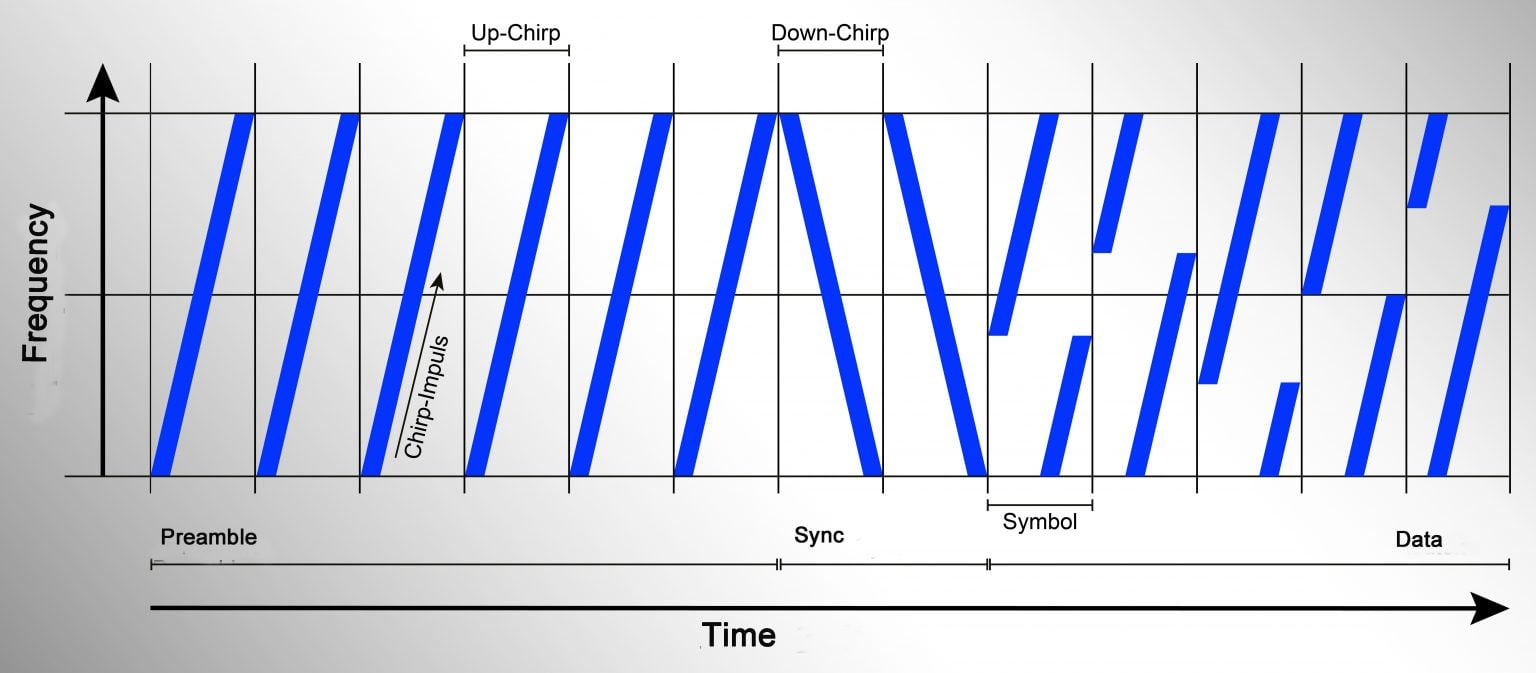
\includegraphics[width=0.7\linewidth]{./imagenes/css.jpg}
    \caption{Gráfico explicativo de modulación CSS~\cite{mokosmart_lora_frequency}. }
    \label{fig:css}
\end{figure}

LoRa se configura mediante la combinación de cuatro parámetros que permiten compensar el compromiso entre alcance, robustez, tasa de transferencia y consumo de energía. Estos son: 

\begin{itemize}
\item \textbf{Factor de dispersión (\textit{Spreading Factor}, SF)}. Puede variar entre SF7 y SF12. Representa el número de bits codificados por cada símbolo. Aumentar el SF duplica la duración de transmisión de un símbolo, mejorando la sensibilidad del receptor y el alcance a cambio de aumentar el Tiempo de permanencia en el aire (\textit{Time-on-Air}, ToA)~\cite{chaudhari2020lpwan}. 

\item \textbf{Ancho de banda (BW)}. Supone el rango de frecuencias asignados al canal. Normalmente se emplea 125~kHz, pudiendo ampliarse hasta 500~kHz. A mayor BW, mayor velocidad de transmisión, pero mayor es la potencia del ruido que se capta en la banda~\cite{devalal2018lora}.

\item \textbf{Tasa de codificación (\textit{Coding Rate}, CR)}. Determina la cantidad de bits de redundancia que se introducen para garantizar la corrección de posibles errores. Puede tomar los valores CR: 4/5, 4/6, 4/7 o 4/8~\cite{arregui2025gatewayfree}.

\item \textbf{Potencia de transmisión ($P_{TX}$)}. Configurable habitualmente entre 2 y 22~dBm según el transceptor, aunque el límite legal lo fija cada sub-banda de la normativa ETSI EN 300 220~\cite{etsien300F2202}. Determina el presupuesto de enlace (\textit{link budget}) del sistema, permitiendo alcanzar un margen de atenuación máximo (\textit{Maximum Allowable Path Loss}, MAPL) superior a los 150~dB~\cite{chaudhari2020lpwan}.
\end{itemize}

En general, la tecnología LoRa opera exclusivamente en la capa física (PHY) del modelo OSI, encargándose de la transmisión y recepción de tramas de radiofrecuencia mediante CSS, pero careciendo de mecanismos nativos para el control de acceso al medio (MAC), direccionamiento de dispositivos o gestión de la topología de red~\cite{arregui2025gatewayfree}. Por este motivo, para constituir una red de comunicaciones completa y funcional se requiere un protocolo de capa superior; en el estándar comercial dominante, esta función la desempeña el protocolo \textit{LoRaWAN}~\cite{devalal2018lora,sornin2015lorawan}.


\section{LoRaWAN y sus limitaciones en entornos locales}

El estándar LoRaWAN (\textit{Long Range Wide Area Network}), mantenido por la LoRa Alliance, define la pila de protocolos de capa superior (Control de Acceso al Medio y capa de red) que opera sobre la capa física LoRa. A diferencia de las redes locales punto a punto o en malla, la arquitectura de LoRaWAN se estructura bajo una topología en estrella de estrellas (\textit{star-of-stars})~\cite{loraalliance_home}. En ella, los nodos finales transmiten mediante enlaces LoRa de un solo salto a una o varios gateways, que reenvían las tramas por una red IP a un servidor de red. Este se encarga de eliminar duplicados, autenticar dispositivos y gestionar parámetros de la red, posteriormente un servidor de aplicación procesa los datos de usuario. En la figura~\ref{fig:lorawanARCH}, se muestra la arquitectura que posee LoRaWAN. 

\begin{figure}[htbp]
    \centering
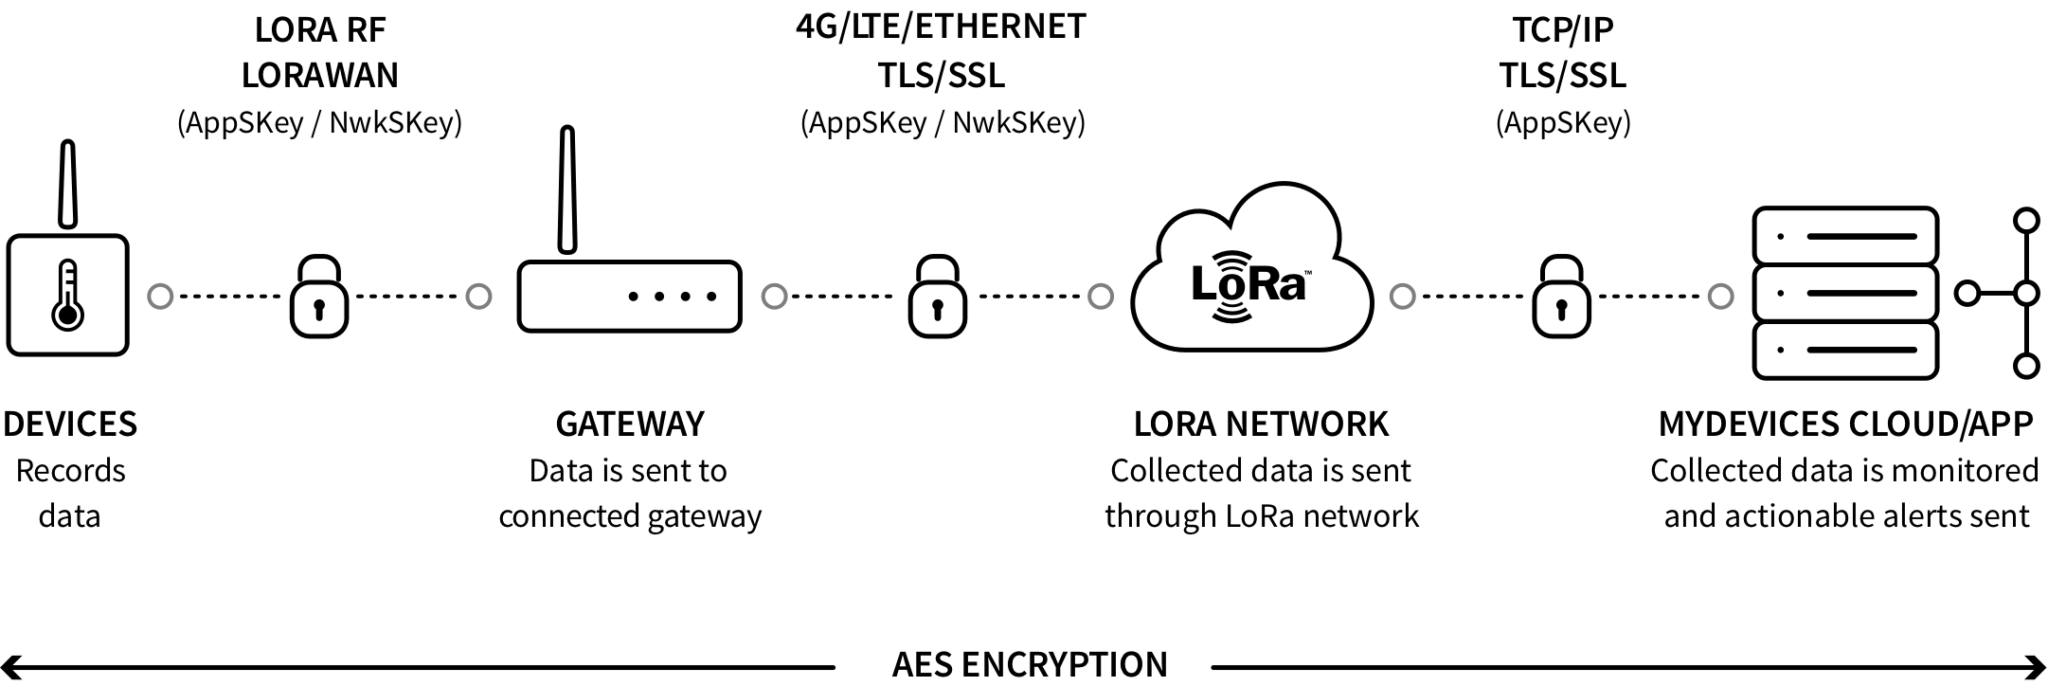
\includegraphics[width=1\linewidth]{./imagenes/lorawan.png}
    \caption{Arquitectura de LoRaWAN y sus distintos componentes~\cite{mydevices_lorawan}. }
    \label{fig:lorawanARCH}
\end{figure}

La especificación define tres clases de dispositivos finales. La clase A, obligatoria
y de menor consumo, abre dos ventanas de recepción tras cada transmisión
ascendente. La clase B añade ventanas de recepción programadas sincronizadas
mediante \textit{beacons}, y la clase C mantiene la recepción abierta de forma
casi continua, a costa de un mayor consumo.
El acceso al medio (MAC) es de tipo ALOHA puro, sin escucha previa del canal, y
queda sujeto a las restricciones de ciclo de trabajo (\textit{duty cycle}) de cada región. Para optimizar la capacidad, el servidor de red puede ajustar dinámicamente el SF y la potencia de los nodos mediante el mecanismo \textit{Adaptive Data Rate} (ADR). Respecto a la seguridad, se emplea AES-128 con dos claves de sesión: una de red, para garantizar la
integridad y autenticidad de los mensajes, y otra de aplicación, que cifra
la carga útil de extremo a extremo~\cite{sornin2015lorawan}.

Estas características convierten a LoRaWAN en una solución consolidada para
despliegues metropolitanos y rurales, pero resulta poco adecuada para una red local con requisitos de baja latencia. Su arquitectura depende de
pasarelas y de un servidor de red, a menudo operados por terceros, lo que añade un
coste de infraestructura~\cite{arregui2025gatewayfree}, y la comunicación descendente queda limitada a las ventanas de recepción de cada clase. Además,
el acceso ALOHA provoca más colisiones al aumentar la densidad de nodos,
lo que degrada la tasa de entrega de paquetes~\cite{adelantado2017limits}, la escalabilidad sigue siendo un reto~\cite{cotrim2020lorawan}.
Estas limitaciones motivan la aparición de alternativas.

\section{Protocolos alternativos y mecanismos de acceso al medio sobre LoRa}

La forma más sencilla de interconexión sobre la capa física LoRa consiste en la comunicación entre pares (\textit{peer-to-peer}, P2P). En este esquema, dos o más microcontroladores intercambian tramas de radiofrecuencia de forma directa sin necesidad de (\textit{gateways}) ni servidores de red en la nube, otorgando al desarrollador un control total sobre el formato de la trama, el control de acceso al medio y la seguridad de la red~\cite{alam2021smart}.

Sin embargo, para gestionar redes locales con múltiples dispositivos surge la necesidad de definir un mecanismo de acceso al medio eficiente. El protocolo estándar LoRaWAN utiliza por defecto un esquema ALOHA no ranurado, en el cual los nodos transmiten de manera asíncrona en el momento en que disponen de datos, sin verificar previamente si el canal radio está ocupado. ALOHA simplifica la arquitectura del nodo final pero sufre una degradación severa por colisiones de paquetes a medida que se incrementa la densidad de la red o la frecuencia del tráfico, impidiendo garantizar el determinismo temporal y la baja latencia que requieren ciertas aplicaciones, como la que se pretende desarrollar en este trabajo.

Para mitigar las limitaciones de ALOHA y evitar colisiones destructivas en el canal inalámbrico, la literatura académica ha explorado, entre otras, dos alternativas en la capa MAC:

\begin{enumerate}
    \item \textbf{Mecanismos basados en división temporal (TDMA / \textit{Slotted MAC})}: Dividen el tiempo de transmisión en ranuras discretas (\textit{time slots}) asignadas individualmente a cada nodo para erradicar las colisiones internas. Entre las propuestas pioneras destaca \textit{LoRaBlink}, basada en un protocolo de recolección en árbol con ranuras temporales~\cite{bor2016lora}, así como arquitecturas coordinadas que implementan sincronización en banda~\cite{farahani2026sdlora} para cumplir con plazos de entrega estrictos (\textit{deadlines}).
    \item \textbf{Mecanismos basados en escucha previa del canal (LBT / \textit{CSMA})}: Evalúan la presencia de portadora (\textit{Listen-Before-Talk}) antes de emitir y aplican temporizadores de espera aleatorios (\textit{backoff}) si el canal está ocupado. Proyectos de código abierto orientados a la mensajería sin infraestructura como \textit{Meshtastic}~\cite{meshtastic} utilizan este enfoque para coordinar nodos distribuidos de forma descentralizada.
\end{enumerate}

A partir de estos principios de acceso y coordinación se han desarrollado tanto mallas P2P sin pasarelas~\cite{berto2021lora} como soluciones multisalto sobre LoRaWAN~\cite{cotrim2020lorawan} y redes en malla (\textit{mesh}) multisalto generales~\cite{pueyo2021beyond}, en las que los nodos retransmiten paquetes de sus vecinos para extender la cobertura evitando la centralización en \textit{gateways}.

En este ámbito, Arregui Almeida \textit{et al.}~\cite{arregui2025gatewayfree} diseñan y validan una red en malla sin \textit{gateway} sobre microcontroladores de consumo ESP32-S3 con transceptores SX1262. Su propuesta integra encaminamiento por vecinos, confirmaciones salto a salto y acceso al canal de tipo \textit{Listen-Before-Talk} (LBT), obteniendo tasas de entrega de paquetes (PDR, \textit{Packet Delivery Ratio}) de hasta el 95\,\% en entornos controlados. Aunque la topología difiere de la arquitectura de área local en estrella prevista para el protocolo a desarrollar, este trabajo valida dos aspectos cruciales: la viabilidad técnica de implementar un protocolo sobre la capa física de LoRa personalizado sobre hardware de bajo coste (ESP32) y la eficacia de la escucha previa LBT como mecanismo de acceso al medio para reducir colisiones.

\section{Seguridad en redes LPWAN}

La seguridad en las redes LPWAN se basa en garantizar confidencialidad, integridad y autenticación de mensajes~\cite{iqbal2018aes}. La especificación de LoRaWAN, basa la seguridad en con doble capa basada en AES-128. La clave de sesión de red (NwkSKey) genera un código de integridad (MIC) de 32 bits sobre la trama, y la clave de sesión de aplicación (AppSKey) cifra la carga útil de extremo a extremo~\cite{sornin2015lorawan}.

Este método posee limitaciones prácticas. En muchos nodos comerciales el microcontrolador se comunica con el transceptor por UART o SPI sin cifrar. Un atacante con acceso al dispositivo puede capturar las claves de sesión y clonar el nodo. Además, el propio canal radio es abierto. Eso lo expone a interferencias deliberadas (\textit{jamming}), el cual es un problema muy presente en IoT~\cite{sigfox2017overview}. Por último, se pueden dar ataques de repetición cuando no se validan los contadores de trama~\cite{vodafone_nbiot}. Ambos ataques permiten, a su vez, ataques tipo \textit{wormhole}, en los que se suprimen mensajes legítimos y se reinyectan paquetes capturados anteriormente~\cite{chacko2018security}.


Tras revisar la literatura científica, se confirma la viabilidad de aplicar mecanismos de seguridad en dispositivos de bajo coste, Iqbal e Iqbal~\cite{iqbal2018aes} exponen un sistema de comunicación punto a punto seguro para microrredes usando AES sobre ESP32 con módulo LoRa, logrando autenticación mediante códigos de autenticación únicos por mensaje con enlaces de larga distancia y bajo consumo. Este resultado es directamente extrapolable a este trabajo, donde se emplea la misma combinación, ESP32 y transceptor LoRa.

\section{Microcontroladores para IoT: el ESP32}

El ESP32, desarrollado por Espressif Systems, se ha consolidado como plataforma de referencia para nodos IoT de bajo coste. Integra un procesador de doble núcleo Xtensa de hasta 240~MHz, memoria SRAM del orden de cientos de KB, buses SPI, UART e I$^2$C, aceleración criptográfica por hardware (AES, SHA y RSA) y conectividad Wi-Fi y Bluetooth~\cite{espressif_esp32_datasheet}. Esta capacidad de cómputo, muy superior a la de microcontroladores de 8 bits como el ATmega328, presentes en Arduino, permite ejecutar sobre el propio nodo una pila de red completa, incluyendo enrutamiento, gestión de tablas de vecinos y cifrado, sin depender de servidores externos.

En aplicaciones prácticas el ESP32 se combina con transceptores sub-GHz de Semtech como el SX1276 o el SX1262 comunicados a través de SPI~\cite{semtech_sx1262_datasheet}. Existen placas comerciales que integran ambos chips, la antena y una pantalla OLED, como las TTGO LoRa32 o la Heltec Wireless Stick V3. Esta última combina un ESP32-S3 con un SX1262 y es la plataforma utilizada por Arregui Almeida \textit{et al.}~\cite{arregui2025gatewayfree} para validar una red \textit{mesh} LoRa sin pasarelas.

\section{Síntesis del capítulo}

En conclusión, la revisión de la literatura muestra que la capa física LoRa permite desarrollar soluciones de comunicación de largo alcance y bajo coste. Aunque LoRaWAN proporciona una solución estandarizada y ampliamente utilizada, sus mecanismos de coordinación y su arquitectura no necesariamente se ajustan a las necesidades de todas las aplicaciones de IoT.


Por otra parte, los trabajos sobre redes P2P, arquitecturas en malla y mecanismos
alternativos de acceso al medio demuestran que es viable implementar protocolos
propios sobre LoRa con hardware de bajo coste como el ESP32. Ninguno de ellos,
sin embargo, reúne a la vez una infraestructura mínima y propia, un acceso al
medio coordinado y una respuesta inmediata en ambos sentidos. A partir de estos
antecedentes, este TFG propone LoRaLAN: un protocolo en estrella de un solo salto,
con una única pasarela gestionada por la propia institución, que no depende de
infraestructura de terceros e integra la seguridad en su diseño.

El objetivo es dar soporte a aplicaciones como la monitorización de aulas y el
registro presencial de la actividad docente en el Centro Universitario de Mérida.
Su viabilidad se evalúa experimentalmente en el Capítulo~\ref{chap:6},
en términos de tasa de entrega de paquetes, latencia y comportamiento ante
transmisiones concurrentes.

\chapter{Metodología y fase de análisis}\label{chap:3}

En este capítulo se describe, en primer lugar, la metodología de desarrollo utilizada y, posteriormente, se detalla el análisis previo al diseño, que comprende el escenario de uso, los requisitos que debe satisfacer el protocolo y la viabilidad técnica, económica y legal del trabajo.

Dado que este proyecto consiste en el diseño de un protocolo de comunicaciones, cuyo comportamiento depende de un canal de radio compartido y con pérdidas, no se ha seguido un modelo de desarrollo en cascada, en el que el diseño se cierra por completo antes de implementar y la validación se deja para el final. En un protocolo, buena parte de los problemas (colisiones, temporizadores mal dimensionados o interacciones inesperadas entre tramas) solo se manifiestan cuando el código se ejecuta, por lo que cualquier hallazgo durante la validación obliga a revisar el diseño.

Por este motivo, se ha seleccionado un modelo de desarrollo iterativo e incremental. No se ha aplicado de manera formal ninguna metodología ágil concreta, como podría ser Scrum, aunque sí se han adoptado sus principios básicos: incrementos pequeños y funcionales, y verificación continua.

\section{Metodología de desarrollo}\label{sec:metodologia}

El modelo iterativo e incremental divide el desarrollo en ciclos cortos, cada uno de los cuales añade una funcionalidad concreta sobre una versión del sistema que ya funciona. En este trabajo, cada iteración se compone de cuatro actividades: análisis, diseño, implementación y verificación. En el análisis se identifican la funcionalidad que se va a incorporar y los requisitos a los que responde. En el diseño se definen los elementos que forman parte del protocolo: formato de paquete, mecanismos de sincronización, políticas de reintentos, etc. En la implementación se codifica el incremento en la librería. Por último, en la verificación se comprueba el incremento y se revisa que no haya alterado el comportamiento de lo ya construido.

\section{Análisis del sistema en el que se basa el protocolo}\label{sec:escenario}

Como se ha comentado, el objetivo de este trabajo es desarrollar un protocolo de comunicación de área local sobre la capa física de LoRa para una aplicación concreta.

El sistema a desarrollar es una aplicación de registro de clases y monitoreo de aulas. Con esta herramienta, se pretende proporcionar a los profesores un sistema que permita registrar sus clases empleando una tarjeta NFC de forma más sencilla. Actualmente, se emplea un portal web al que los docentes deben acceder mediante certificado digital para registrar las clases. Por otro lado, se pretende recoger información sobre las aulas, como la humedad, la temperatura, la luminosidad y detección de presencia. Con esto se proporciona a los conserjes una herramienta que les permita monitorear las aulas de un vistazo con la capacidad de gestionar remotamente el sistema de climatización y las persianas. 

El escenario de referencia es un edificio, concretamente el aulario del centro universitario, con una veintena de aulas repartidas en dos plantas. Las distancias entre cualquier aula y un punto central del edificio son de decenas de metros, con muros intermedios. Los dispositivos están alimentados desde la red eléctrica, por lo que el consumo no es, en principio, una restricción relevante.

En este escenario intervienen los siguientes elementos:

\begin{itemize}
\item \textbf{Nodo de aula}: Dispositivo instalado en cada aula, con lector NFC, sensores ambientales y relés.
\item \textbf{Gateway}: Dispositivo único del sistema que gestiona la red de nodos, con conexión hacia el servidor y capacidad de alojar en local el propio servidor y la base de datos.
\item \textbf{Servidor web}: Aloja la lógica de la aplicación y la base de datos, y queda fuera de la red de radio.
\item \textbf{Usuarios}: Habrá tres tipos de usuarios del sistema: profesores, conserjes y administradores.
\end{itemize}

El escenario genera tres clases de tráfico con exigencias muy distintas, que son las que determinan el diseño del acceso al medio. En la Tabla~\ref{tab:trafico} se muestran dichas clases.

\begin{table}[htbp]
\centering
\caption{Clases de tráfico del escenario de uso.}\label{tab:trafico}
\renewcommand{\arraystretch}{1.3}
\begin{tabularx}{\textwidth}{p{2.4cm} p{2.4cm} p{2.4cm} X}
\toprule
\textbf{Tráfico} & \textbf{Sentido} & \textbf{Patrón} & \textbf{Exigencia} \\
\midrule
Evento (fichaje) & Nodo $\rightarrow$ gateway, con respuesta & Esporádico e imprevisible & Respuesta al usuario del orden de un segundo. No puede perderse, falsificarse ni duplicarse. \\
\midrule
Telemetría (sensores, estado) & Nodo $\rightarrow$ gateway & Periódico & Tolera retardos de decenas de segundos y la pérdida ocasional de una muestra. \\
\midrule
Órdenes (relés, reinicio) & Gateway $\rightarrow$ nodo & Esporádico & Efecto en pocos segundos. Debe confirmarse. \\
\bottomrule
\end{tabularx}
\end{table}

Como se observa en la Tabla~\ref{tab:trafico}, el tráfico periódico es predecible y admite planificación, mientras que el evento es urgente pero infrecuente y la orden exige que el nodo sea alcanzable en cualquier momento. Por tanto, ningún esquema de acceso único sirve adecuadamente a las tres clases.

\subsection{Requisitos del sistema}

Los requisitos funcionales del sistema se agrupan en cinco bloques.

El primero es el fichaje. El profesor ficha acercando su tarjeta NFC al nodo del aula \textbf{(SIS-1)}. El servidor valida el fichaje comprobando que la tarjeta esté registrada, que el nodo tenga un aula asignada, que haya una clase en curso y que esa clase sea de ese profesor \textbf{(SIS-2)}. El nodo recibe el resultado, que puede ser OK, sin clase, denegado, desconocido o reintentar \textbf{(SIS-3)}, y el sistema garantiza que ningún fichaje se pierda ni se registre dos veces \textbf{(SIS-4)}.

El segundo bloque es la monitorización del aula. El nodo mide temperatura, humedad, presión, luz y presencia, y envía los datos periódicamente \textbf{(SIS-5)}. El conserje y el administrador pueden ver el estado de cada aula y si su nodo está en línea \textbf{(SIS-6)}.

El tercero es el control remoto. El conserje y el administrador pueden encender y apagar la calefacción y la iluminación de un aula \textbf{(SIS-7)}. Además, el administrador puede reiniciar los nodos y asignarles un aula \textbf{(SIS-8)}.

El cuarto es la gestión de datos y usuarios. El administrador gestiona usuarios, aulas, clases y asistencias \textbf{(SIS-9)}, y el profesor consulta su historial de asistencias \textbf{(SIS-10)}. Los usuarios inician sesión con correo y contraseña, y cada rol accede a su propio panel \textbf{(SIS-11)}.

Por último, el sistema obtiene el horario de clases de la base de datos y, si no está disponible allí, lo solicita al servicio de reservas de la universidad \textbf{(SIS-12)}.

\section{Especificación de requisitos del protocolo LoRaLAN}\label{sec:requisitos}

Tras la recogida de requisitos del sistema de registro de clases y monitoreo de aulas, se procede a la elaboración de la especificación de requisitos del protocolo a desarrollar. 

\subsection{Requisitos funcionales}

\begin{longtable}{@{}l p{0.26\textwidth} p{0.52\textwidth}@{}}
\caption{Requisitos funcionales del protocolo LoRaLAN.}\label{tab:pro}\\
\toprule
\textbf{ID} & \textbf{Requisito} & \textbf{Descripción} \\
\midrule
\endfirsthead
\toprule
\textbf{ID} & \textbf{Requisito} & \textbf{Descripción} \\
\midrule
\endhead
\bottomrule
\endfoot
PRO-1 & Comunicación entre nodos y gateway & El protocolo debe permitir la comunicación entre un gateway y múltiples nodos pertenecientes a una misma red. \\
\midrule
PRO-2 & Transmisión de telemetría & El protocolo debe permitir que los nodos transmitan datos de telemetría al gateway de forma periódica y que el gateway detecte los nodos inactivos. \\
\midrule
PRO-3 & Comunicación de eventos asíncronos & El protocolo debe permitir que los nodos comuniquen eventos al gateway sin depender exclusivamente de la comunicación periódica, comprobando previamente que el canal esté libre, y que reciban en la confirmación un código de estado de la aplicación. \\
\midrule
PRO-4 & Comunicación descendente & El protocolo debe permitir que el gateway envíe órdenes y mensajes dirigidos a nodos concretos, de modo que una orden se ejecute como mucho una vez. \\
\midrule
PRO-5 & Confirmación de entrega & El protocolo debe confirmar la recepción de los mensajes que lo requieran, de modo que la confirmación garantice la entrega. Ante la falta de confirmación, debe retransmitir un número acotado de veces, informar a la aplicación si no logra la entrega y permitir que un evento se entregue por la vía del sondeo. \\
\midrule
PRO-6 & Gestión de la incorporación y salida de nodos & El protocolo debe permitir la incorporación autenticada de nodos a la red y su posterior salida de forma controlada. \\
\midrule
PRO-7 & Sincronización temporal & El protocolo debe permitir distribuir referencias temporales desde el gateway a los nodos. \\
\midrule
PRO-8 & Seguridad de las comunicaciones & El protocolo debe proporcionar mecanismos que garanticen la confidencialidad, autenticidad e integridad de los mensajes, además de protección frente a repetición. \\
\midrule
PRO-9 & Recuperación ante la pérdida del gateway & Un nodo asociado debe detectar la ausencia prolongada de tráfico dirigido a él y volver a asociarse sin reiniciarse. El plazo de detección debe ser configurable y superior al tiempo entre dos turnos de sondeo del nodo. \\
\end{longtable}

\subsection{Requisitos no funcionales}
\begin{table}[htbp]
    \centering
    \caption{Requisitos no funcionales del protocolo.}
    \label{tab:requisitos-no-funcionales}
    \renewcommand{\arraystretch}{1.3}
    \begin{tabularx}{\textwidth}{l l X}
        \toprule
        \textbf{ID} & \textbf{Requisito} & \textbf{Descripción} \\
        \midrule
        RNF-1 & Eficiencia & El protocolo debe minimizar la latencia de las comunicaciones y el tiempo de ocupación del canal radio. \\\midrule
        RNF-2 & Cumplimiento normativo & El funcionamiento debe respetar las restricciones de uso radioeléctrico aplicables a la sub-banda seleccionada~\cite{etsien3002202,ercrec7003}. \\ \midrule
        RNF-3 & Recursos y capacidad & La implementación debe funcionar sobre hardware de bajo coste, utilizar memoria estática y admitir al menos 32 nodos mediante estructuras de tamaño fijo. La carga útil de las tramas no debe superar los 64~bytes. \\ \midrule
        RNF-4 & Portabilidad e integración & El protocolo debe implementarse como una librería independiente de la aplicación y adaptable a distintos transceptores compatibles, con una interfaz sencilla de utilizar. \\ \midrule
        RNF-5 & Verificabilidad & La lógica del protocolo debe poder probarse de forma determinista y repetible sin necesidad de hardware físico. \\ 
        \bottomrule
    \end{tabularx}
\end{table}

\section{Caracterización del espectro con radio definida por software}\label{sec:sdr}

Antes de diseñar y desarrollar el protocolo se debe confirmar que el canal de radio en la localización donde se desplegaría no está excesivamente ocupado, ya que un canal con mucho tráfico degradaría la calidad de la conexión provocando colisiones. 


Por tanto, se midió la ocupación real de la banda en la que puede operar LoRa en el aulario, empleando para ello una radio definida por software HackRF One~\cite{hackrfone}. El objetivo es, por un lado, determinar la actividad existente, ya que en el centro opera un gateway LoRaWAN, y, por otro lado, localizar la sub-banda disponible que más conviene para este sistema. A continuación, se introduce la banda en la que opera LoRa en Europa.

\subsection{Bandas ISM y de dispositivos de corto alcance}
\label{subsec:banda-ism}

Las bandas ISM son fragmentos del espectro radioeléctrico que la Unión Internacional de Telecomunicaciones (UIT) reservó para aplicaciones industriales, científicas y médicas. Se han consolidado como el espacio habitual para comunicaciones de uso libre porque no requieren licencia. Para operar en ellas, los equipos deben cumplir unas condiciones técnicas comunes y aceptar las interferencias sin derecho a protección~\cite{uitrr}.

En Europa, LoRa opera en la banda de 863--870~MHz (EU868). Aunque suele llamarse ISM, en sentido estricto es una banda para dispositivos de corto alcance (SRD, \textit{Short Range Devices}). Su uso está definido en la Unión Europea por la Decisión 2006/771/CE y sus modificaciones~\cite{decision2006771,decision20191345}, de obligado cumplimiento para los Estados miembros, que en España se aplica a través del Cuadro Nacional de Atribución de Frecuencias (CNAF)~\cite{cnaf2026}. Los equipos deben cumplir además la norma técnica ETSI EN~300~220~\cite{etsien3002202}. La banda se divide en sub-bandas con límites de potencia radiada aparente (PRA)\footnote{Potencia que un transmisor entrega a la antena multiplicada por la ganancia de dicha antena, en una dirección determinada, tomando como referencia un dipolo de media onda~\cite{raing_pra}.} y de ciclo de trabajo (\textit{duty cycle}), es decir, la fracción máxima de tiempo por hora que un dispositivo puede transmitir. Como alternativa al ciclo de trabajo, se pueden usar mecanismos de escucha previa y agilidad de frecuencia (LBT+AFA, \textit{Listen Before Talk} y \textit{Adaptive Frequency Agility}) como requisitos para operar en estas bandas. La Tabla~\ref{tab:subbandas-868} resume las principales sub-bandas~\cite{ercrec7003}.
\begin{table}[htbp]
    \centering
    \caption{Principales sub-bandas de la banda de 868~MHz para dispositivos de corto alcance de uso genérico~\cite{ercrec7003}.}
    \label{tab:subbandas-868}
    \renewcommand{\arraystretch}{1.3}
    \begin{tabular}{l c c}
        \toprule
        \textbf{Rango de frecuencias} & \textbf{PRA máxima} & \textbf{Ciclo de trabajo} \\
        \midrule
        863,0--865,0~MHz & 25~mW & 0,1\,\% \\
        865,0--868,0~MHz & 25~mW & 1\,\% \\
        868,0--868,6~MHz & 25~mW & 1\,\% \\
        868,7--869,2~MHz & 25~mW & 0,1\,\% \\
        869,4--869,65~MHz & 500~mW & 10\,\% \\
        869,7--870,0~MHz & 5~mW / 25~mW & Sin límite / 1\,\% \\
        \bottomrule
    \end{tabular}
\end{table}

Inicialmente, lo ideal sería desplegar el sistema sobre la sub-banda de 869,4--869,65~MHz, ya que es la menos restrictiva, aunque no puede afirmarse que sea la mejor opción sin medir el uso del canal.

\subsection{El procedimiento empleado para la medición}

Se definió un único punto de medida, situado en el aulario, que es el escenario objetivo. Se realizó una captura larga, de una hora ininterrumpida, puesto que esta duración es necesaria para estimar la ocupación de transmisores esporádicos.

Para la medición se empleó la herramienta \texttt{hackrf\_sweep}, que barre repetidamente el rango indicado y vuelca a un fichero de texto la potencia medida en cada intervalo de frecuencia. La resolución fue de 98~kHz por intervalo, del orden del ancho de un canal LoRa de 125~kHz. La captura larga del aulario se realizó el 5 de febrero de 2026, entre las 11:41 y las 12:41, y contiene un total de 1\,464\,485 barridos de la banda.

\begin{figure}[htbp]
    \centering
    \begin{subfigure}[b]{0.48\textwidth}
        \centering
        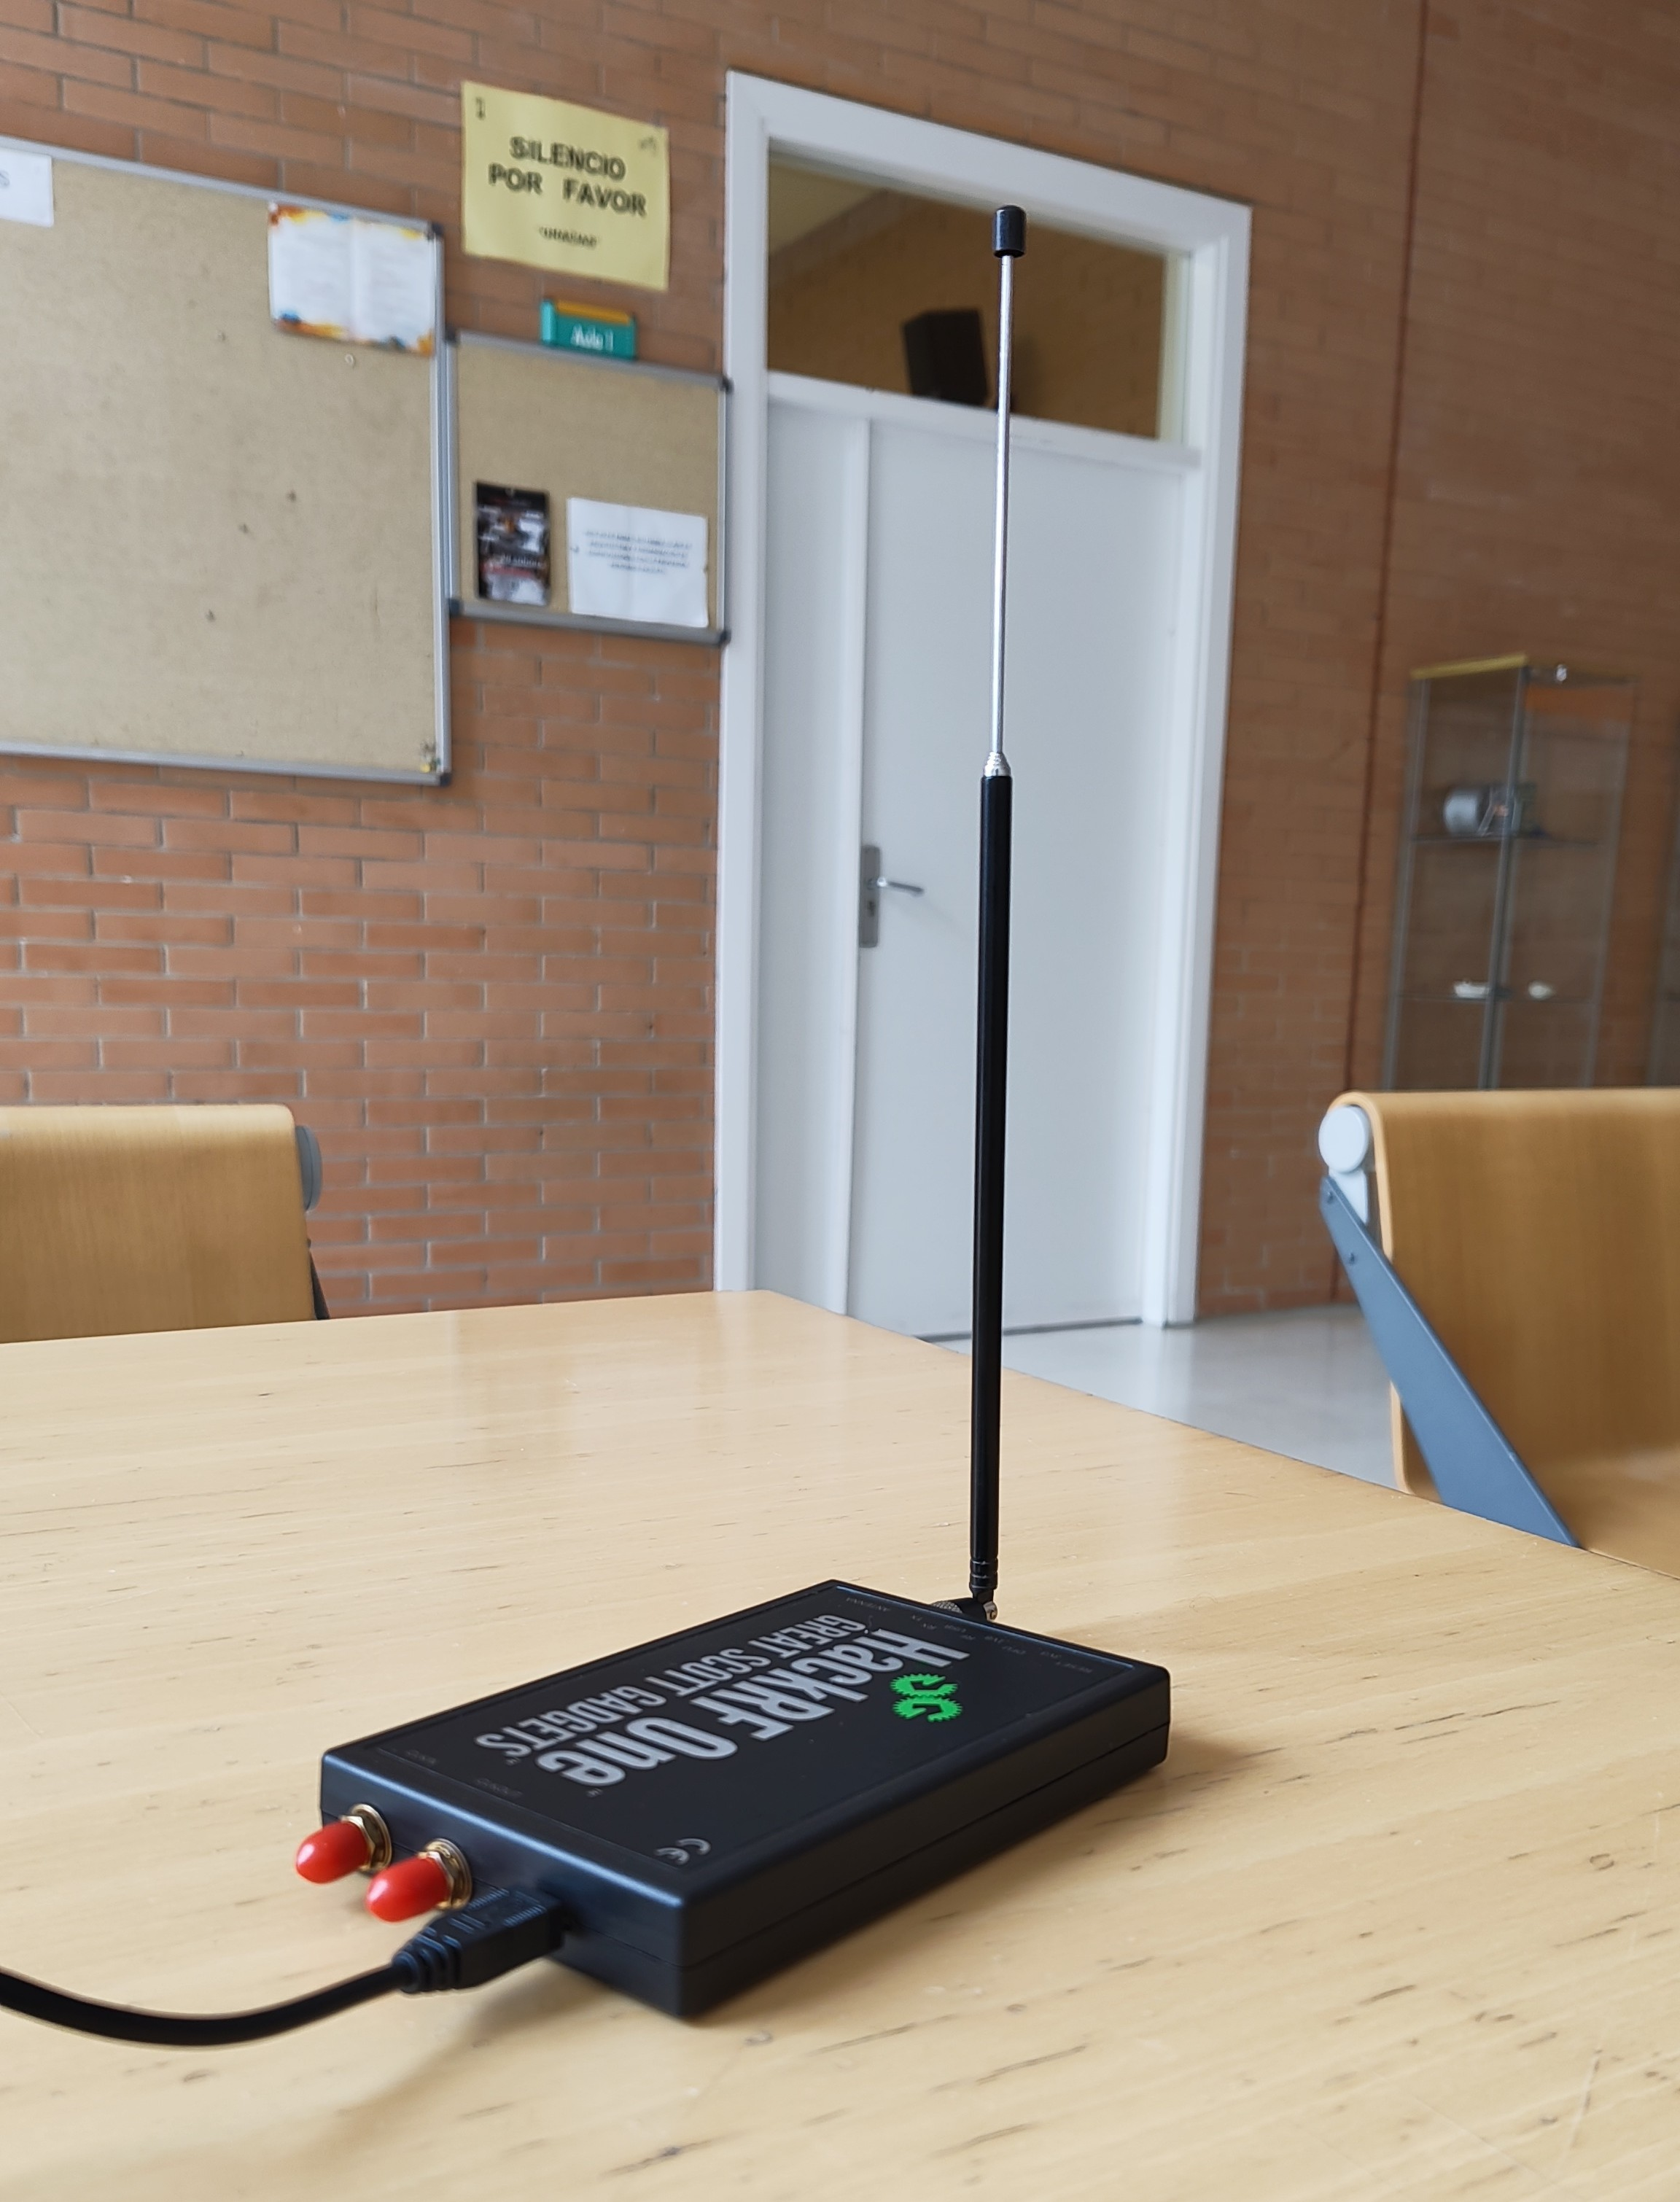
\includegraphics[width=\textwidth]{imagenes/sdr.jpg}
        \caption{Montaje empleado para la medición}
        \label{fig:sdr}
    \end{subfigure}
    \hfill
    \begin{subfigure}[b]{0.48\textwidth}
        \centering
        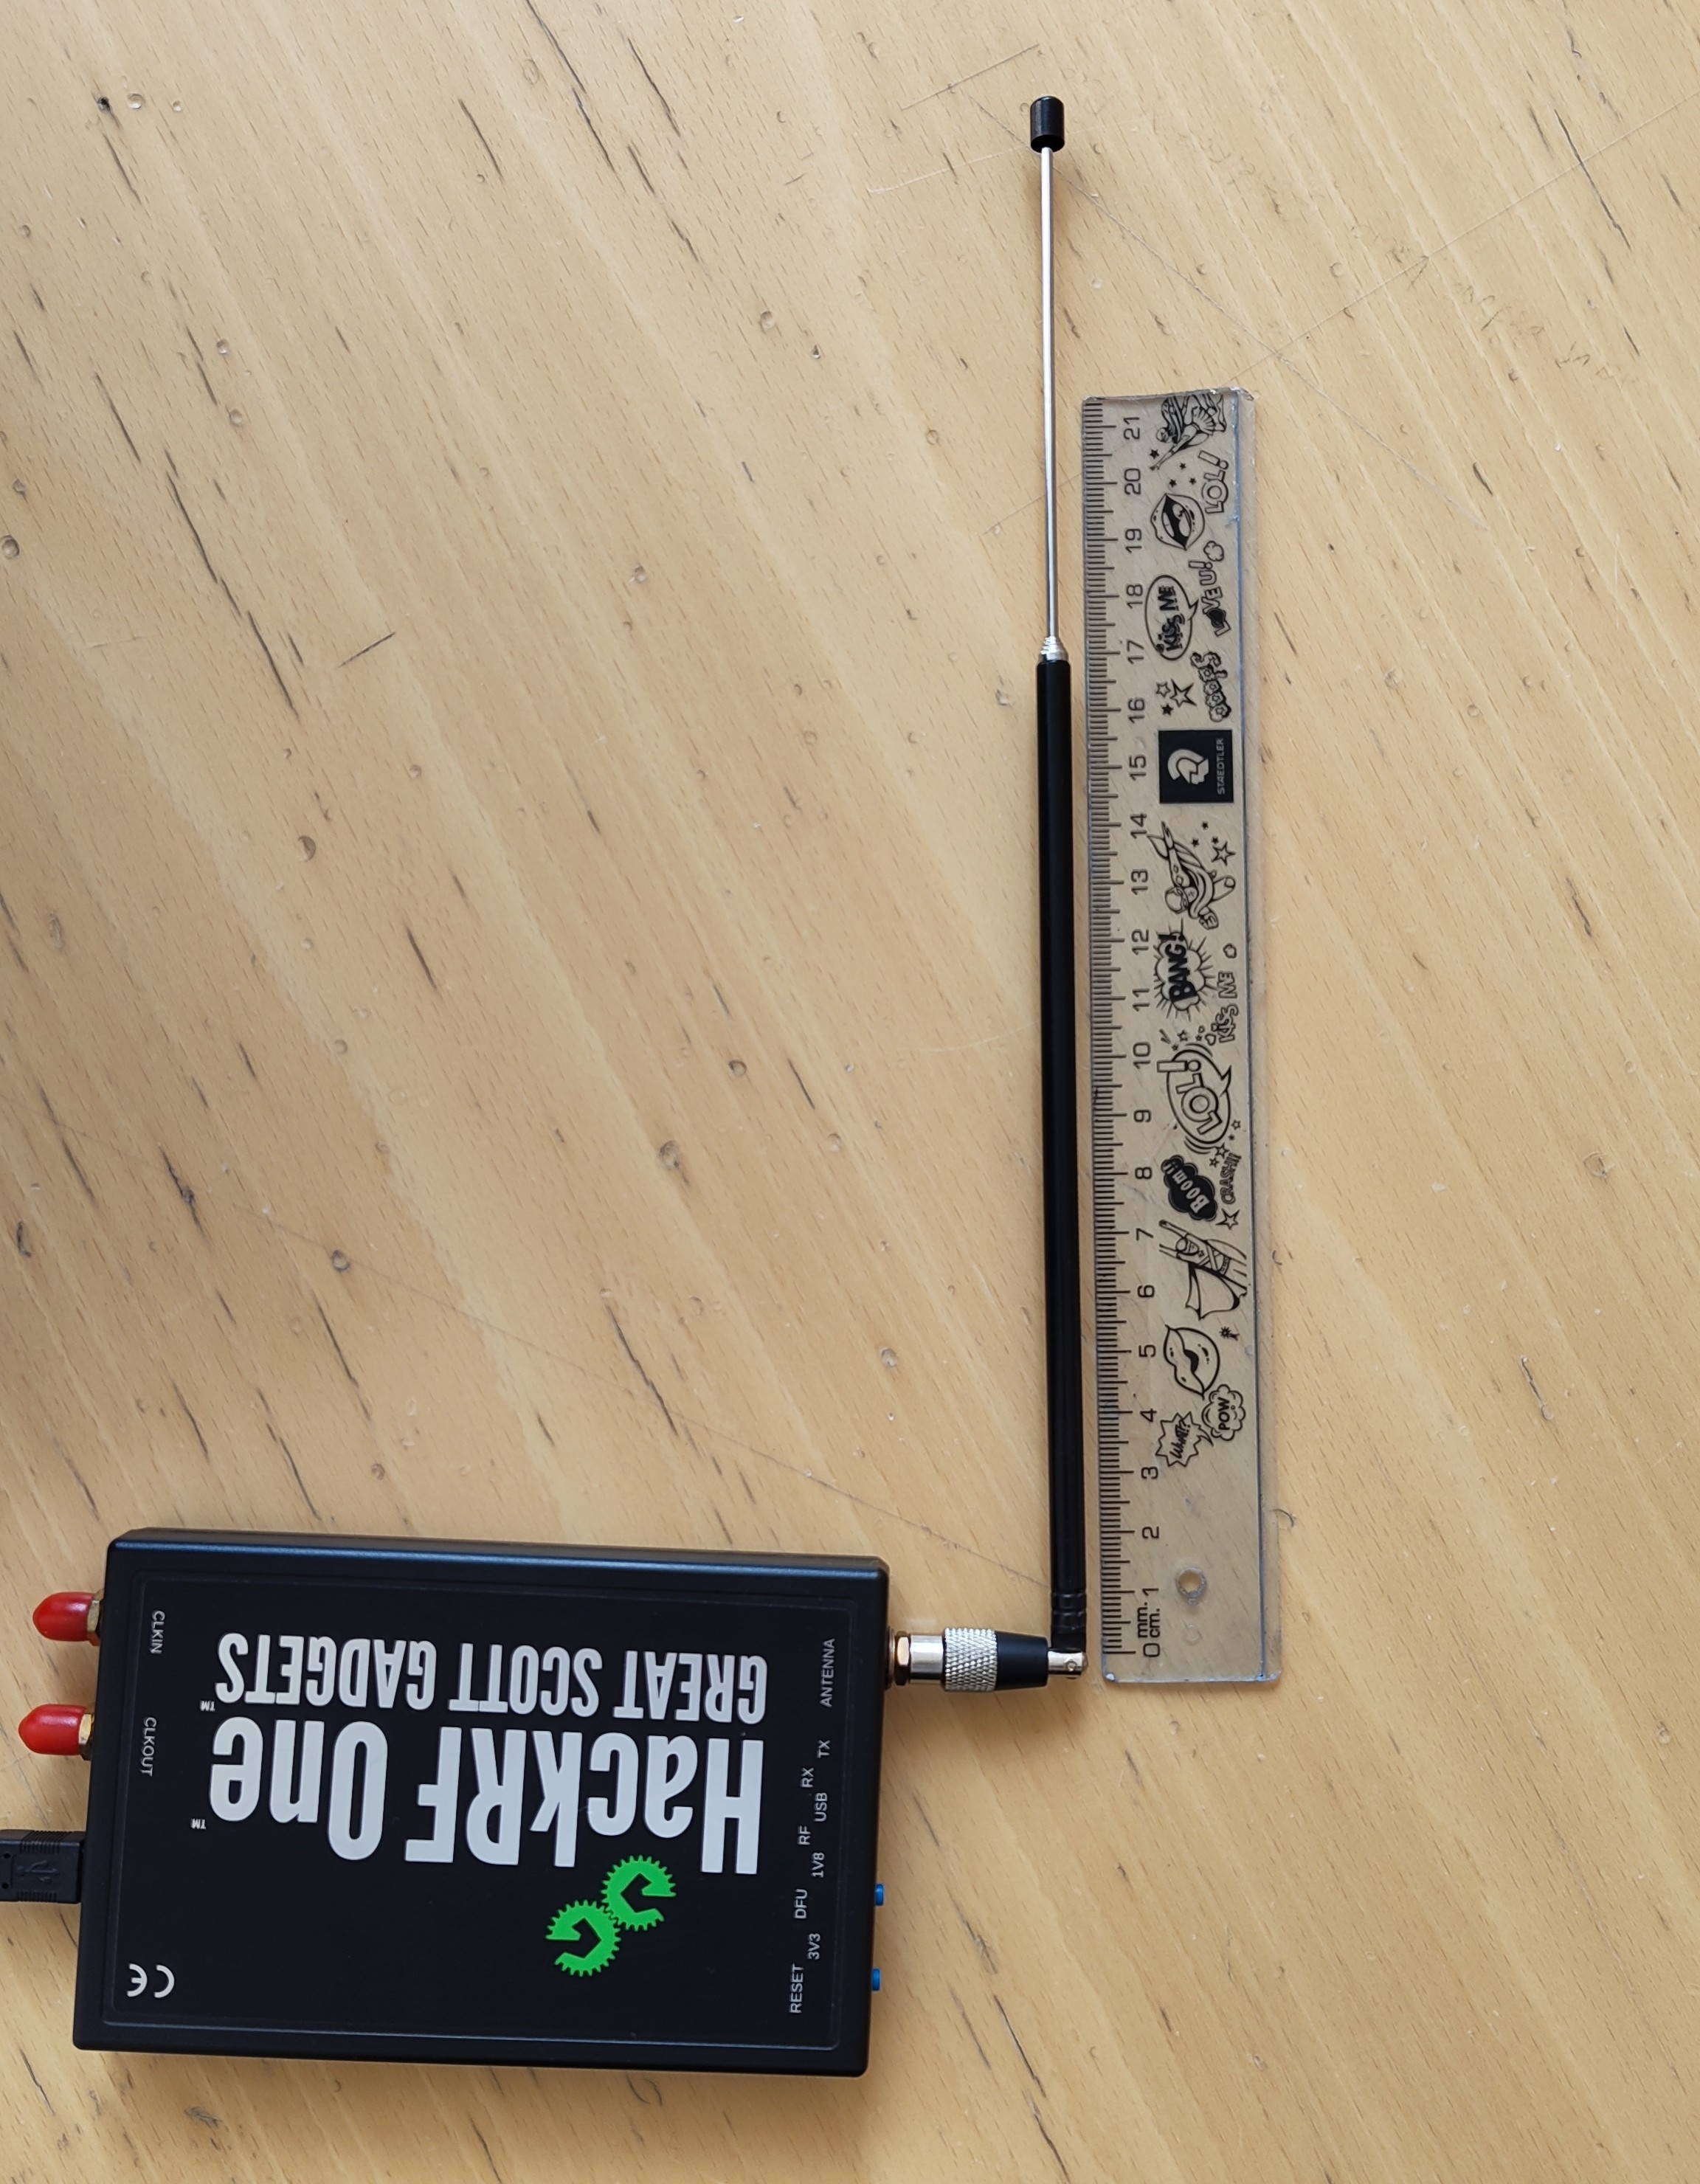
\includegraphics[width=\textwidth]{imagenes/sdr2.jpg}
        \caption{Medición de la antena telescópica}
        \label{fig:sdr2}
    \end{subfigure}
    \caption{Medición del espectro con HackRF One en el aulario.}
    \label{fig:conjunto}
\end{figure}

En la Figura~\ref{fig:sdr} se muestra el montaje realizado. Aunque no se puede apreciar en la imagen, la antena telescópica mide 26~cm. Esta antena funciona como un monopolo, que resuena cuando su longitud es un múltiplo impar de un cuarto de la longitud de onda ($\lambda/4$). A la frecuencia de trabajo, de aproximadamente 868~MHz, la longitud de onda es:

\begin{equation}
    \lambda = \frac{c}{f} = \frac{3 \cdot 10^{8}~\text{m/s}}{868 \cdot 10^{6}~\text{Hz}} \approx 34{,}6~\text{cm}
\end{equation}

Por ello, la antena se ajustó a una longitud de $3\lambda/4 \approx 26$~cm. Con esta longitud se mejora la adaptación de impedancias con el receptor y se reducen las pérdidas por reflexión.


El procesado se realizó mediante un \textit{script} en Python (Pandas, NumPy y Matplotlib), calculando sobre los datos obtenidos las tres métricas siguientes:

\begin{itemize}
\item \textbf{Potencia de ruido}: Potencia media de cada intervalo en ausencia de transmisiones.

\item \textbf{Valor máximo (\textit{max hold})}: Mayor potencia registrada en cada intervalo durante toda la captura. Revela transmisores potentes o cercanos, aunque emitan durante poco tiempo.

\item \textbf{Ocupación}: Porcentaje de barridos en los que la potencia de un intervalo supera un umbral situado por encima del ruido, fijado en $-55$~dBFS (unos 12~dB sobre el piso).
\end{itemize}

Las potencias se expresan en dBFS, es decir, son relativas al fondo de escala del conversor de la radio. Como el HackRF no está calibrado en potencia absoluta, las cifras son válidas para comparar frecuencias entre sí, pero no como medidas en dBm.

\subsection{Resultados y conclusiones de las mediciones}

En la Figura~\ref{fig:espectro} se resume la captura de una hora realizada en el aulario.
\begin{figure}[htbp]
\centering
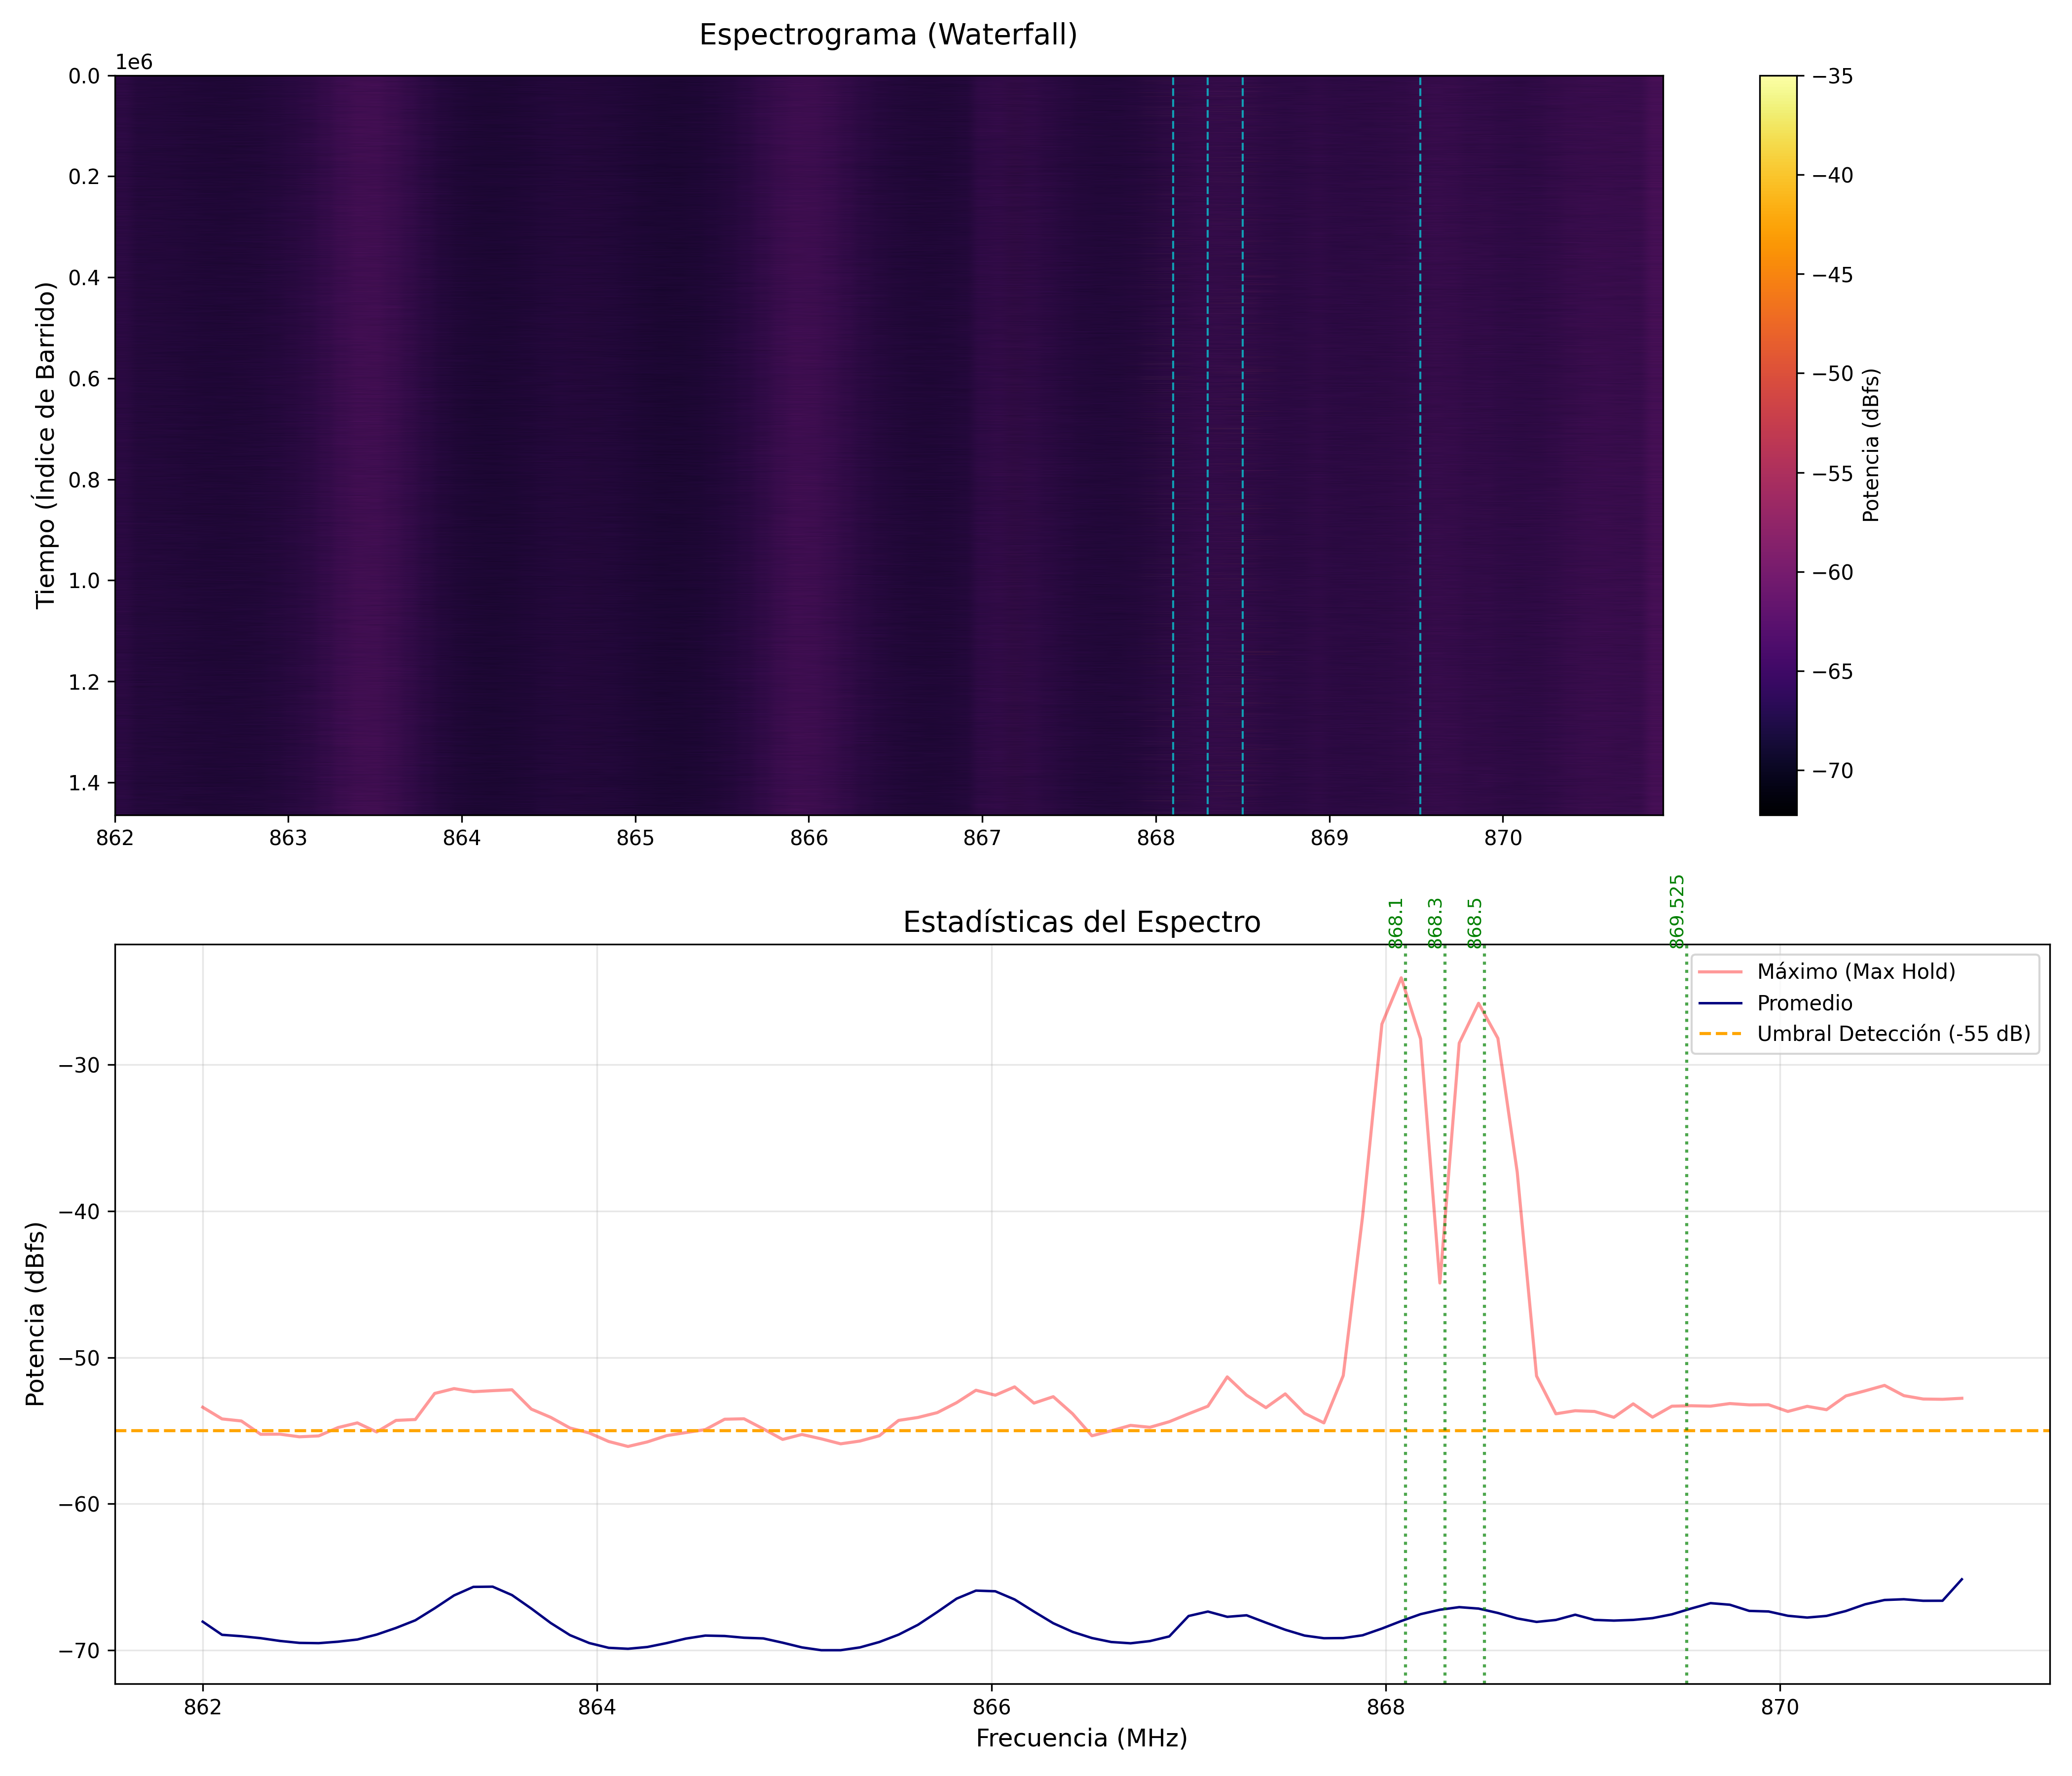
\includegraphics[width=\textwidth]{imagenes/analisis_lora_vertical_prueba.png}
\caption{\label{fig:espectro} Captura de una hora en el aulario (863--870~MHz). Arriba: espectrograma. Abajo: valor máximo y valor medio por frecuencia.}
\end{figure}

\begin{figure}[htbp]
\centering
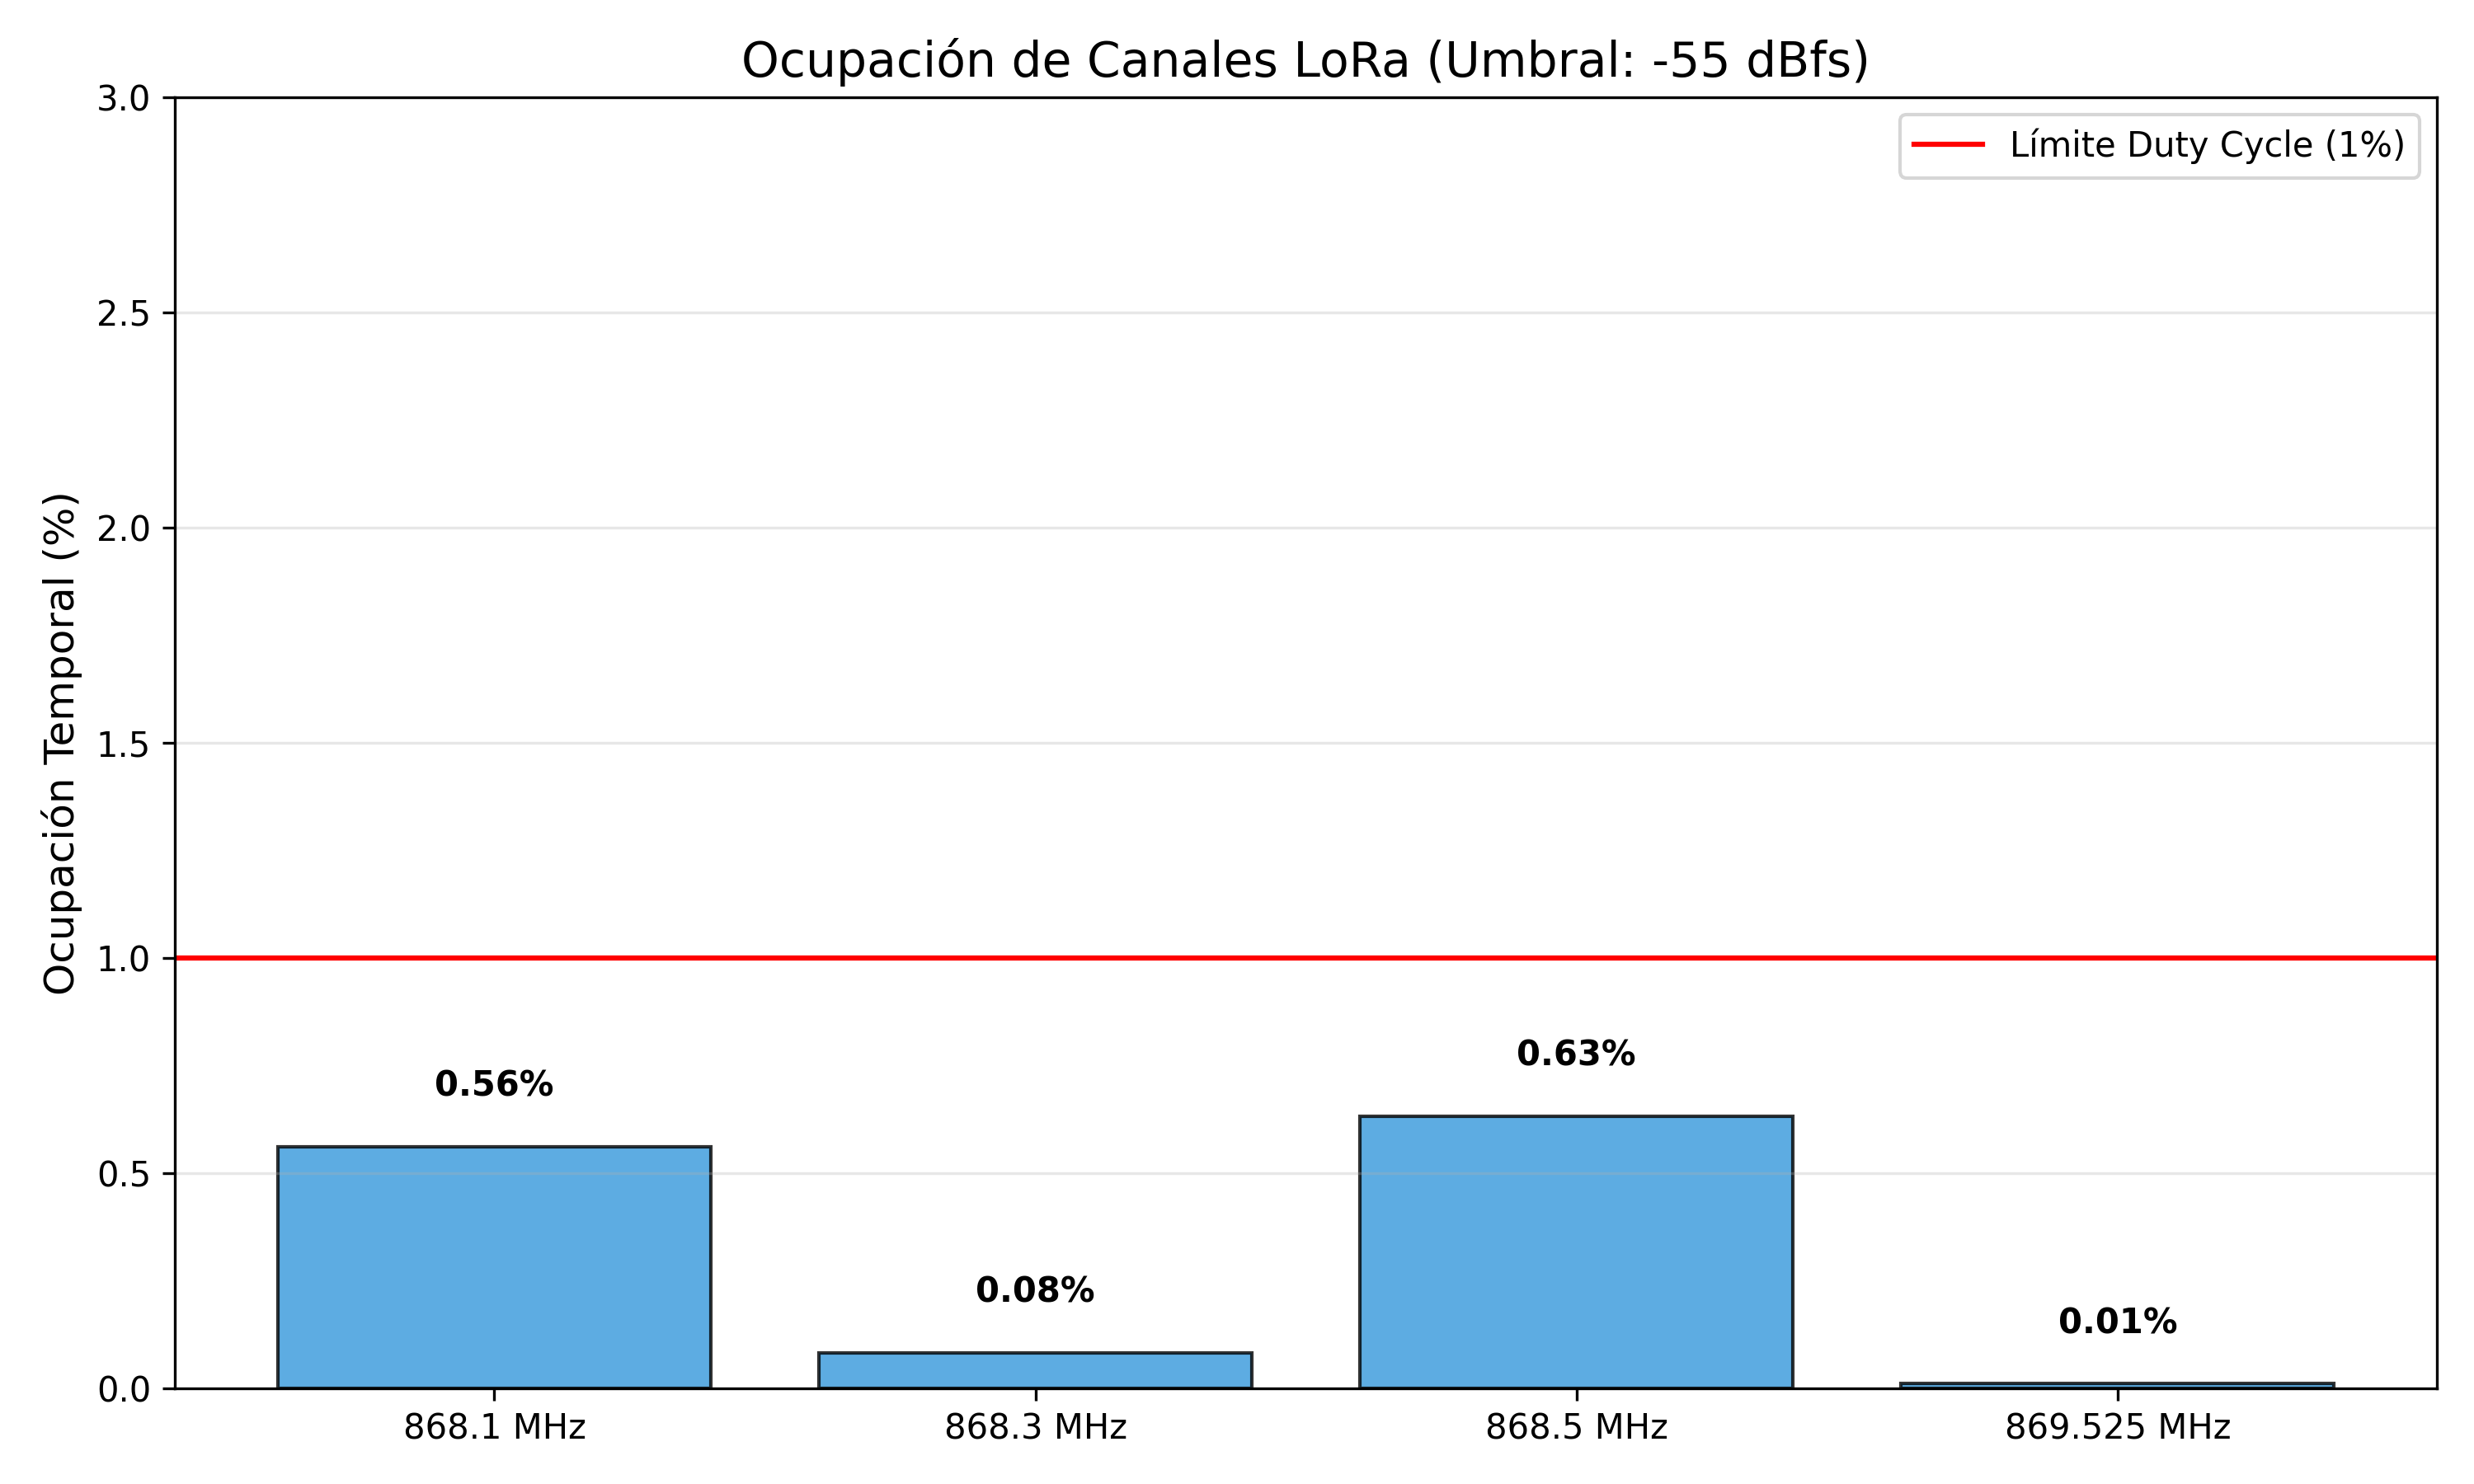
\includegraphics[width=\textwidth]{imagenes/histograma_ocupacion_lora_prueba.png}
\caption{\label{fig:DC} Gráfica de ocupación media de las distintas bandas disponibles.}
\end{figure}

Como se observa en la Figura~\ref{fig:espectro}, el piso de ruido es uniforme en toda la banda, en torno a $-67$~dBFS. La única actividad claramente distinguible del ruido se concentra entre 868,0 y 868,6~MHz, zona en la que se sitúan los canales ascendentes obligatorios de LoRaWAN. Sus picos superan el piso de ruido en más de 40~dB, lo que indica la presencia de transmisores cercanos, y la ocupación medida es de alrededor del 0,5\,\% por canal, como se puede observar en la Figura~\ref{fig:DC}.

En el resto de la banda el valor máximo no se separa del ruido: no se registró ninguna emisión apreciable durante la hora de captura. En particular, en la sub-banda de 869,4--869,65~MHz la ocupación es dos órdenes de magnitud inferior a la de los canales LoRaWAN y corresponde a picos de ruido.

Ante estos resultados, se selecciona como canal de operación la frecuencia de \textbf{869,525~MHz}, situada en la sub-banda de 869,4--869,65~MHz. Esta elección se debe a que ofrece un ciclo de trabajo mayor (máx. 10\,\%, frente al 1\,\% de la sub-banda de 868,0--868,6~MHz) y a que evita los canales que utiliza el tráfico LoRaWAN.

No obstante, esta elección conlleva un riesgo. La frecuencia seleccionada es también la que LoRaWAN emplea por defecto en su segunda ventana de recepción descendente, con SF12, por lo que, si el gateway LoRaWAN cercano la utilizase, interferiría con la red, aunque la captura no registró emisiones en ella.

\section{Viabilidad del proyecto}\label{sec:viabilidad}

Desde el punto de vista técnico, el proyecto es viable gracias a la disponibilidad de transceptores LoRa, hardware de bajo coste (microcontroladores y sensores) y herramientas de desarrollo software. El escenario de implementación, con unas veinte aulas y distancias reducidas, permite abordar el desarrollo sin requisitos exigentes de cobertura o consumo energético. Aun así, el funcionamiento deberá validarse mediante las pruebas previstas durante la implementación.

En cuanto a la viabilidad legal, la frecuencia seleccionada, 869,525~MHz, pertenece a una sub-banda que permite un ciclo de trabajo de hasta el 10\,\%. Su utilización queda condicionada al cumplimiento de los límites de potencia y del resto de requisitos radioeléctricos aplicables.

Por último, la viabilidad económica se apoya en el uso de componentes de bajo coste y herramientas de software libre, así como en la posibilidad de alojar el servidor y la base de datos en el gateway que se ejecutará sobre una Raspberry Pi. El coste definitivo del despliegue dependerá de los componentes seleccionados y de las necesidades de instalación del conjunto de nodos. En el Anexo~\ref{anexo_B} se recoge el presupuesto estimado para implementar un nodo y el gateway.
\chapter{Diseño del protocolo LoRaLAN}\label{chap:4}

En este capítulo se especifica el protocolo LoRaLAN. En primer lugar, se presentan su topología y los principios que han guiado su diseño. Posteriormente, se detallan todas las decisiones de diseño tomadas sobre el protocolo. Los repositorios que contienen el código están todos en el Anexo \ref{anexo:repos}.


\section{Visión general}

\textbf{LoRaLAN} es un protocolo de comunicación para redes de área local construido directamente sobre la capa física LoRa \cite{semtech_sx1276}. Define los mecanismos de las capas de enlace y de red necesarios para gestionar una red de un solo salto, incluyendo la delimitación y el direccionamiento de tramas, el acceso al medio, la fiabilidad de las comunicaciones, la asociación de dispositivos y la seguridad.

La red adopta una topología en \textbf{estrella}, con un único gateway y hasta 32 nodos en esta versión. Todos los nodos tienen al gateway en el otro extremo, por lo que los nodos no se comunican entre sí. Los dos roles que intervienen son los siguientes:

\begin{itemize}
\item \textbf{Nodo}: Es el dispositivo final. Gestiona la lógica de negocio de la aplicación correspondiente, se asocia al gateway, le envía eventos y telemetría y responde a sondeos e instrucciones cuando el gateway se lo solicita.

\item \textbf{Gateway}: Se encarga de coordinar la red. Permite la unión de nodos a la red, los sondea por turnos, difunde la hora, recibe sus eventos y les envía órdenes. Además, es el punto de unión con el exterior, puesto que la aplicación que se ejecuta sobre él traduce entre la red LoRaLAN y los sistemas a los que sirve (un servidor HTTP o un \textit{broker} MQTT, por ejemplo), aunque dicha traducción no forma parte del protocolo.
\end{itemize}

El diseño se ha guiado por los siguientes principios o condiciones:

\begin{enumerate}

\item \textbf{Cada byte cuenta}: Una trama ocupa el canal durante decenas de milisegundos y el tiempo de transmisión está regulado, por lo que la cabecera se reduce a 7~bytes y el cifrado no añade relleno. De esta manera se intenta disminuir la probabilidad de colisión además de optimizar al máximo el duty cycle.

\item \textbf{El gateway tiene capacidad de manejar el tráfico de dos formas}: El tráfico periódico lo ordena el gateway mediante una ventana de sondeo. Cada cierto periodo de tiempo el gateway pregunta a los nodos y estos responden con la información correspondiente. Este método de comunicación convive con eventos urgentes que los nodos emiten sin esperar turno, tras escuchar el canal para evitar colisiones.

\item \textbf{Los dispositivos escuchan siempre}: Excepto cuando transmiten, los nodos y el gateway permanecen en recepción continua. Se trata de una decisión coherente con dispositivos conectados a la red eléctrica, como los del caso de uso, donde se puede renunciar, en cierto modo, al bajo consumo.

\item \textbf{Un evento inmediato no se puede perder}: Todo evento que requiere confirmación termina con un resultado explícito para la aplicación del nodo. Para ello, se disponen mecanismos de repetición de mensaje y/o escucha previa en caso de estar el canal ocupado para evitar colisión.

\item \textbf{Fallo en cerrado}: Si la criptografía no está disponible el dispositivo no transmite ni acepta ningún paquete.

\item \textbf{El protocolo no tiene funciones de la capa de aplicación}: El protocolo no interpreta la carga útil, que pertenece a la aplicación.
\end{enumerate}

\section{Formato de paquete}\label{sec:trama}

Todos los paquetes comparten la misma estructura: una cabecera de 7~bytes, una carga útil de 0 a 64~bytes y un código de integridad de mensaje (MIC) de 4~bytes. La trama completa mide entre 11 y 75~bytes y viaja como carga útil de la trama física LoRa, que añade su propio preámbulo, su cabecera y su CRC. En la Figura~\ref{fig:loralanDentroLora} se puede apreciar cómo se encapsula LoRaLAN dentro de LoRa.

\begin{figure}[h]
    \centering
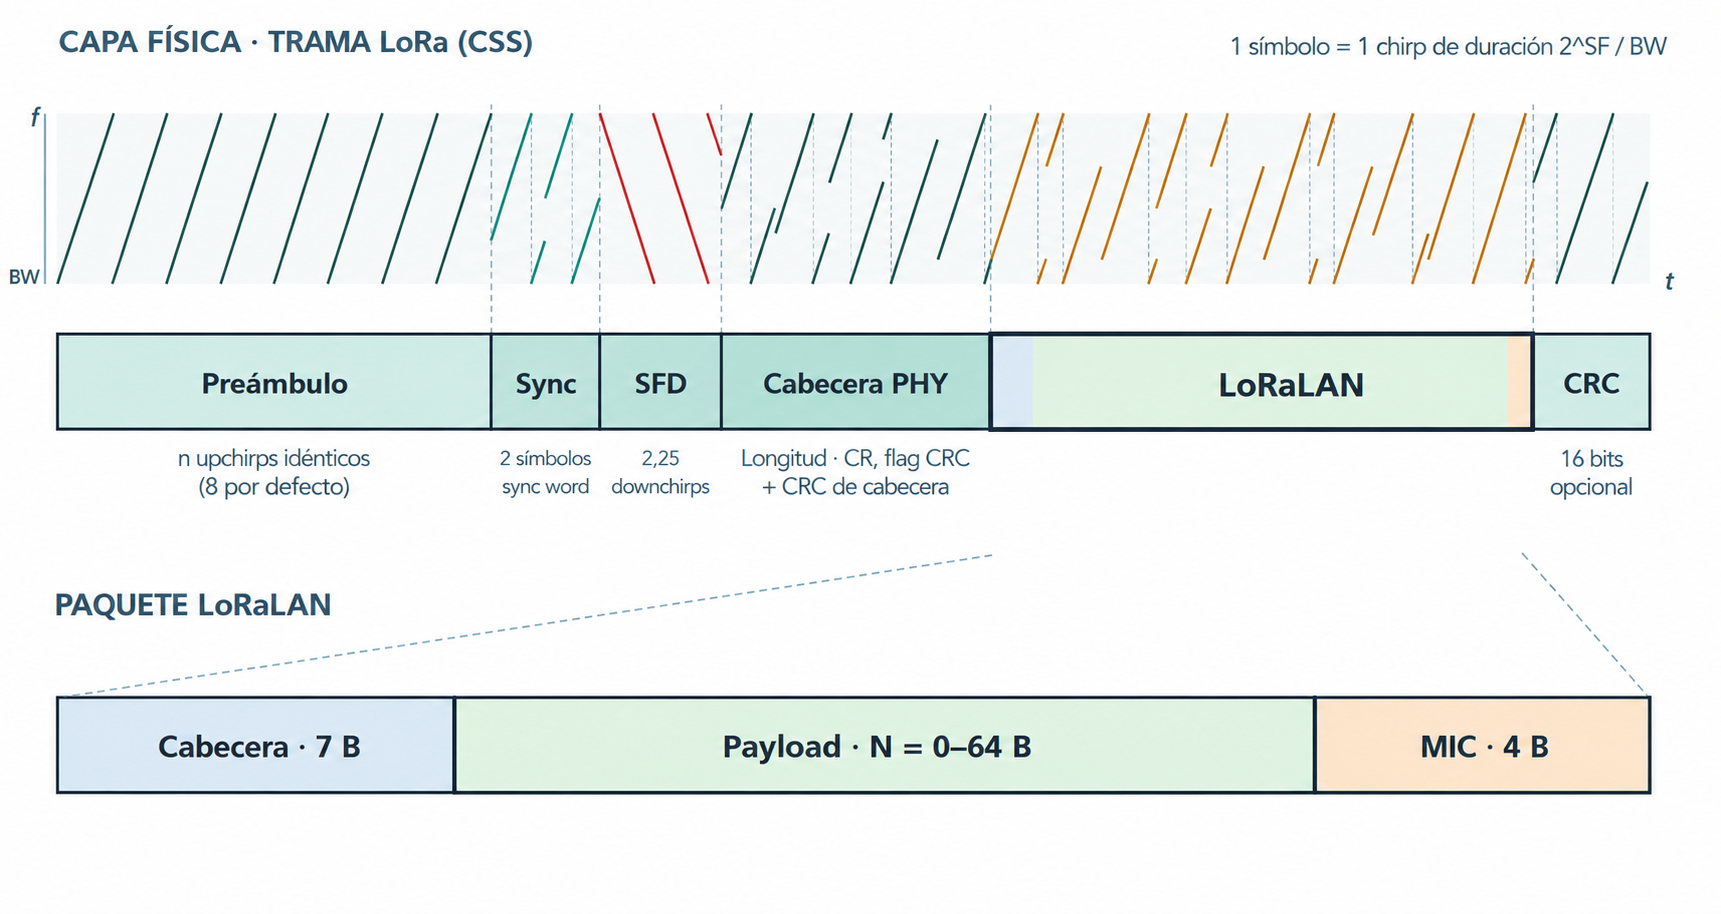
\includegraphics[width=1\linewidth]{./imagenes/loralanDentroLora.png}
    \caption{Encapsulación de paquete LoRaLAN dentro de la trama LoRa. }
    \label{fig:loralanDentroLora}
\end{figure}

\subsection{Cabecera}

En la figura~\ref{fig:loralancabecera} se muestra el formato del paquete y se desglosa la cabecera que llevan los paquetes tal y como viajan por el aire.

\begin{figure}[h]
    \centering
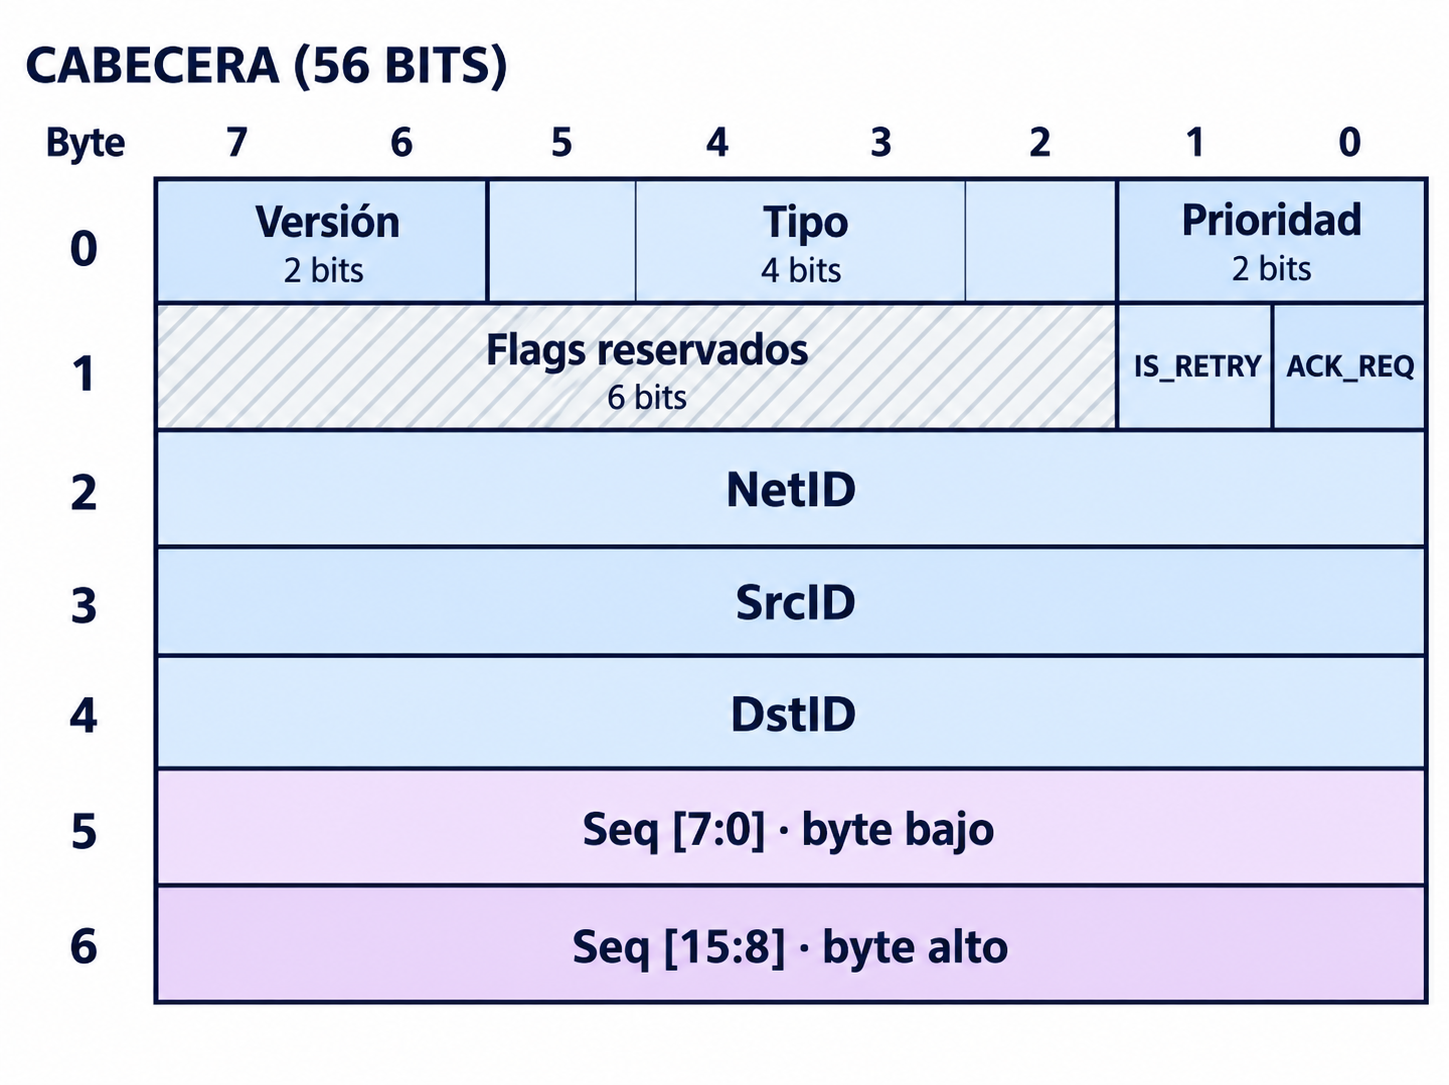
\includegraphics[width=0.8\linewidth]{./imagenes/cabecera.png}
    \caption{Campos de la cabecera de paquete LoRaLAN. }
    \label{fig:loralancabecera}
\end{figure}

En primer lugar se reservan 2 bits para indicar la \textbf{versión del protocolo} que se está utilizando. De esta forma, se permite que el protocolo pueda mejorarse y que puedan existir hasta cuatro versiones con distintas propiedades en un futuro.

El siguiente campo que aparece es el campo \textbf{tipo}, al que se asignan 4 bits. Este campo indica qué tipo de paquete se envía. Puede haber hasta 16 tipos de paquetes, aunque hasta el momento solo se han definido nueve.

Los nueve tipos de mensaje definidos, que se muestran en la Tabla~\ref{tab:tipos}, cubren el ciclo de vida completo de la red.
\begin{table}[H]
\centering
\caption{\label{tab:tipos} Tipos de mensaje de LoRaLAN.}
\small
\begin{tabular}{|c|l|p{8.5cm}|}
\hline
\textbf{Cód.} & \textbf{Tipo} & \textbf{Descripción} \\
\hline
\texttt{0x01} & PUSH\_EVENT & Evento de aplicación, el nodo lo envía por iniciativa propia al gateway. \\
\hline
\texttt{0x02} & ACK & Confirmación de recepción de un paquete, que puede llevar código de confirmación dentro del propio paquete. \\
\hline
\texttt{0x03} & POLL & Sondeo periódico que emite el gateway preguntando a un nodo si tiene datos que enviarle. \\
\hline
\texttt{0x04} & POLL\_RESPONSE & Respuesta del nodo a un sondeo, con los datos de aplicación que tuviera pendientes. \\
\hline
\texttt{0x06} & TIME\_SYNC & Difusión de la hora del gateway para que los nodos sincronicen su reloj. \\
\hline
\texttt{0x07} & JOIN\_REQUEST & Solicitud de un nodo para asociarse a una red. \\
\hline
\texttt{0x08} & JOIN\_ACCEPT & Respuesta del gateway a la solicitud de asociación, con el identificador asignado al nodo. \\
\hline
\texttt{0x09} & LEAVE & Aviso del nodo de que abandona la red. \\
\hline
\texttt{0x0A} & CMD & Orden que el gateway envía a un nodo por iniciativa propia. \\
\hline
\end{tabular}
\end{table}


El código \texttt{0x05} está reservado, debido a que correspondía a un mensaje de descubrimiento sin claves (HELLO) de las primeras versiones, que se eliminó cuando su función quedó cubierta por la asociación autenticada. 

Cabe destacar que el ACK reutiliza el campo de secuencia con un significado distinto al del resto de tramas: no lleva un número propio, sino el de la trama que confirma, permitiendo al emisor emparejar cada confirmación con su envío.

El siguiente campo que aparece es el de \textbf{prioridad}. Para este campo se reservan 2 bits, con los que se completa el primer byte de la cabecera.

El campo Prioridad puede tomar los valores de prioridad baja (0), media (1) y alta (2). Actualmente es solo informativo.

A continuación, aparece el campo \textbf{Flags}. Este campo ocupa un byte, aunque actualmente solo utiliza los bits ACK\_REQUIRED e IS\_RETRY. Esta decisión mantiene la cabecera alineada a byte sin reducir el espacio destinado a tipos o prioridades. El coste adicional de mantener este byte es mínimo, mientras que los seis bits restantes quedan reservados para futuras extensiones. Estos deben permanecer a cero y cualquier trama que incumpla esta condición será descartada, de modo que la incorporación de nuevos indicadores requerirá implementar una nueva versión del protocolo.

El indicador ACK\_REQUIRED señala al receptor que debe confirmar el paquete con un ACK. Por otro lado, el indicador IS\_RETRY señala que el paquete es una retransmisión. Este bit es solo informativo ya que se puede deducir que es una retransmisión por el número de secuencia.  

El siguiente byte representa el \textbf{identificador de red}. Como su nombre indica, sirve para separar redes que funcionan en el mismo canal. Si un nodo recibe un paquete con un netId distinto al de su red, lo descarta.

Los siguientes bytes representan la \textbf{dirección de origen} y la \textbf{dirección de destino} de los paquetes. Esto quiere decir que se dispone de un total de 254 direcciones para nodos, ya que la dirección 255 (0xFF) corresponde a la dirección de broadcast y la dirección 0 (0x00) corresponde a la dirección del gateway. Aunque teóricamente 254 sería el máximo de nodos que podrían conectarse a la red, dicho máximo se reduce a las 32 entradas de la tabla de direcciones que puede mantener el gateway. Este valor resulta adecuado para la aplicación del caso de uso y, además, disminuye el tiempo que tarda el gateway en sondear a todos los nodos y reduce su ciclo de trabajo.

Por último, se dedican dos bytes al \textbf{número de secuencia}, que cada emisor incrementa en cada envío. Permite al receptor descartar duplicados y repeticiones. Al emisor le permite emparejar cada ACK con su envío, ya que el ACK devuelve el número de la trama que confirma. Se emplean 16~bits porque, con un solo byte, el contador daría la vuelta cada 256~tramas y una trama capturada volvería a parecer nueva al poco tiempo.

Respecto a los duplicados, una retransmisión llega al receptor cuando la trama original también llegó pero su ACK se perdió. El receptor detecta el duplicado por el número de secuencia y, en ese caso, no entrega los datos a la aplicación por segunda vez, pero sí vuelve a confirmar. Esto se aplica tanto en el gateway, con los eventos y las respuestas de sondeo, como en el nodo, con las órdenes.

\subsubsection{Carga útil y código de integridad (MIC)}

La carga útil se limita a 64~bytes, lo que mantiene un equilibrio entre capacidad y tiempo en el aire. Con SF7, 125~kHz, CR 4/5, 8~símbolos de preámbulo, cabecera explícita y CRC, el paquete máximo (75~bytes) ocupa el canal 133~ms y el mínimo (11~bytes), 41~ms, según las fórmulas de Semtech recogidas en el Anexo~\ref{anexo:toa}. En esta versión inicial se descarta aplicar fragmentación de paquetes.

Tras el último byte de datos se incluye el MIC (\emph{Message Integrity Code}), un código de cuatro bytes, obtenido con CMAC-AES-128\cite{rfc4493}, que cubre la cabecera completa y la carga útil cifrada en los mensajes que transportan datos de aplicación y en claro en el resto. Su cálculo requiere una clave que depende del interlocutor, como se detalla en el apartado~\ref{sec:integridad}.

Antes de cualquier otra comprobación, el receptor comprueba que el paquete esté bien formado, es decir, que su longitud esté entre 11 y 75~bytes, que la versión sea la vigente, que el tipo esté definido, que la prioridad sea válida y que los indicadores reservados estén a cero, y descarta la trama que no supere alguna de estas comprobaciones. La cabecera no incluye un campo de longitud, ya que la cabecera explícita de LoRa transporta la longitud de la carga protegida por su propio CRC, de modo que la longitud de los datos de aplicación se deduce de la longitud total recibida. Un paquete alterado en tránsito para alargarlo o recortarlo puede superar esta validación estructural, pero no la del MIC, puesto que el cambio de longitud altera los bytes cubiertos y la posición del propio código. 

Mediante el MIC se garantizan la integridad y la autenticidad del paquete, lo que permite descartar los paquetes que presentan modificaciones no autorizadas y verificar que el emisor es legítimo y posee la clave secreta.
\section{Gestión del direccionamiento y vinculación a redes}\label{sec:join}


\subsection{Asociación (JOIN)}

La asociación es el mecanismo mediante el cual un nodo se vincula a una red LoRaLAN para poder transmitir información y posee tres funciones: autenticar al nodo y al gateway mediante una clave maestra precompartida (denominada \textit{APPKEY}, de 128~bits), establecer una clave de sesión exclusiva de ese nodo y dar de alta al nodo en la tabla del gateway. Los pasos que se llevan a cabo son los siguientes:

\begin{enumerate}
\item El nodo genera un número aleatorio de 16~bits, denominado \textit{DevNonce}, y emite un paquete tipo JOIN\_REQUEST a la dirección de difusión con su tipo de dispositivo, dicho DevNonce y su identificador de fábrica (dirección MAC), empleando como dirección de origen la que desea obtener. Este paquete se autentica con la clave APPKEY.

\item El gateway verifica el MIC, localiza al nodo en su tabla por su identificador de fábrica o le asigna una dirección si no figura en ella, y deriva la clave de sesión a partir de la dirección asignada. Posteriormente, responde con un JOIN\_ACCEPT dirigido a esa dirección, que contiene la propia dirección asignada, el mismo DevNonce, un código de estado y el identificador de fábrica del nodo.

\item El nodo comprueba que el DevNonce y el identificador de fábrica devueltos coinciden con los suyos, lo que liga la respuesta a su petición, adopta la dirección asignada y deriva la misma clave por su cuenta. Finalmente, confirma con un ACK que ya va autenticado con la clave de sesión.
\end{enumerate}
 
De esta forma, la clave de sesión no viaja nunca por el aire, sino que en ambos extremos se calcula a partir de datos de los que se dispone. Si no recibe respuesta, el nodo repite la petición cada 5~segundos (valor configurable), con un DevNonce nuevo en cada intento. Para emitir un paquete JOIN\_REQUEST se realiza previamente una escucha del canal y, si este se encuentra ocupado, el intento se aplaza al siguiente periodo.

Cuando un nodo previamente asociado se reinicia, vuelve a solicitar la asociación. El gateway la acepta, deriva una clave nueva y reinicia el estado de esa sesión, incluido el control de secuencia. 

Si el gateway se reinicia, su tabla arranca vacía y deja de reconocer a los nodos que siguen considerándose asociados, de modo que descarta sus paquetes, por no disponer de su clave de sesión, y no los incluye en el sondeo. Para detectar esta situación, el nodo registra el instante del último paquete recibido con su clave de sesión (POLL, CMD o ACK) y, si transcurre un plazo (configurable) sin recibir ningún paquete destinado a él, da la sesión por perdida, borra su clave y vuelve a solicitar la asociación. Los paquetes TIME\_SYNC no se tienen en cuenta, puesto que se autentican con la clave maestra y un gateway reiniciado los sigue emitiendo. Dicho plazo debe superar, al menos, una vuelta completa de sondeo, cuya duración depende del número de nodos asociados.

\subsection{Asignación dinámica de direcciones}\label{sec:direcciones}

Cada nodo dispone de un \textbf{identificador de fábrica} de 6~bytes, la dirección MAC grabada en el microcontrolador, que viaja en el JOIN\_REQUEST y en el JOIN\_ACCEPT. Conviene no confundirlo con el DevNonce, cuyo papel es distinto. El identificador de fábrica es fijo y señala quién es el nodo, mientras que el DevNonce cambia en cada intento, lo que impide repetir una asociación capturada y garantiza que cada sesión tenga una clave distinta. Que el JOIN\_ACCEPT incluya también el identificador permite a cada nodo reconocer la respuesta que le corresponde aunque varios se asocien a la vez, como ocurre tras un corte de suministro general, por ejemplo.

Al recibir una petición, el gateway asigna la dirección aplicando las siguientes reglas, en este orden:

\begin{enumerate}
\item Si el identificador de fábrica ya figura en su tabla, devuelve la misma dirección, sea cual sea la que pida el nodo.

\item En caso contrario, concede la dirección que el nodo solicita como origen del JOIN\_REQUEST, siempre que no sea \texttt{0x00} (por defecto, sin preferencia), \texttt{0xFF} ni la del propio gateway y que no la ocupe otro nodo.

\item Si no puede concederla, asigna la dirección libre más alta, empezando por la 254. Si no queda ninguna, la petición se rechaza.
\end{enumerate}

La tabla de direcciones del gateway reside en memoria durante la ejecución, de modo que la persistencia la aporta el nodo, que guarda la dirección recibida en su memoria no volátil y la solicita de nuevo en cada asociación. La biblioteca se limita a ofrecer la dirección preferida como parámetro de configuración y la asignada como dato consultable, por lo que su almacenamiento se delega en la capa de aplicación. Con este reparto, un nodo recupera su dirección tanto si se reinicia el gateway, ya que la conserva en memoria y la pide al reasociarse, como si se produce un corte general, puesto que la lee de su memoria no volátil.

El protocolo ofrece un direccionamiento dinámico similar al que ofrece DHCP. Se aplica ofreciendo al nodo la dirección más alta disponible. De esta manera se reservan las direcciones bajas (1-127) para direccionamiento fijo. Es decir, los administradores de la red pueden asignar a un nodo una dirección de ese rango, de manera que el gateway le proporcionará al nodo la dirección deseada si se encuentra disponible.


\subsection{Baja (LEAVE)}

Un nodo abandona la red emitiendo un paquete LEAVE y esperando el ACK correspondiente. Tras recibirlo, borra su clave de sesión y deja de intentar asociarse hasta que su aplicación lo solicite. Si tras varias repeticiones no se recibe ACK, el nodo abandona la red de igual forma. La pérdida del LEAVE o de su ACK no deja a la red en un estado incoherente, ya que el gateway registra el instante del último paquete recibido de cada nodo y, si este no responde tras varias ventanas de sondeo, lo marca como inactivo.

Un nodo puede desaparecer porque se ha dado de baja, porque se ha apagado o porque ha quedado fuera de cobertura. En cualquiera de estos casos deja de responder a los sondeos y la aplicación puede considerarlo inactivo. No obstante, el gateway no lo retira por sí mismo del turno de sondeo, de modo que un nodo que desaparece sin que su baja llegue al gateway sigue consumiendo su turno para que pueda recuperarse si su ausencia es temporal.

\section{Acceso al medio híbrido}\label{sec:mac}

LoRaLAN aplica un esquema híbrido con dos modos complementarios, en línea con los trabajos sobre coordinación centralizada y escucha previa del canal revisados en el Capítulo~\ref{chap:2}.

\subsubsection{Modo POLL o sondeo dirigido por el gateway}\label{sec:poll}

El gateway recorre cíclicamente su tabla de nodos asociados y asigna un periodo de tiempo configurable que determina cuánto tiempo pasa entre que se consulta a un nodo y a otro. Para ello, cuando a un nodo le llega su turno, el gateway envía un POLL\_REQUEST a dicho nodo. El nodo interrogado contesta con un POLL\_RESPONSE, cuyo contenido se elige en el siguiente orden:

\begin{enumerate}
    
\item Los datos que la aplicación hubiera dejado preparados para el siguiente sondeo, o los de un evento cuya entrega por el modo PUSH no se confirmó, si los hay.

\item Datos que la aplicación genera en ese instante, si se registra una función para ello (sondeo bajo demanda). En el caso de uso de este trabajo se aplica a telemetría proporcionada por lectura de sensores y estado de relés.

\item En último lugar, una carga vacía, que sirve como señal de vida (Heartbeat).

\end{enumerate}

El POLL\_REQUEST no requiere confirmación, puesto que el propio POLL\_RESPONSE ya sirve como acuse de recibo. Por otro lado, la confirmación del POLL\_RESPONSE será necesaria o no, dependiendo de su contenido. Las respuestas vacías y las generadas bajo demanda, que transportan telemetría o estado que el siguiente sondeo vuelve a refrescar, se emiten una sola vez y sin confirmación, de modo que el ciclo habitual consta únicamente de dos paquetes: el POLL\_REQUEST y el POLL\_RESPONSE.

Por el contrario, los datos prioritarios se envían como una transmisión fiable que el gateway confirma, salvo que la aplicación indique lo contrario al encolarlos. El ciclo consta en ese caso de tres paquetes. El nodo retransmite la respuesta si la confirmación no llega y conserva los datos hasta recibirla, de manera que, si agota los intentos, los vuelve a enviar en el siguiente turno de sondeo.

Que el gateway elija el turno de cada nodo resulta la vía más eficiente para el tráfico rutinario, como la telemetría o el estado. Su principal desventaja es la latencia. Dados $N$ nodos y un intervalo de sondeo $T_{poll}$, cada nodo es interrogado cada $N \cdot T_{poll}$. Como el gateway emite un POLL en cada intervalo, $T_{poll}$ es el parámetro que fija el consumo de ciclo de trabajo del gateway y debe elegirse teniendo en cuenta dicho criterio.


\subsubsection{Modo PUSH: eventos asíncronos con CAD}

Un evento que no puede esperar a su turno, como un registro de asistencia, se transmite como PUSH\_EVENT. Para no interferir con una transmisión en curso de otro nodo o del gateway, el nodo escucha previamente el canal mediante la detección de actividad (CAD) del transceptor. El CAD está implementado por hardware en el transceptor LoRa utilizado, el SX1276 \cite{semtech_sx1276}. Con este diseño, se pueden dar tres casos:

\begin{enumerate}
\item Si el canal está \textbf{libre}, emite su transmisión.
\item Si el canal se encuentra \textbf{ocupado}, aplaza el intento aplicando un tiempo de retroceso (\textit{backoff}) exponencial con una componente aleatoria:
\begin{equation}\label{eq:backoff}
t_{espera} = t_{base} \cdot 2^{\min(k,\;k_{max})} + U(0,\;t_{jitter})
\end{equation}
donde $k$ es el número de escuchas fallidas del evento y $U$ una variable uniforme. Con los valores por defecto ($t_{base}=40$~ms, $k_{max}=5$, $t_{jitter}=50$~ms), la espera crece desde 80~ms hasta unos 1,3~s, y la componente aleatoria evita que dos nodos que han detectado la misma trama reintenten a la vez.

\item Si la escucha falla por un error de la radio, reintenta tras una espera fija y corta, de 60~ms.
\end{enumerate}

Un nodo mantiene un único evento pendiente de entrega. La aplicación no puede encolar otro evento hasta que el anterior se haya transmitido. Mientras existe una transmisión propia a la espera de confirmación, el nodo no realiza escuchas, dado que el CAD saca momentáneamente a la radio del modo de recepción y podría hacerle perder precisamente la confirmación que espera.


La escucha previa del canal se aplica \textbf{únicamente en los nodos} y solo a la primera emisión de cada PUSH\_EVENT y a cada JOIN\_REQUEST; si el canal está ocupado, el evento aplica el retroceso descrito y el JOIN espera a su siguiente intento. Las retransmisiones y el resto de tramas del nodo, así como todas las del gateway, se emiten sin escuchar.

Esta decisión es coherente con el rol del gateway como coordinador, puesto que es el único origen del tráfico descendente y él mismo provoca el ascendente del sondeo. Se entiende como tráfico ascendente (Uplink) a aquellos paquetes que van del nodo al gateway y descendente (Downlink) al tráfico que va desde el gateway a los nodos.

En contrapartida, un PUSH\_EVENT puede estar en el aire cuando el gateway emite un POLL o un TIME\_SYNC, en cuyo caso pueden perderse una o ambas tramas. Los reintentos permiten resolver las colisiones.

Aunque en esta versión el campo prioridad es informativo, los paquetes de tipo evento, confirmaciones y órdenes llevan un valor de prioridad alto, los paquetes relativos al sondeo una prioridad baja y prioridad media para paquetes que tratan la gestión de red (asociación, baja y sincronización). Esta decisión se hereda de una versión anterior en la que se planteaba que el gateway pudiera usar un planificador de colas para gestionar el tráfico de la red, como haría un switch o router para mantener la calidad del servicio (QoS).


\section{Fiabilidad}\label{sec:fiabilidad}

Los paquetes que llevan activado el indicador de confirmación requerida deben ser contestados con un ACK. El emisor aplica un esquema de parada y espera (\textit{stop-and-wait}): transmite el paquete, espera el ACK durante un plazo de 1200~ms por defecto y, si este no llega, retransmite hasta alcanzar un máximo de tres intentos en total. Cada retransmisión conserva el número de secuencia original y activa el indicador de retransmisión, lo que modifica la cabecera y obliga a recalcular el MIC. Cada dispositivo mantiene una única transmisión fiable en curso, mientras que las tramas que no piden confirmación se emiten una sola vez, sin esperar ningún ACK.

También se aplica otro mecanismo más simple. Si el transceptor informa de un fallo al transmitir, el envío se repite tras una pausa aleatoria de 30 a 180~ms, hasta tres veces, salvo en paquetes que no piden confirmación, que se intentan una única vez.

Respecto a los duplicados, una retransmisión llega al receptor cuando la trama original también llegó pero su ACK se perdió. El gateway detecta el duplicado por el número de secuencia y, en ese caso, \emph{no entrega los datos a la aplicación por segunda vez, pero sí vuelve a confirmar}.

Por otro lado, un PUSH\_EVENT podría agotar sus retransmisiones sin recibir confirmación. En ese caso, si la aplicación lo solicitó, sus datos no se descartan, sino que se guardan como carga del siguiente POLL\_RESPONSE, de modo que el evento pierde su carácter inmediato pero se garantiza su entrega en cuanto el gateway vuelve a interrogar al nodo. Dado que el gateway pudo recibir el evento original aunque se perdieran todas sus confirmaciones, los datos rescatados pueden llegar duplicados con otro número de secuencia, por lo que la aplicación debe reconocerlos por cualquiera de las dos vías y tolerar esa repetición.

Tanto si la confirmación llega como si se agotan los intentos, el nodo notifica a su aplicación el desenlace de cada evento, siendo esta la que decide qué hacer: mostrar un error, guardar el dato para más tarde o descartarlo.

Estos mecanismos presentan algunas limitaciones, puesto que ciertos conflictos, como los duplicados que puede generar el rescate por sondeo, se delegan en la capa de aplicación, y en otros casos la entrega no se pierde, pero se retrasa. Así, dado que cada dispositivo mantiene un único envío fiable en curso, los datos preparados que requieren confirmación no pueden salir en un sondeo que llegue mientras el nodo espera otro ACK, pero no se descartan, sino que se conservan para el sondeo siguiente.

\subsubsection{Confirmación con carga útil (ACK diferido)}\label{sec:ackdiferido}

Se han realizado algunas modificaciones pensando en el caso de uso. En este caso, cuando el nodo envía la tarjeta leída para procesar un fichaje, debe indicar al nodo si el fichaje se ha registrado correctamente o se ha rechazado, y además por qué. Esta decisión la toma el servidor.

Para cubrir esta necessidad se decide que la respuesta de la aplicación viaja dentro del propio ACK.

Cuando el gateway se configura con confirmación diferida, la recepción de un PUSH\_EVENT no genera el ACK automático. En su lugar, el protocolo entrega el evento a la aplicación del gateway y deja la confirmación en suspenso. Una vez que la aplicación dispone de la respuesta, la entrega al protocolo junto con el identificador del nodo y el número de secuencia del evento, y el protocolo emite el ACK con esa respuesta como carga útil. En el nodo la respuesta llega a la aplicación junto con el resultado del envío.

Para que este mecanismo sea compatible con los reintentos, el gateway guarda, por cada nodo, el estado de la confirmación de su último evento, que puede tomar tres valores:

\begin{itemize}
\item \textbf{Pendiente}: El evento se ha entregado a la aplicación y esta aún no ha respondido. Si llega una retransmisión del mismo evento, el gateway no contesta, ya que todavía no dispone de respuesta y el nodo volverá a intentarlo.
\item \textbf{Lista}: La aplicación ha respondido y el ACK se ha emitido. Además, el gateway \emph{conserva la respuesta}, de modo que si el ACK se pierde y el nodo retransmite, este recibe la misma respuesta sin que la aplicación vuelva a ser consultada.
\item \textbf{Ninguna}: No hay ningún evento en curso para ese nodo.
\end{itemize}

De este modo, un evento se procesa una sola vez aunque se transmita varias, y todas sus retransmisiones obtienen la misma respuesta. Si la aplicación entrega una respuesta cuando el evento ya no está pendiente (porque ha llegado otro posterior o porque el nodo se ha reasociado), dicha respuesta se rechaza.

%pero esto podría dar lugar a que no se envie la confirmación...

La respuesta debe emitirse antes de que venza el plazo de espera del nodo, que es de 1200~ms por defecto. El protocolo no impone cómo se consigue, de modo que es responsabilidad de la aplicación del gateway responder a tiempo, aunque sea con una respuesta provisional. En el Capítulo~\ref{chap:7} se describe cómo lo resuelve el sistema de fichaje.

Como alternativa a este mecanismo, se podría haber definido una confirmación negativa (NACK). Esta opción se descartó, ya que la distinción entre «aceptado» y «rechazado» pertenece a la aplicación, por lo que el protocolo debe transportar la respuesta sin interpretarla.

Otro detalle que cabe destacar es que la carga del ACK no se cifra, aunque el MIC, calculado con la clave de sesión, garantiza que procede del gateway y que no se ha alterado. Como cualquiera que escuche el canal tiene capacidad de leerla, no debe emplearse para datos confidenciales, sino para códigos de resultado breves.



\subsubsection{Sincronización temporal}

% REVISAR LA HORA PQ ES COMPLICADO PARA CREAR UNA HORA
El gateway difunde, con la periodicidad que indique el programador, un paquete TIME\_SYNC con una marca de tiempo de 32~bits en segundos, a partir de la cual cada nodo calcula y almacena su desfase respecto al reloj local sin modificarlo, de modo que la aplicación puede consultarlo para fechar sus datos o mostrar la hora. Este mecanismo es un servicio para la aplicación y no interviene en el acceso al medio, puesto que el sondeo de LoRaLAN es de pregunta y respuesta y un nodo transmite al recibir su POLL y no según su reloj, por lo que la pérdida de tramas TIME\_SYNC no afecta al funcionamiento de la red. Su resolución es de un segundo, ya que no tiene en cuenta el tiempo en el aire de la trama, y el valor difundido es el tiempo de funcionamiento del gateway y no la hora del día, cuya difusión exigiría ampliar la aritmética del nodo, que opera con milisegundos en 32~bits. Al tratarse de una trama de difusión, se autentica con la clave maestra, que es la única que comparten todos los nodos.

\section{Arquitectura de seguridad}\label{sec:seguridad}

El diseño de la seguridad asume de base que el canal es hostil \cite{chacko2018security}, puesto que cualquiera con un receptor LoRa en la misma frecuencia puede escuchar, capturar y reinyectar tramas LoRa. Se decide aprovechar el motor de aceleración hardware que ofrece el ESP32 \cite{babiuch2019esp32}, en dos modos: el modo contador para cifrar la carga útil con el algoritmo AES-128 y CMAC para autenticar paquetes y derivar las claves de sesión.

\subsubsection{Confidencialidad}

La carga útil de los paquetes que transportan datos de aplicación (PUSH\_EVENT, POLL\_RESPONSE y CMD) se cifra con AES-128 en modo contador (CTR) \cite{nist80038a} bajo la clave de sesión del nodo. Se ha elegido este modo porque convierte el cifrador de bloque en uno de flujo, de manera que el texto cifrado ocupa lo mismo que el original y la trama no crece, en coherencia con el primer principio de diseño.

%REVISAR SI EL NODO USA LA CLAVE DE NODO O LA CLAVE PRECOMPARTIDA.
El bloque inicial del contador se forma con el identificador de red, la dirección del emisor y el número de secuencia. La dirección del emisor es necesaria porque los dos sentidos del enlace comparten clave, y sin ella una trama del gateway y otra del nodo con el mismo número de secuencia emplearían el mismo flujo de cifrado.

El resto viaja en claro. La cabecera no puede cifrarse, ya que el receptor necesita leer el identificador de red y las direcciones para saber si la trama le concierne y con qué clave verificarla, y tampoco se cifran las tramas de gestión ni la carga del ACK, que solo contienen datos de control.

\subsubsection{Integridad y autenticidad}\label{sec:integridad}

El MIC ya descrito se calcula sobre la carga ya cifrada, de modo que el receptor lo verifica antes de descifrar y descarta cualquier trama que no lo supere sin llegar a procesarla (esquema \textit{Encrypt-then-MAC}). Con 4~bytes, el mismo tamaño que emplea LoRaWAN, la probabilidad de que una trama falsificada al azar sea aceptada es de $2^{-32}$, y cada intento le cuesta al atacante una transmisión completa.

La clave con la que se calcula depende del tipo de trama. Las de asociación usan la clave maestra, porque todavía no existe clave de sesión, y también la usa TIME\_SYNC, porque al difundirse a todos los nodos necesita una clave que todos compartan. El resto de tramas se autentica con la clave de sesión del nodo que interviene, por lo que el MIC se calcula en el momento de transmitir y no al construir la trama, y si no existe clave para el interlocutor, la trama no se emite ni se acepta.

\subsubsection{Derivación de claves de sesión}\label{sec:kdf}

La clave de sesión se obtiene durante la asociación aplicando CMAC con la clave maestra sobre una etiqueta fija, el identificador de red, la dirección asignada al nodo y el DevNonce:

\begin{equation}
K_{sesion} = \mathrm{CMAC}_{APPKEY}\big(\,\texttt{LLK} \parallel id_{red} \parallel id_{nodo} \parallel DevNonce\,\big)
\end{equation}

Al intervenir la dirección y el DevNonce, cada nodo tiene una clave distinta que además cambia en cada asociación, y como CMAC no es reversible, conocer la clave de un nodo no permite deducir la de otro ni la clave maestra. La etiqueta fija evita que la entrada de la derivación pueda coincidir con la de una trama de asociación autenticada con la misma clave. La primera versión del protocolo no cumplía esta propiedad, ya que derivaba las claves con una función lineal, se sustituyó para que fuera más robusta.

\subsubsection{Protección frente a repetición}\label{sec:antirepeticion}

Un paquete capturado y reinyectado sin modificar conserva un MIC válido, por lo que solo puede rechazarse si el receptor recuerda qué números de secuencia ha aceptado ya. Para ello, cada receptor guarda, por cada interlocutor, el último número aceptado y un mapa de 64~bits que indica cuáles de los 64~números anteriores ha recibido. Una paquete se acepta solo en alguno de estos dos casos:

\begin{itemize}
\item Si su número avanza respecto al último aceptado hasta media escala, es decir, entre 1 y 32\,767~posiciones teniendo en cuenta la vuelta del contador. En ese caso pasa a ser el último aceptado y el mapa se desplaza.

\item Si es uno de los 64~números anteriores y el mapa indica que todavía no se ha recibido, lo que permite aceptar tramas que llegan fuera de orden.
\end{itemize}

Cualquier otro número se considera una repetición o una trama demasiado antigua y se rechaza. Admitir avances de hasta media escala permite recuperar la comunicación tras una racha larga de pérdidas y, al mismo tiempo, distinguir sin ambigüedad una trama nueva de una antigua cuando el contador da la vuelta. El esquema es análogo a la ventana antirrepetición que usa IPsec \cite{rfc4303}.

El filtro se aplica en los dos extremos. El gateway lo aplica a las tramas PUSH\_EVENT y POLL\_RESPONSE de cada nodo, y el nodo, a las que recibe del gateway con su clave de sesión, de modo que una orden capturada y reinyectada no vuelve a ejecutarse. El ACK queda fuera, ya que no lleva un número propio, sino el de la trama que confirma. El estado se reinicia en cada asociación, de modo que un nodo que se reinicia y vuelve a contar desde cero no queda bloqueado.

%Pero si se reinicia no va a saber continuar la comun. A nada coño q emite join de nuevo es verdad

Ese reinicio abriría una vía de ataque si bastase con reinyectar un JOIN\_REQUEST capturado para reiniciar la sesión y, con ella, el filtro de secuencia. Por ello el gateway rechaza la petición de un nodo asociado que repita el último DevNonce aceptado, lo que no afecta a los reintentos legítimos, que generan un DevNonce nuevo en cada intento.

Una retransmisión legítima es indistinguible de una repetición maliciosa, y el protocolo trata ambas del mismo modo: no entrega los datos otra vez a la aplicación, pero sí vuelve a enviar el ACK. Así, un nodo que recibe de nuevo una orden ya ejecutada, porque se perdió su confirmación, la confirma sin ejecutarla otra vez, y lo único que consigue un atacante es provocar una confirmación.

El identificador de red, por su parte, separa despliegues vecinos, pero no es un mecanismo de seguridad, ya que viaja en claro. Lo que aísla realmente dos redes es que tengan claves maestras distintas.

\subsubsection{Limitaciones conocidas}\label{sec:limitaciones-seg}

Los mecanismos anteriores protegen frente a la escucha, la falsificación y la repetición de los datos que los nodos envían al gateway, aunque permanecen abiertas las siguientes limitaciones:


% REVISAR SI ESTO ES 100% VERDAD
\begin{enumerate}
\item \textbf{Sin renovación de clave}: La clave solo cambia al reasociarse. Cuando un emisor supera las 65\,536~tramas en una misma sesión, se repite el bloque inicial del contador, lo que permitiría combinar dos textos cifrados para obtener información de los originales. Además, una trama capturada vuelve a parecer nueva en cuanto el contador ha avanzado más de media escala desde ella. 

\item \textbf{TIME\_SYNC no se filtra}: Un atacante puede reinyectar una TIME\_SYNC antigua y alterar el desfase de reloj que calculan los nodos. El efecto es bastante limitado y afecta a la hora que consulta la aplicación, ya que esta trama no interviene en el acceso al medio ni cuenta como señal de vida.

\item \textbf{Repetición de una asociación antigua}: El gateway solo recuerda el último DevNonce de cada nodo, de modo que un JOIN\_REQUEST más antiguo le hace derivar una clave que el nodo ya no usa, y este queda incomunicado hasta que se reasocia.

\item \textbf{Clave maestra compartida}: Todos los dispositivos guardan la misma clave maestra, por lo que extraerla de uno de ellos compromete la red entera, ya que permite derivar las claves de sesión de las asociaciones observadas, falsificar tramas de difusión y suplantar el identificador de fábrica de cualquier nodo. 

\item \textbf{Metadatos y disponibilidad}: La cabecera, los paquetes de gestión y los ACK son legibles, por lo que un observador sabe qué nodos existen y cuándo transmiten, y nada protege frente a la interferencia deliberada del canal.
\end{enumerate}

\section{Máquinas de estados}

El comportamiento del protocolo se resume en dos máquinas de estados, una por cada rol.

\subsection{Nodo}

El nodo se encuentra en uno de los cuatro estados que se muestran en la Tabla~\ref{tab:fsm-nodo}.

\begin{table}[H]
\centering
\caption{\label{tab:fsm-nodo} Máquina de estados del nodo.}
\begin{tabular}{|p{2.9cm}|p{4.7cm}|p{6.0cm}|}
\hline
\textbf{Estado} & \textbf{Suceso} & \textbf{Acción y estado siguiente} \\
\hline
\multirow{2}{2.9cm}{No asociado}
 & Vence el periodo de asociación & CAD; si libre, JOIN\_REQUEST con DevNonce nuevo. Sigue no asociado. \\
\cline{2-3}
 & JOIN\_ACCEPT válido & Deriva la clave, envía ACK $\rightarrow$ En reposo. \\
\hline
\multirow{6}{2.9cm}{En reposo (asociado, en recepción)}
 & POLL & Envía POLL\_RESPONSE $\rightarrow$ Esperando ACK. \\
\cline{2-3}
 & CMD & Si la secuencia es nueva, descifra y entrega a la aplicación; en todo caso, envía ACK. \\
 \cline{2-3}
 & TIME\_SYNC & Actualiza el desfase de reloj. \\
\cline{2-3}
 & La aplicación encola un evento & $\rightarrow$ Evento pendiente. \\
\cline{2-3}
 & La aplicación pide la baja & Envía LEAVE, borra la clave $\rightarrow$ No asociado (sin reintento automático). \\
\cline{2-3}
 & Vence el plazo de silencio sin POLL, CMD ni ACK & Borra la clave y conserva su dirección $\rightarrow$ No asociado (con reintento automático). \\
\hline
\multirow{2}{2.9cm}{Evento pendiente}
 & CAD libre & Envía PUSH\_EVENT $\rightarrow$ Esperando ACK (o En reposo, si no pide confirmación). \\
\cline{2-3}
 & CAD ocupado o con error & Programa el retroceso (ec.~\ref{eq:backoff}). Sigue pendiente. \\
\hline
\multirow{3}{2.9cm}{Esperando ACK}
 & ACK con la secuencia esperada & Notifica entrega (y respuesta, si la trae) $\rightarrow$ En reposo. \\
\cline{2-3}
 & Vence el plazo, quedan intentos & Retransmite con el indicador de retransmisión. \\
\cline{2-3}
 & Vence el plazo, sin intentos & Notifica fallo; rescata los datos para el sondeo si se pidió $\rightarrow$ En reposo. \\
\hline
\end{tabular}
\end{table}

En los estados asociados el nodo sigue atendiendo las tramas entrantes, es decir, un POLL o un CMD se procesan aunque haya un evento pendiente de canal.

\subsection{Gateway}

El gateway ejecuta dos actividades periódicas, la difusión de TIME\_SYNC y el sondeo por turno. Además, mantiene por cada nodo de su tabla un estado de asociación y un estado de confirmación diferida. En la Tabla~\ref{tab:fsm-gw} se recoge su comportamiento ante cada trama recibida de un nodo.

\begin{table}[H]
\centering
\caption{\label{tab:fsm-gw} Comportamiento del gateway ante cada trama de un nodo.}
\begin{tabular}{|p{3.2cm}|p{10.6cm}|}
\hline
\textbf{Trama recibida} & \textbf{Acción} \\
\hline
JOIN\_REQUEST & Si la tabla está llena y el nodo es nuevo, si no queda dirección libre o si repite el último DevNonce, se ignora. En otro caso: busca al nodo por su identificador de fábrica o le asigna dirección (apartado~\ref{sec:direcciones}), deriva la clave con ella, reinicia secuencia y confirmación diferida, marca el nodo como asociado, envía JOIN\_ACCEPT y avisa a la aplicación. \\
\hline
PUSH\_EVENT (confirmación inmediata) & Anota actividad. Si la secuencia es nueva, descifra y entrega a la aplicación. En todo caso, envía ACK si se pidió. \\
\hline
PUSH\_EVENT (confirmación diferida) & Anota actividad. Secuencia nueva: marca «pendiente», descifra y entrega. Secuencia repetida: reenvía la respuesta guardada si está «lista»; calla si sigue «pendiente». \\
\hline
POLL\_RESPONSE & Igual que PUSH\_EVENT con confirmación inmediata. \\
\hline
LEAVE & Marca el nodo como no asociado y avisa a la aplicación. \\
\hline
ACK & Si corresponde a la orden CMD en curso, la da por entregada. \\
\hline
\end{tabular}
\end{table}

El gateway mantiene una única orden CMD en curso, de modo que la aplicación no puede enviar otra hasta que la anterior se confirma o agota sus intentos.

\section{Síntesis del capítulo}


En este capítulo se ha especificado el protocolo LoRaLAN, una red con topología en estrella de un solo salto en la que un gateway coordina hasta 32~nodos. Se partió definiendo un paquete, con 7~bytes de cabecera, un número de secuencia de 16~bits y una carga útil máxima de 64~bytes, y de nueve tipos de mensaje que cubren la asociación, el intercambio de datos, las órdenes, la sincronización y la baja.

La gestión de la red se apoya en una asociación autenticada con la clave maestra, en la que el gateway asigna a cada nodo una dirección del rango manual o del dinámico y deriva su clave de sesión, de modo que el nodo conserva la dirección en memoria no volátil y la recupera tanto si se reinicia él como si lo hace el gateway, situación que detecta por el silencio prolongado y que resuelve reasociándose. La baja se realiza mediante un LEAVE confirmado que deja a ambos extremos en el mismo estado aunque se pierda la confirmación.

El acceso al medio combina dos modos, el sondeo dirigido por el gateway maneja el tráfico rutinario y los eventos urgentes se transmiten de forma asíncrona tras comprobar que el canal está libre. Sobre ambos modos se construyó la fiabilidad, mediante confirmaciones, reintentos, el rescate por sondeo de los eventos no entregados y se añadió confirmación con carga útil (código de estado), que permite devolver al nodo la respuesta de la aplicación con solo dos tramas.

La seguridad se resolvió mediante un esquema de cifrado seguido de autenticación basado en AES-128, con claves de sesión por nodo derivadas en la asociación. La protección frente a repetición combina, en ambos extremos, un filtro de secuencia que recuerda los 64~números anteriores con el rechazo del último DevNonce aceptado.

Finalmente, se han declarado las limitaciones del diseño, entre las que destacan la ausencia de renovación de clave en sesiones largas, la reinyección de asociaciones antiguas y de tramas TIME\_SYNC, la dependencia de una única clave maestra compartida y la transmisión del gateway sin escucha previa. 
\chapter{Implementación del protocolo LoRaLAN}\label{chap:5}

En este capítulo se indaga en los detalles propios de la implementación del protocolo. Se describe el entorno de programación, el hardware sobre el que se programa, las librerías en las que se apoya el desarrollo, los elementos de los que se compone la librería, la interfaz de programación y otros detalles que merecen ser nombrados.

\section{Entorno de desarrollo y plataforma hardware}\label{sec:entorno}

El hardware sobre el que se diseña y se desarrolla el protocolo es el microcontrolador ESP32 de Espressif. Se decide que este actúe como nodo de la red. Se eligió por ser el microcontrolador actual por excelencia en IoT y porque reúne en un solo procesador dos núcleos de procesamiento. Además, ofrece una memoria suficiente para mantener toda la lógica del protocolo y de aplicaciones propias y una implementación de mecanismos criptográficos AES y CMAC a través de mbedTLS, lo que evita tener que incorporar una biblioteca de cifrado externa. La disponibilidad de dos núcleos se aprovecha en el prototipo de registro de asistencia, donde la radio se atiende en una tarea fijada al núcleo~0 mientras que la lectura de tarjetas, los sensores y la pantalla se ejecutan en el bucle principal del núcleo~1, de forma que ninguna operación lenta de los periféricos retrasa la respuesta del nodo a la pasarela.

Como transceptor se ha utilizado el SX1276, en su versión breakout (adaptada para trabajar en protoboards) de Semtech, un circuito de la familia SX127x que implementa la modulación LoRa y que se comunica con el microcontrolador mediante un bus SPI, al que se añade una línea de reinicio y la línea de interrupción DIO0, por la que el chip señaliza el fin de una transmisión o de una recepción. A todos los equipos se les asigna una misma configuración de red con los mismos parámetros de radio, recogidos en el fichero \texttt{config.h} de cada programa, que son una frecuencia de 869,525~MHz, un ancho de banda de 125~kHz, un factor de ensanchamiento SF7, una tasa de codificación 4/5, una palabra de sincronización \texttt{0x12}, una potencia de 14~dBm y un preámbulo de 8~símbolos.

El gateway de la red se ejecuta sobre una Raspberry Pi 4 a la que se conectó, de nuevo, un segundo módulo SX1276 por el bus SPI0 del conector de 40~pines, de manera que el mismo equipo aloja el proceso de la pasarela LoRaLAN, el servidor de la aplicación y la base de datos, sin necesidad de un ordenador adicional en la instalación. Para las pruebas se emplearon además otras dos placas, una LilyGo T3 V1.6, que integra un ESP32 y un SX1276 en la misma placa y que se programó como nodo simulado para disponer de un segundo nodo sin montar otro prototipo completo, y un M5Stack Cardputer con el módulo Cap LoRa-1262, que incorpora un transceptor SX1262 de la familia más reciente de Semtech y que se programó como monitor pasivo, capaz de escuchar y descifrar el tráfico de la red sin transmitir en ningún momento.

Un SX1262 y SX1276 son transceptores completamente distintos y, aun así, los dos pueden funcionar con el mismo código gracias a la capa de abstracción que proporciona RadioLib.

La librería \textbf{RadioLib} es una biblioteca de código abierto escrita en C++ que ofrece controladores para un gran número de transceptores, entre ellos los de las familias SX127x y SX126x. Todos sus controladores derivan de una clase base común, \texttt{PhysicalLayer}, que expone las operaciones genéricas de una radio, como transmitir, iniciar la recepción o explorar el canal, y el acceso al hardware se realiza a través de una capa de adaptación a la plataforma, denominada HAL, de la que la propia biblioteca incluye implementaciones para Arduino y para la Raspberry Pi. De esta forma, se pudo codificar el protocolo una sola vez y ejecutarlo tanto en un microcontrolador como en un ordenador con Linux, sin reescribir el acceso a la radio en cada caso. 

El firmware de los nodos se desarrolló con el IDE de Arduino, al que se añadió el soporte de placas de Espressif. Se optó por este entorno, y no ESP-IDF, porque el \textit{framework} de Arduino simplifica la configuración de los dispositivos y porque la mayoría de las bibliotecas de los sensores y del lector NFC del prototipo están publicadas para este entorno.

El gateway, en cambio, no se compila con el IDE de Arduino, sino como un programa nativo de Linux construido con CMake y con el compilador g++ de la propia Raspberry Pi. El proyecto incorpora las fuentes de RadioLib y de LoRaLAN, utiliza el HAL \texttt{PiHal} de RadioLib, que accede a los pines mediante la biblioteca lgpio y al bus SPI mediante el controlador \texttt{spidev} del \textit{kernel}, y se enlaza con mbedTLS para disponer del cifrado AES-128 real. Ya que la biblioteca LoRaLAN incluye la cabecera \texttt{Arduino.h}, que no existe en Linux, el proyecto aporta una versión propia de esa cabecera en el directorio \texttt{src/compat}, que implementa sobre primitivas POSIX las pocas funciones que el protocolo necesita, como \texttt{millis()} a partir del reloj del sistema, de forma que la biblioteca se compila sin ninguna modificación.

El mismo principio se aplicó para disponer de un simulador de PC que pudiera evaluar el rendimiento del protocolo. La idea de utilizar un simulador para testear LoRaLAN surge de lo tedioso que resulta cargar las distintas versiones del firmware sobre los prototipos y de la simpleza del montaje que se dispone para evaluar elementos que afectan al protocolo como es el canal radioeléctrico o el número de nodos que transmiten. El simulador se compila en Windows con el g++ de MSYS2, que ejecuta la pasarela y varios nodos en un único proceso sobre un canal virtual con pérdidas y colisiones y que sustituye \texttt{Arduino.h}, \texttt{RadioLib.h} y mbedTLS por versiones simuladas. Esta herramienta permite repetir un mismo escenario de forma determinista con un canal radioeléctrico virtual antes de llevarlo al hardware.

De esta manera se ha podido disponer de una biblioteca que funciona en tres entornos distintos, el ESP32, la Raspberry Pi y un PC, sin que su código contenga grandes dependencias, más allá de las ligeras adaptaciones en las dependencias utilizadas. 

Para que el protocolo pueda utilizarse desde cualquier boceto con una simple directiva \texttt{\#include}, se empaquetó siguiendo la especificación de bibliotecas del IDE de Arduino, que requiere un directorio con el nombre de la biblioteca que contenga el código fuente en un subdirectorio \texttt{src} y un fichero de metadatos \texttt{library.properties}, con el nombre, la versión, el autor, las arquitecturas compatibles y las dependencias. Opcionalmente puede incluir un directorio \texttt{examples} con bocetos de ejemplo. En LoRaLAN se declara \texttt{architectures=*}, ya que el código no depende de ningún microcontrolador concreto, y \texttt{depends=RadioLib}, de modo que el gestor del IDE ofrece instalar esta dependencia junto con la biblioteca. La biblioteca se instala copiando el directorio en la carpeta \texttt{libraries} del usuario o mediante la opción «Añadir biblioteca .ZIP».

Por último, el código se gestionó con Git en un único repositorio que contiene la biblioteca, el simulador, el prototipo y esta memoria. Durante el desarrollo se contó con la asistencia de herramientas de inteligencia artificial generativa como apoyo a las tareas de programación en C++. Su utilización se limitó a facilitar la implementación y resolución de problemas de desarrollo, manteniéndose bajo responsabilidad del autor las decisiones de diseño, la integración del código y la verificación de su funcionamiento.

\section{Arquitectura de la librería}

Como ya se ha comentado, la librería que permite emplear el protocolo LoRaLAN está escrita en C++. A la hora de codificar el protocolo se tuvo en mente que la librería debe ser fácil de utilizar, con un código mantenible y modular. Como resultado, se han obtenido seis módulos presentados a continuación con las responsabilidades que abarcan, en la Tabla~\ref{tab:modulos}.

\begin{table}[H]
\centering
\caption{\label{tab:modulos} Módulos de la librería LoRaLAN.}
\begin{tabular}{|p{3.4cm}|p{10.4cm}|}
\hline
\textbf{Módulo} & \textbf{Responsabilidad} \\
\hline
\texttt{LoRaLANCrypto} & Primitivas criptográficas sobre mbedTLS: cifrado AES-128-CTR, CMAC truncado, derivación de la clave de sesión, construcción del bloque inicial del contador. \\
\hline
\texttt{LoRaLANPacket} & Formato de trama (construcción, análisis y validación estructural), gestión del MIC y constructores de tramas de gestión. \\
\hline
\texttt{LoRaLANManager} & Cifrado y descifrado de la carga útil, numeración de secuencia y lógica de transmisión fiable (espera de ACK, plazos, retransmisiones). \\
\hline
\texttt{LoRaLANDevice} & Recepción y autenticación de tramas, selección de la clave del MIC, emisión de confirmaciones, escucha del canal y gestión de la ventana de secuencia. \\
\hline
\texttt{LoRaLANGateway} & Lógica de gateway (tabla de nodos, asociación, gestión de sondeo por turno, difusión de la hora, órdenes y confirmación diferida). \\
\hline
\texttt{LoRaLANNode} & Lógica de nodo (asociación, eventos con escucha previa y retroceso, respuesta al sondeo, recepción de órdenes y rescate de eventos). \\
\hline
\end{tabular}
\end{table}

La primera versión de la librería reunía toda la lógica en un único fichero, con más de 20 bifurcaciones según el rol, nodo o gateway, de modo que cada cambio en uno obligaba a revisar el otro. Por este motivo, se reestructuró en una clase base, \texttt{LoRaLANDevice}, que contiene lo que ambos papeles hacen igual, y en dos clases derivadas, \texttt{LoRaLANGateway} y \texttt{LoRaLANNode}, que aportan únicamente lo propio de cada uno. Para comprobar que el cambio no alteró el comportamiento del protocolo.
La Figura~\ref{fig:uml-loralan} muestra el diagrama de módulos UML resultante.

\begin{figure}[H]
\centering
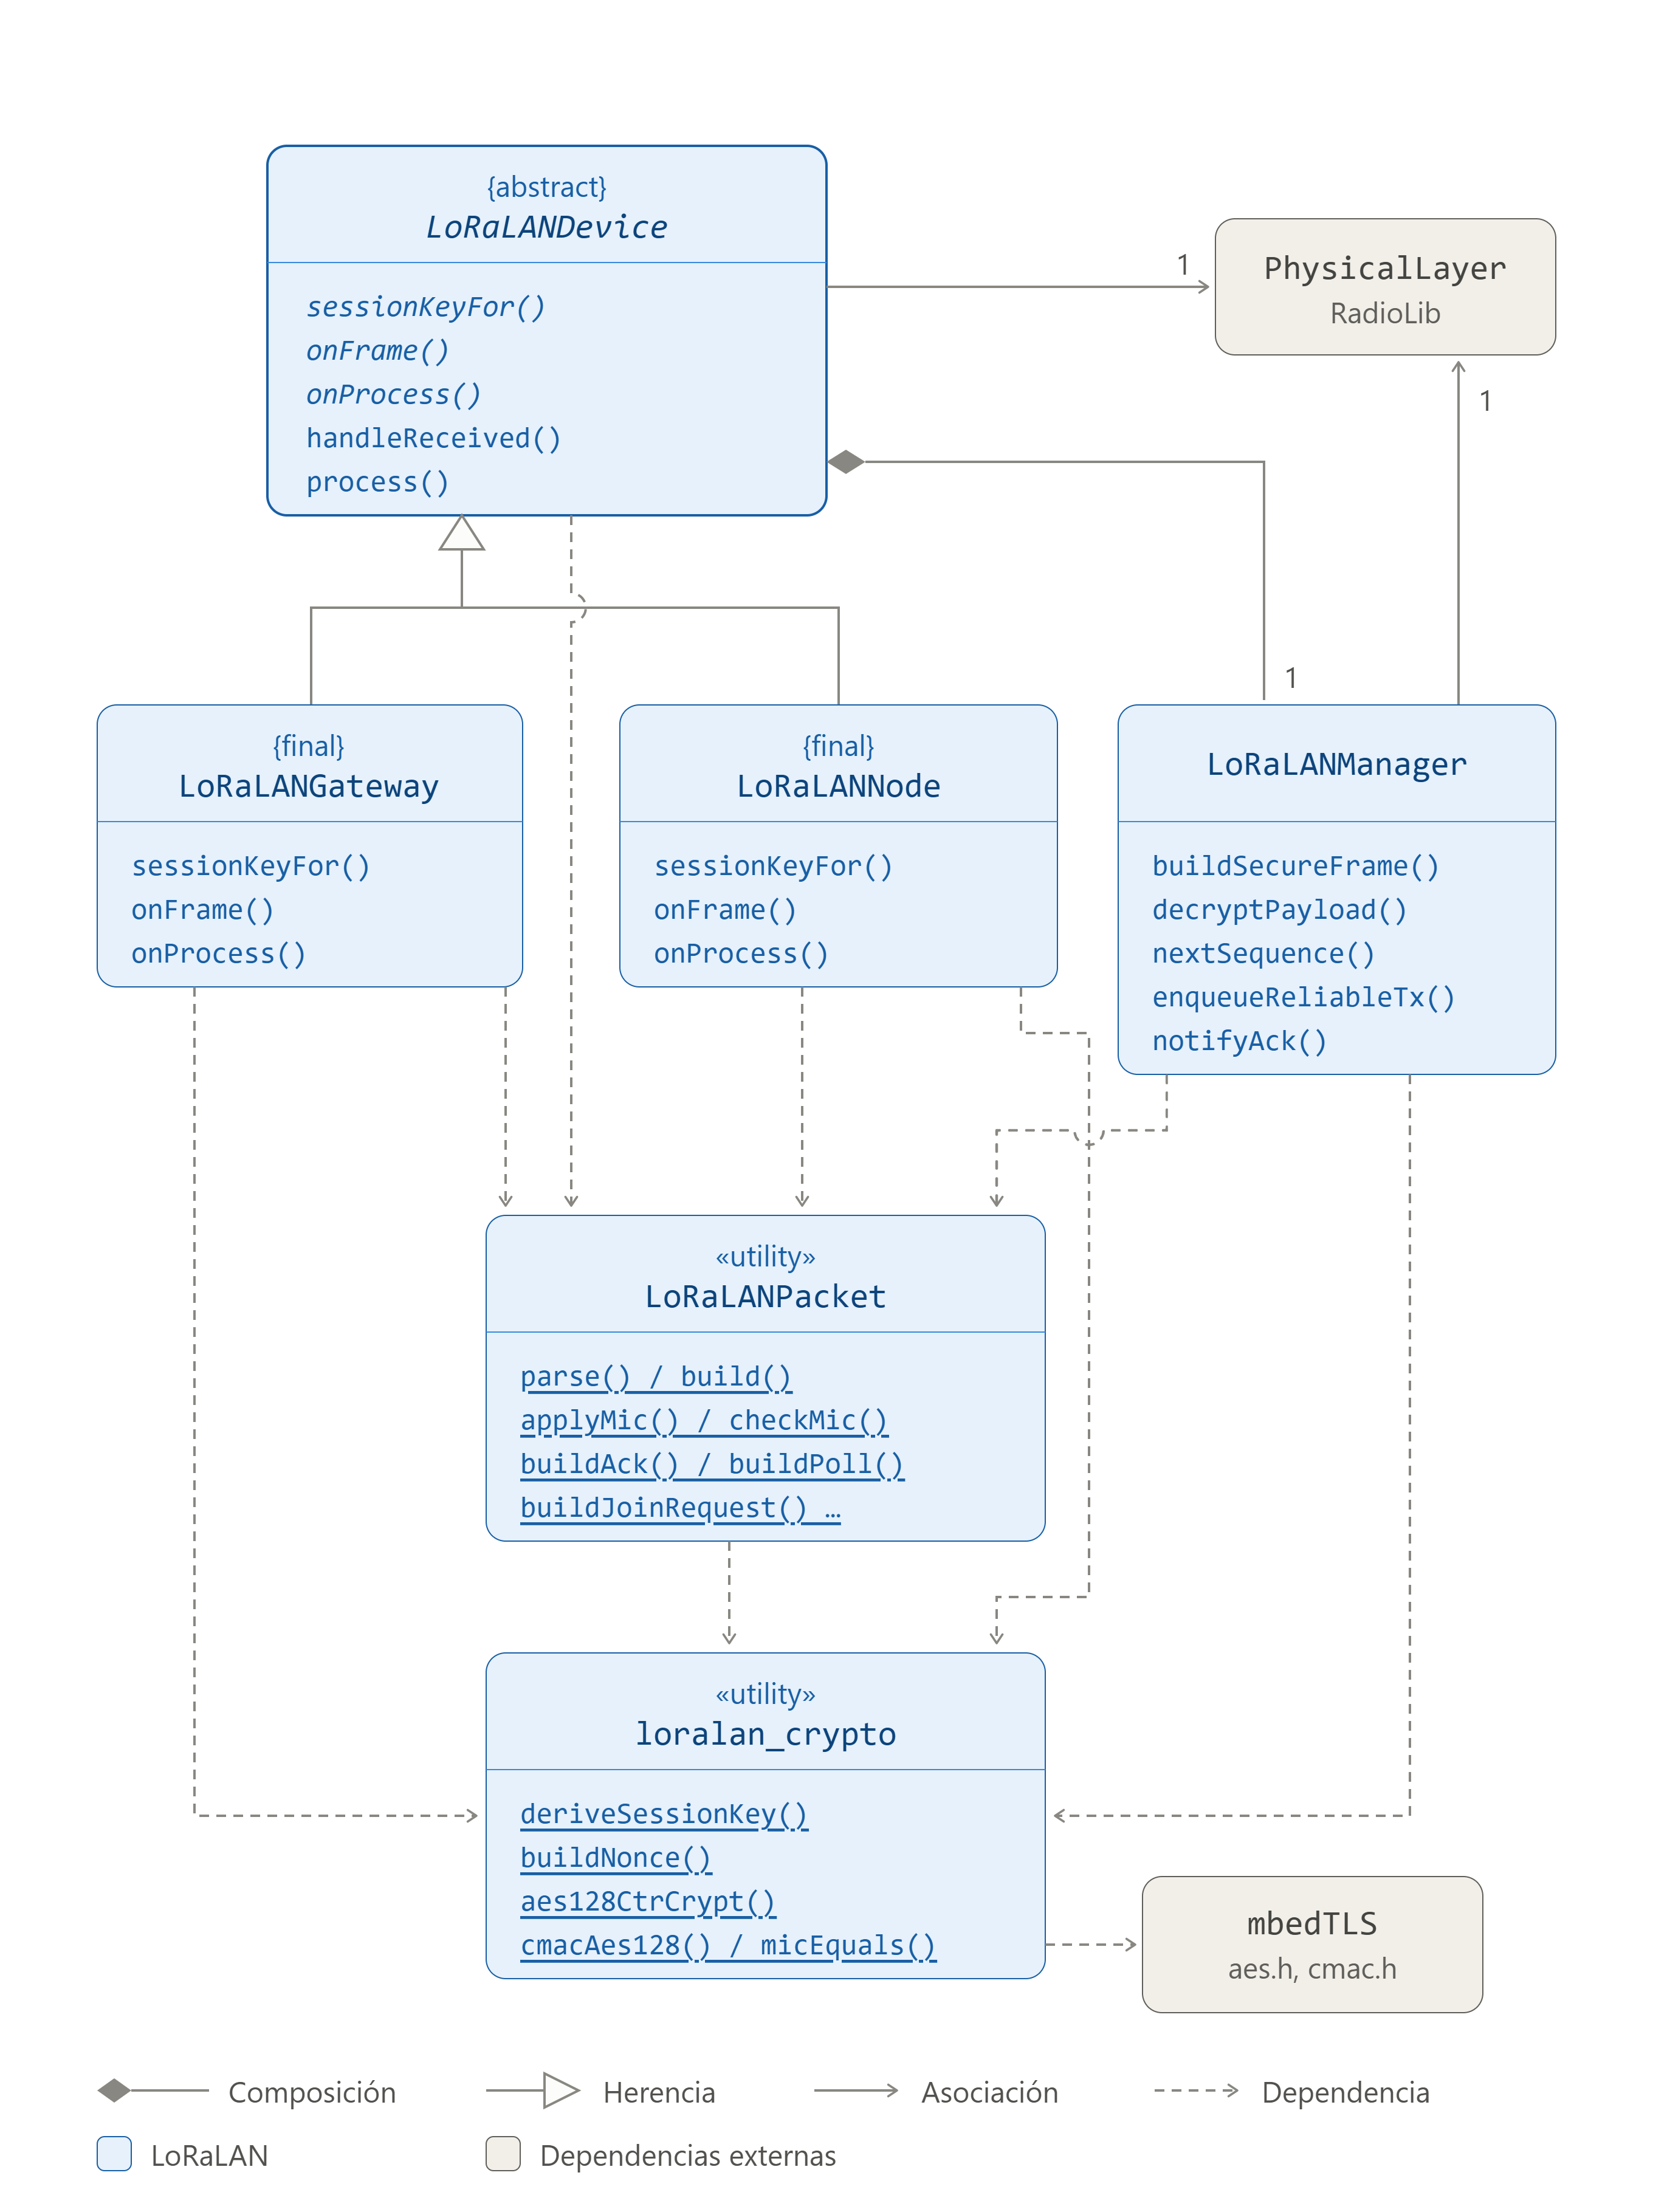
\includegraphics[width=0.95\textwidth]{imagenes/loralan_diagrama_clases_v6.png}
\caption{\label{fig:uml-loralan} Diagrama de módulos UML de la librería LoRaLAN.}
\end{figure}

La lógica de recepción de paquetes se concentra en el módulo base, que comprueba la estructura del paquete, el identificador de red y verifica el MIC antes de entregarlo al rol correspondiente, de forma que una trama sin autenticar no llega a descifrarse ni modifica el estado del dispositivo. En la transmisión, los paquetes que no esperan confirmación se envían directamente, mientras que los que sí la esperan quedan a cargo de \texttt{LoRaLANManager}, que gestiona los plazos y las retransmisiones y que admite un único envío fiable en curso, decisión que simplifica el código a costa de limitar el rendimiento de cada dispositivo.

La librería accede a la radio únicamente a través de \texttt{PhysicalLayer}, la clase base de RadioLib. Por último, su código no reserva memoria dinámica por sí mismo, con la salvedad de la que pueda emplear internamente mbedTLS, ya que todas las estructuras tienen un tamaño fijo y residen dentro de los propios objetos, de manera que la tabla de nodos que emplea el gateway, con 32 entradas de 108~bytes en la compilación para PC, ocupa unos 3,4~kB y en ella se realizan búsquedas lineales, debido a su reducido tamaño.

\section{Interfaz de programación}\label{sec:api}

La interfaz se ha diseñado de modo que la puesta en marcha de un dispositivo sea lo más sencilla posible. Para ello, se crea, en primer lugar, un objeto sobre una radio de RadioLib, se rellena una estructura de configuración, se registran las funciones de retrollamada\footnote{Las funciones de retrollamada o \textit{callbacks} son aquellas que la aplicación define y registra en la librería para que sea esta quien las ejecute cuando se produce un determinado suceso, como la llegada de un paquete.} que interesen y, en el bucle principal, se entregan al objeto los paquetes recibidos y se le llama periódicamente. Por ejemplo, en el Listado~\ref{lst:nodo} se muestra un nodo completo, que se asocia por sí solo y que, a partir de ese momento, envía eventos y responde a los sondeos.


\begin{lstlisting}[language=C++,basicstyle=\ttfamily\footnotesize,frame=single,breaklines=true,breakatwhitespace=true,caption={Ejemplo de implementación de un nodo LoRaLAN.},label={lst:nodo},captionpos=b]
// Transceptor LoRa.
SX1276 radio = new Module(PIN_CS, PIN_DIO0, PIN_RST, RADIOLIB_NC);
LoRaLANNode node(radio);     // nodo LoRaLAN sobre esa radio

// Llamada al recibir una orden valida del gateway
void onCommand(const LoRaLANFrame& frame,
               const uint8_t* payload, uint8_t payloadLen) {
  // orden del gateway, ya descifrada
}
// Llamada al cerrarse un evento push (entregado o no)
void onPushAck(bool delivered,
               const uint8_t* ackPayload, uint8_t ackLen) {
  // desenlace del evento y respuesta de la aplicacion
}

void setup() {
  // 869.525 MHz, BW 125 kHz, SF7, CR 4/5, sync 0x12,
  // 14 dBm, preambulo de 8 simbolos
  int st = radio.begin(869.525, 125.0, 7, 5, 0x12, 14, 8);
  if (st != RADIOLIB_ERR_NONE)
    while (true) {}          // radio no disponible

  // Parametros de red y credenciales del nodo
  LoRaLANNode::Config cfg;
  cfg.netId  = 0x42;         // identificador de la red
  cfg.nodeId = 0x10;         // preferida; 0 = cualquiera
  memcpy(cfg.hwId, MAC, LORALAN_HWID_SIZE);  // id fisico
  cfg.appKey = APP_KEY;      // clave de 16 bytes
  node.begin(cfg);

  // Registro de callbacks de la aplicacion
  node.setOnCommand(onCommand);
  node.setOnPushAck(onPushAck);
  radio.startReceive();      // radio en escucha continua
}

void loop() {
  // 1) Recepcion: se entrega cada trama a la libreria
  if (radio.checkIrq(RADIOLIB_IRQ_RX_DONE) == 1) {
    uint8_t buffer[LORALAN_HEADER_SIZE + LORALAN_MAX_PAYLOAD
                   + LORALAN_MIC_SIZE];  // trama maxima
    size_t len = radio.getPacketLength();
    if (len <= sizeof(buffer) &&
        radio.readData(buffer, len) == RADIOLIB_ERR_NONE)
      node.handleReceived(buffer, len);
    radio.startReceive();    // volver a escuchar
  }

  // 2) Temporizadores, reintentos y envios pendientes
  node.process();

  // 3) Encolado de eventos de la aplicacion
  if (hasEvent && node.queuePushEvent(data, dataLen))
    hasEvent = false;        // la libreria ya tiene su copia
}
\end{lstlisting}


El gateway sigue el mismo patrón, como se observa en el Código~\ref{lst:gateway}, que muestra únicamente la configuración y las operaciones propias del gateway, omitiéndose la inicialización de la radio y la recepción de tramas, que se realizan igual que en el Código~\ref{lst:nodo}. En él se activa la confirmación diferida para que la aplicación responda a cada evento cuando dispone del resultado, que viaja dentro del propio ACK.

\begin{lstlisting}[language=C++,basicstyle=\ttfamily\footnotesize,frame=single,caption={Ejemplo de uso de la librería desde un gateway con confirmación diferida.},label={lst:gateway},captionpos=b]
LoRaLANGateway gateway(radio);

void onPushEvent(const LoRaLANFrame& frame,
                 const uint8_t* payload, uint8_t payloadLen) {
  // se anota (frame.header.srcId, frame.header.seq) y se consulta al servidor
}

void setup() {
  // radio.begin(...) y startReceive() igual que en el nodo
  LoRaLANGateway::Config cfg;
  cfg.netId           = 0x42;
  cfg.gatewayId       = 0x00;
  cfg.appKey          = APP_KEY;
  cfg.pollIntervalMs  = 5000;        // cumple la sub-banda del 10 %
  cfg.deferredPushAck = true;
  gateway.begin(cfg);
  gateway.setOnPushEvent(onPushEvent);
}

void loop() {
  // recepcion igual que en el nodo, con gateway.handleReceived(...)
  gateway.process();                 // POLL, TIME_SYNC y reintentos de CMD
}

// Cuando llega el resultado del servidor para (nodeId, seq):
void onResultado(uint8_t nodeId, uint16_t seq, uint8_t code) {
  gateway.ackPush(nodeId, seq, &code, 1);   // code 0 = OK; otro = NACK
}

// Orden a un nodo; false si ya hay otra 
// en curso o el nodo no esta asociado:
bool enviarOrden(uint8_t nodeId, const uint8_t* cmd, uint8_t len) {
  return gateway.sendCommand(nodeId, cmd, len);
}
\end{lstlisting}


Las operaciones comunes a los dos roles son las siguientes:

\begin{itemize}
\item \textbf{\texttt{begin(config)}}: Aplica la estructura de configuración y reinicia el estado de asociación, lo que en el gateway supone vaciar la tabla de nodos, sin transmitir nada, ya que el nodo inicia la asociación desde \texttt{process}.

\item \textbf{\texttt{handleReceived(buffer, len)}}: Entrega al protocolo un paquete de \texttt{len} bytes recibido por la radio y devuelve \texttt{false} si es inválido, si pertenece a otra red, si no se dispone de clave para su origen, si no supera la verificación del MIC o si se rechaza.

\item \textbf{\texttt{process()}}: Atiende los plazos, las retransmisiones y las tareas periódicas, por lo que debe llamarse continuamente desde el bucle principal.
\end{itemize}

Por su parte, las operaciones principales del nodo son las que se enumeran a continuación:

\begin{itemize}
\item \textbf{\texttt{queuePushEvent(payload, payloadLen, ackRequired, fallbackToPoll)}}: Encola un evento, que se transmite desde \texttt{process} tras escuchar el canal. El parámetro \texttt{ackRequired}, activo por defecto, solicita confirmación, mientras que \texttt{fallbackToPoll}, inactivo por defecto, rescata la carga para el siguiente sondeo si se agotan los intentos, sustituyendo a la que estuviera encolada para ese sondeo. Devuelve \texttt{false} si el nodo no está asociado, si la carga supera los 64~bytes o si ya hay un evento encolado.
\item \textbf{\texttt{queuePollPayload(payload, payloadLen, ackRequired)}}: Prepara la carga de la siguiente respuesta a un sondeo, sustituyendo a la que estuviera encolada. Con \texttt{ackRequired}, activo por defecto, la carga se conserva hasta recibir el ACK. Devuelve \texttt{false} si el nodo no está asociado o si la carga supera los 64~bytes.

\item \textbf{\texttt{requestJoin()}}: Reactiva la asociación automática, que se realiza desde \texttt{process}.

\item \textbf{\texttt{leave()}}: Solicita la baja mediante una trama con confirmación, desactiva la asociación automática y borra la clave de sesión al recibir el ACK o al agotarse los intentos. 
\item \textbf{\texttt{isJoined()}}: Indica si el nodo está asociado.
\item \textbf{\texttt{setOnCommand(cb)}}: Registra la función que recibe las órdenes del gateway ya descifradas.
\item \textbf{\texttt{setOnPushAck(cb)}}: Registra la función que recibe el desenlace de cada evento con confirmación, con los parámetros \texttt{delivered}, que indica si llegó el ACK, y \texttt{ackPayload} y \texttt{ackLen}, que contienen la respuesta de la aplicación. No se invoca si la sesión se pierde antes de conocerse el desenlace.
\item \textbf{\texttt{setOnPollRequest(cb)}}: Registra la función que genera la respuesta a un sondeo cuando no hay ninguna carga encolada.
\item \textbf{\texttt{setOnJoinAccepted(cb)}}: Registra la función a la que se avisa cuando se acepta la asociación.
\end{itemize}

En cuanto al gateway, sus operaciones principales son las siguientes:

\begin{itemize}
\item \textbf{\texttt{sendCommand(nodeId, payload, payloadLen)}}: Envía a \texttt{nodeId} una orden cifrada, con confirmación y reintentos. Devuelve \texttt{false} si el nodo no está asociado, si la carga supera los 64~bytes o si hay otro envío fiable en curso.

\item \textbf{\texttt{ackPush(nodeId, seq, payload, payloadLen)}}: Envía la confirmación del evento \texttt{seq} del nodo \texttt{nodeId}, con una respuesta de aplicación opcional. Devuelve \texttt{false} si ese evento ya no está pendiente.

\item \textbf{\texttt{nodeCount()}}: Devuelve el número de nodos asociados y activos.

\item \textbf{\texttt{isAlive(nodeId, maxAgeMs)}}: Indica si el nodo está asociado y si se ha recibido de él un evento, una respuesta a un sondeo o una solicitud de asociación en los últimos \texttt{maxAgeMs} milisegundos.

\item \textbf{\texttt{nodeHwId(nodeId, out)}}: Copia en \texttt{out} el identificador de fábrica del nodo y devuelve \texttt{false} si este no figura en la tabla.

\item \textbf{\texttt{setOnPushEvent(cb)}, \texttt{setOnPollResponse(cb)}}: Registran las funciones que reciben, ya descifrados, los eventos y las respuestas a los sondeos de los nodos, teniendo en cuenta que estas últimas pueden llegar vacías.

\item \textbf{\texttt{setOnNodeJoined(cb)}, \texttt{setOnNodeLeft(cb)}, \texttt{setOnNodeInactive(cb)}}: Registran las funciones a las que se avisa, con la dirección del nodo, cuando este se asocia, se da de baja o deja de contestar a los sondeos.
\end{itemize}

Los parámetros de temporización son configurables y disponen de los valores por defecto que se recogen en la Tabla~\ref{tab:temporizacion}.

\begin{table}[H]
\centering
\caption{\label{tab:temporizacion} Parámetros de configurables y valores por defecto.}
\begin{tabular}{|l|l|p{6.6cm}|}
\hline
\textbf{Parámetro} & \textbf{Valor} & \textbf{Significado} \\
\hline
\texttt{appAckTimeoutMs} & 1200~ms & Espera de la confirmación tras cada transmisión. \\
\hline
\texttt{appMaxRetries} & 3 & Transmisiones máximas totales: la inicial y dos retransmisiones. \\
\hline
\texttt{joinRetryMs} & 5000~ms & Intervalo entre solicitudes de asociación, sin máximo de intentos. \\
\hline
\texttt{timeSyncIntervalMs} & 30000~ms & Intervalo entre difusiones de la hora. \\
\hline
\texttt{pollIntervalMs} & 2000~ms & Intervalo entre sondeos. \\
\hline
\texttt{maxMissedPolls} & 3 & Sondeos sin respuesta para declarar inactivo un nodo. \\
\hline
\texttt{silenceTimeoutMs} & 0 & Detección de silencio del nodo, desactivada por defecto. \\
\hline
\end{tabular}
\end{table}

Los sondeos cada 2000~ms suponen por sí solos, en SF7, un 2,06~\% de ciclo de trabajo, sin contar el resto de las tramas del gateway. La detección de silencio se deja desactivada porque su plazo depende del número de nodos y del periodo de sondeo de cada instalación.

Debe tenerse en cuenta que un valor de retorno \texttt{true} en las operaciones de envío significa únicamente que la petición se ha aceptado, y no que la trama haya llegado a su destino. Asimismo, las cargas que se entregan a estas operaciones se copian o se transmiten durante la propia llamada, por lo que la aplicación no necesita conservarlas después.

Los \textit{callbacks} se ejecutan de forma síncrona dentro de la llamada a \texttt{handleReceived} o a \texttt{process} que los origina, y los punteros que reciben solo son válidos mientras dura la función, de modo que su contenido debe copiarse si se necesita más adelante o desde otro hilo. Puesto que una operación lenta en ellos retrasa la recepción, los plazos, las retransmisiones y las tareas periódicas, el gateway del prototipo no realiza en sus \textit{callbacks} ninguna operación de red y se limita a encolar los datos para que los atiendan otros hilos, tal como se describe más adelante.

En cuanto a las confirmaciones, se distinguen dos tipos:

\begin{itemize}
\item \textbf{Confirmación automática}: Se envía al retornar el \textit{callback}, para toda trama aceptada que la solicite y vaya dirigida al dispositivo, mientras que el emisor espera 1200~ms por defecto, más un retardo aleatorio de hasta 600~ms, antes de retransmitir.

\item \textbf{Confirmación diferida}: Se aplica a los eventos con confirmación cuando \texttt{deferredPushAck} está activo, de modo que el ACK no se envía al retornar el \textit{callback}, sino cuando la aplicación llama a \texttt{ackPush}. Mientras no lo haga, las retransmisiones del nodo quedan sin respuesta, por lo que la aplicación debe contestar antes de que este agote sus intentos y, a ser posible, antes de su primera retransmisión, lo que en el prototipo se garantiza con la cadena de plazos del apartado~\ref{sec:gwlinux}.
\end{itemize}

Por último, la librería no inicializa la radio ni detecta la llegada de los paquetes, sino que es la aplicación la que configura el transceptor, decide si atiende la recepción por interrupción o por consulta y entrega cada trama al protocolo, aunque la transmisión y la exploración del canal sí se realizan desde la librería. Gracias a ello, esta se integra tanto en el bucle de un programa de Arduino como en la tarea de FreeRTOS del nodo o en el hilo de radio del gateway, si bien no incorpora mecanismos de exclusión mutua, por lo que todas las llamadas a un mismo objeto deben realizarse desde un único hilo. Debe considerarse, además, que la transmisión y la exploración del canal son bloqueantes, de modo que las llamadas que las realizan se prolongan al menos durante el tiempo en el aire de la trama, lo que ha de tenerse en cuenta si ese hilo asume otras tareas.

\section{Implementación del nodo en la aplicación registro de asistencia}\label{sec:nodo-app}

En este apartado se describe cómo se ha implementado el firmware del nodo en el sistema de fichaje que se desarrolla en el trabajo. El nodo conserva el hardware del sistema de partida, formado por un ESP32, un lector NFC PN532, los sensores BME280, BH1750 y LD2410, una pantalla OLED, dos relés, tres LED y un zumbador, y añade un transceptor SX1276 que comparte el bus SPI con el lector. Puesto que el nodo debe atender a la vez el protocolo de radio y todos estos periféricos, el mayor riesgo es que una operación lenta, como una lectura por I$^2$C o el refresco de la pantalla, interfiera en la comunicación. Por eso, se aprovechan los dos núcleos del ESP32, de manera que todo lo relativo a la radio se concentra en una tarea fijada al núcleo~0, mientras que la gestión de la aplicación se ejecuta en el núcleo~1, como se muestra en la Figura~\ref{fig:nodo-tareas}.

\begin{figure}[H]
\centering
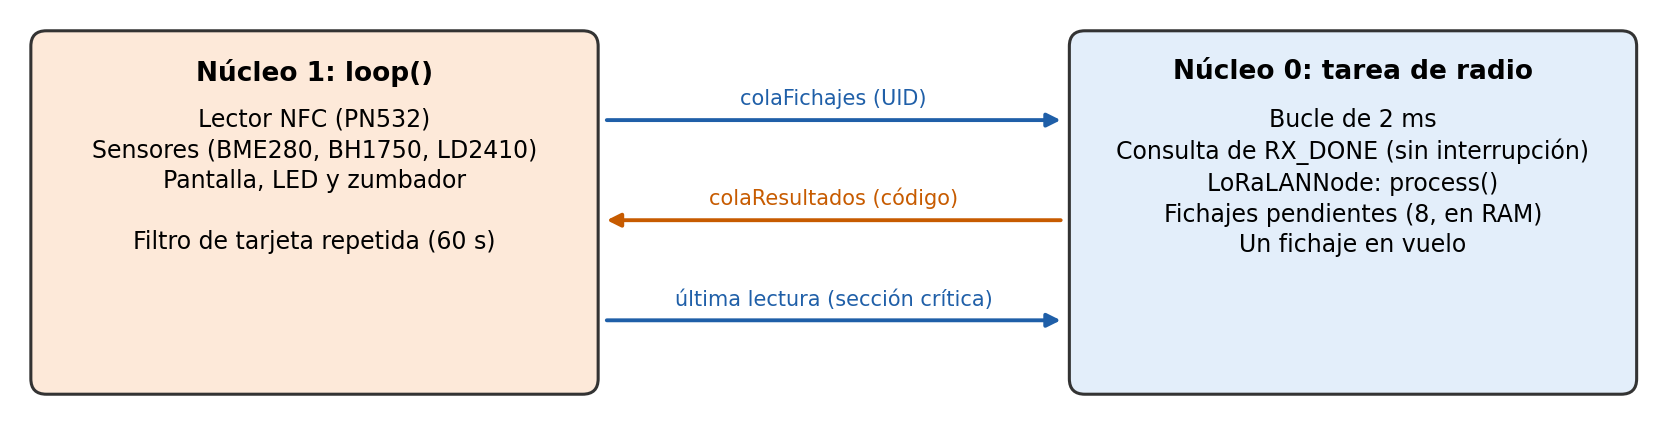
\includegraphics[width=0.88\textwidth]{imagenes/nodo_tareas.png}
\caption{\label{fig:nodo-tareas} Reparto del firmware del nodo entre los dos núcleos del ESP32.}
\end{figure}

Ambos núcleos se comunican sin bloquearse mediante dos colas del sistema operativo, una para los fichajes leídos y otra para sus resultados, y una copia de la última lectura de los sensores protegida frente al acceso simultáneo. La tarea de radio repite cada 2~ms el mismo ciclo, en el que comprueba si ha llegado una trama, la entrega a \texttt{handleReceived} y llama a \texttt{process}. Para detectar paquetes se consulta el registro de estado del transceptor en lugar de emplear su interrupción, debido a que la detección de actividad de canal señala el fin de la exploración (\textit{CadDone}) por la misma línea DIO0 y provocaría falsas recepciones.

Sobre esta estructura, cada función de la aplicación utiliza el mecanismo de la biblioteca que mejor se adapta a ella. Un fichaje se envía mediante \texttt{queuePushEvent} y su resultado llega en la respuesta de aplicación del ACK, que se obtiene a través de \texttt{setOnPushAck} y que distingue si el fichaje se ha registrado, si se ha rechazado de forma definitiva o si debe reintentarse. Las lecturas de los sensores y el estado de los relés se generan bajo demanda en la función registrada con \texttt{setOnPollRequest} y no solicitan confirmación, puesto que una lectura perdida se sustituye por la del sondeo siguiente. Por último, las órdenes del gateway llegan a través de \texttt{setOnCommand} y actúan sobre los relés o programan un reinicio, que se retrasa un segundo para que antes pueda enviarse el ACK de la propia orden.

Dado que la biblioteca admite un único evento encolado, la cola de fichajes pendientes es responsabilidad de la aplicación, que conserva hasta ocho fichajes en memoria RAM y mantiene uno solo en curso, de modo que el ACK recibido corresponde siempre al primero de la cola. Si no llega, el fichaje pasa al final de la cola y no vuelve a enviarse hasta pasados 30~s. Además, como la biblioteca descarta sin notificarlo el evento en curso cuando el nodo pierde la asociación, la aplicación deja de esperar su desenlace si detecta esa pérdida
o si transcurren 20~s sin conocerlo, y el primero de la cola se envía de nuevo en cuanto el nodo vuelve a estar asociado.

Al arrancar por primera vez, el nodo solicita una dirección dinámica y guarda en memoria no volátil la que le asigna el gateway. En los arranques siguientes solicita esa misma dirección y conserva su identidad en el servidor y, con ella, su aula. Por último, se activa la detección de silencio con un plazo equivalente a tres vueltas de sondeo, el máximo admitido, y el intervalo de sondeo de 5~s del gateway, de modo que, si el gateway se reinicia y deja de reconocer al nodo, este repite la asociación hasta que el gateway responde.

\section{Gateway sobre Linux en Raspberry Pi}\label{sec:gwlinux}

Implementar el gateway sobre un microcontrolador presenta una limitación práctica a la hora de comunicarse con el servidor, debido a que la pila de red y la radio compiten por el mismo procesador. Por este motivo, para el sistema de registro de asistencia, el gateway se ha implementado como un proceso de Linux sobre una Raspberry Pi, con un módulo SX1276 conectado por SPI.

La adaptación sigue el procedimiento descrito anteriormente. Por un lado, una capa implementa las funciones del entorno Arduino sobre las del sistema operativo, empleando un reloj monótono que no salta cuando el sistema ajusta su hora. Por otro lado, se utiliza la adaptación para Raspberry Pi que RadioLib incluye para acceder al SPI y a las líneas de entrada y salida, de modo que la librería LoRaLAN se compila sin modificar.

El proceso reparte su trabajo en los tres hilos que se muestran en la Figura~\ref{fig:gw-hilos}, unidos mediante colas, con el fin de que la radio no espere nunca a una operación de red. Una petición HTTP lenta dentro del \textit{callback} de recepción retrasaría el ACK más allá del plazo del nodo, y de hecho este defecto existía en el primer puente desarrollado para ESP32, que realizaba la petición dentro del \textit{callback} con un plazo de tres segundos, frente a los 1,2~segundos que espera el nodo. A continuación se detallan las responsabilidades de cada hilo.

\begin{figure}[H]
\centering
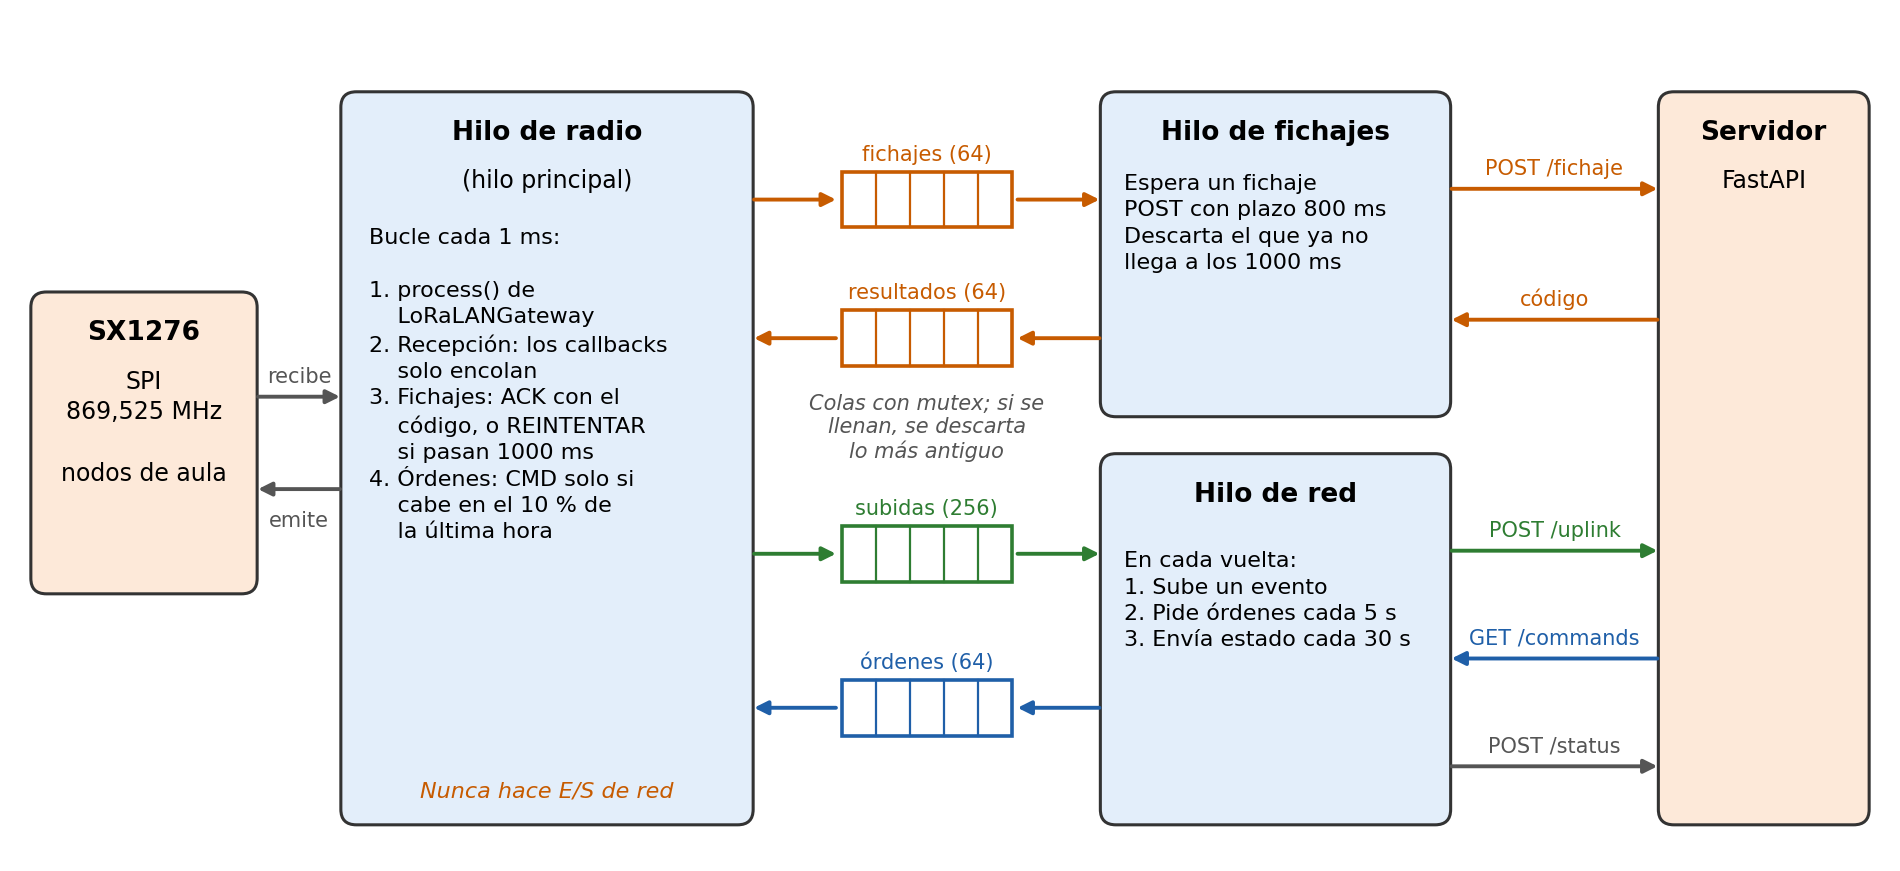
\includegraphics[width=0.88\textwidth]{imagenes/gateway_hilos.png}
\caption{\label{fig:gw-hilos} Hilos del gateway y colas que los unen.}
\end{figure}


\begin{itemize}
\item \textbf{Hilo de radio}: Ejecuta el protocolo y nunca realiza operaciones de red, ya que los \textit{callbacks} de la librería se limitan a encolar.

\item \textbf{Hilo de fichajes}: Consulta al servidor cada fichaje con un plazo de 800~ms y se separa del resto de comunicaciones para que una subida lenta de telemetría no le haga perder ese plazo.

\item \textbf{Hilo de red}: Sube la telemetría y las altas y bajas de nodos, recoge las órdenes del servidor cada 5~segundos y envía un informe de estado cada 30~segundos.
\end{itemize}

Si una cola se llena, se descarta el elemento más antiguo y se contabiliza en el informe de estado, puesto que perder una lectura antigua es preferible a detener la radio. La traducción entre el formato binario de la radio y el JSON del servidor reside en un módulo sin entrada ni salida, probado en PC, que convierte en REINTENTAR cualquier respuesta del servidor que no sea un código reconocible.

El gateway incorpora, además, dos piezas para el control del ciclo de trabajo de las que la librería carece:

\begin{itemize}
\item \textbf{Cálculo del tiempo en el aire}: Obtiene el de cualquier trama a partir de su longitud y de los parámetros de radio, según la ecuación del fabricante (ec.~\ref{eq:toa}).

\item \textbf{Contador de ciclo de trabajo}: Registra en una ventana deslizante el tiempo en el aire de las transmisiones de la última hora e indica si una nueva cabe en el presupuesto.
\end{itemize}

Con ellas, el gateway realiza dos comprobaciones. En primer lugar, al arrancar calcula qué fracción del ciclo de trabajo consumirá el sondeo, que es el mayor consumidor de tiempo en el aire, y, si excede el límite de la sub-banda, \textbf{termina con un error} en lugar de emitir de más en silencio. En segundo lugar, durante la ejecución comprueba que cada orden cabe en el presupuesto antes de transmitirla y, en caso contrario, la retiene hasta que quepa. Como el ciclo de trabajo de la sub-banda es, como máximo, del 10\,\%, no se espera que se dé esta circunstancia salvo en despliegues con mucho tráfico de eventos.

\section{Skill para desarrollo de aplicaciones para LoRaLAN mediante IA generativa}\label{sec:skill}

La revolución de la inteligencia artificial generativa y el desarrollo agéntico han cambiado por completo la forma en la que se desarrolla software~\cite{willison2026agentic}. Por ello, se ha considerado conveniente que la biblioteca incluya una \textit{skill} destinada a apoyar el desarrollo de aplicaciones que empleen LoRaLAN.

Una \textit{skill} es un paquete autocontenido de instrucciones, scripts y
recursos, organizado en un directorio cuyo elemento central es un fichero
\texttt{SKILL.md}, que un agente de IA descubre y carga dinámicamente para
especializarse en una tarea concreta. Su carga es progresiva: el agente solo
conoce inicialmente el nombre y la descripción de cada \textit{skill}, lee las
instrucciones completas cuando la considera relevante y accede a los ficheros
adicionales únicamente si la tarea lo requiere, lo que permite ampliar sus
capacidades sin saturar la ventana de contexto \cite{anthropic2025skills}.

La \textit{skill} se distribuye con la biblioteca en el fichero skills/loralan/SKILL.md, que el IDE de Arduino ignora durante la compilación. Para utilizarla, basta con copiarla al directorio de \textit{skills} de la herramienta de desarrollo agéntico que se desee.

Su contenido reúne las características principales del protocolo, los patrones de uso de la biblioteca, sus restricciones y las instrucciones para ejecutar las pruebas con el simulador. De este modo, proporciona a los agentes de programación el contexto necesario para utilizar LoRaLAN correctamente, evitando que propongan métodos inexistentes o soluciones incompatibles con su diseño.

Esta guía no sustituye a la documentación de la biblioteca ni garantiza la corrección del código generado, que sigue requiriendo revisión y pruebas. Asimismo, debe mantenerse actualizada cuando cambie la interfaz de programación.


\section{Síntesis del capítulo}

En este capítulo se ha abordado la implementación de LoRaLAN como una biblioteca modular escrita en C++, separando la lógica del protocolo de los detalles específicos de cada plataforma. Para ello, se ha definido una arquitectura organizada en seis módulos y una API que facilita su integración en aplicaciones. Asimismo, se ha adaptado la biblioteca para su compilación y ejecución en distintos entornos, desde microcontroladores ESP32 hasta sistemas Linux y un simulador para ordenador.

A partir de esta implementación se han desarrollado un firmware de referencia para los nodos ESP32 y una aplicación de pasarela para Raspberry Pi. Esta última incorpora una arquitectura concurrente que desacopla las comunicaciones LoRa de las operaciones de red y mecanismos de control del ciclo de trabajo. Finalmente, se ha creado una \textit{skill} que proporciona a los agentes de programación información contextual sobre el protocolo y facilita su utilización durante el desarrollo de aplicaciones.
\chapter{Validación del protocolo LoRaLAN}\label{chap:6}

Tras diseñar e implementar LoRaLAN, es necesario validar su funcionamiento más allá de comprobar que el caso de uso funcione sobre hardware. Para ello, se desarrollan un simulador específico y un plan de pruebas a partir de los requisitos del protocolo. El capítulo describe ambos elementos, presenta los resultados disponibles y analiza las limitaciones de la validación.

Dado que la simulación permite reproducir de forma controlada situaciones difíciles de provocar sobre hardware real, constituye el principal método de verificación del protocolo.  


\section{Diseño del simulador}\label{sec:disenosim}

El simulador que se describe en este apartado, denominado \texttt{sim\_LoRaLAN}, se ha diseñado de forma que cumpla cuatro condiciones:

\begin{itemize}
\item \textbf{Aislamiento}: cada caso se ejecuta en un entorno nuevo y no depende de lo que dejaron los casos anteriores.
\item \textbf{Inyección de fallos}: cada caso provoca un fallo concreto, sin depender de que la pérdida aleatoria lo produzca.
\item \textbf{Observabilidad}: las comprobaciones se hacen sobre una traza consultable, no sobre la salida por consola.
\item \textbf{Determinismo}: con un reloj virtual y una semilla, la misma semilla siempre da la misma traza.
\end{itemize}

La librería se compila directamente a partir de sus ficheros fuente, sin modificarlos. Sin embargo, LoRaLAN depende de tres bibliotecas externas pensadas para ejecutarse en un microcontrolador, no en un ordenador. Para resolverlo, se sustituye cada una por una versión simplificada que ofrece las mismas funciones con los mismos nombres, de modo que la librería las utiliza sin notar la diferencia. Las bibliotecas que se sustituyen son:

\begin{itemize}
\item \textbf{Arduino}: Proporciona el reloj, los números aleatorios y la salida por consola. En el simulador, \texttt{millis()} es un reloj virtual que solo avanza cuando el simulador lo indica, así que minutos de protocolo se ejecutan en una fracción de segundo. \texttt{random()} usa un generador propio, de modo que una misma semilla da los mismos valores en cualquier ordenador.

\item \textbf{RadioLib}: Controla el chip LoRa SX1276. Se sustituye por una radio ficticia conectada al canal simulado que devuelve los mismos códigos de estado que el chip real, de los que depende la librería.

\item \textbf{mbedTLS}: Aporta el cifrado AES y la autenticación CMAC. Se sustituye por funciones simples que dan un resultado distinto según la clave. No ofrecen seguridad real y solo sirven para comprobar que cada trama usa la clave correcta.
\end{itemize}

Para comprobar los casos de prueba, el simulador necesita saber por qué se rechaza cada paquete. Sin embargo, la librería no lo indica. Cuando se recibe un paquete, solo se informa si se acepta o rechaza.

Por eso, el simulador deduce el motivo por su cuenta. En la mayoría de los casos (formato incorrecto, otra red, otro destinatario o clave equivocada) lo consigue con funciones que la propia librería ofrece. La única excepción es el fallo de autenticación: la librería no lo comunica por ninguna vía salvo un mensaje de aviso que escribe en la consola. Como el simulador usa su propia versión de la consola, puede leer ese mensaje y reconocer el fallo.

El simulador está escrito en C++ y se compila con CMake. Su arquitectura separa la ejecución de los casos, la simulación del medio y la evaluación de los resultados. El núcleo crea el gateway y los nodos, gestiona el avance del tiempo y modela el canal. Una traza registra los acontecimientos y permite comprobar las propiedades de cada caso y calcular su veredicto. Los casos de prueba definen las situaciones que se provocan y las condiciones que deben cumplirse.

Se contempla que el tiempo avance en pasos fijos de 1~ms. En cada paso, el gateway y los nodos ejecutan \texttt{process()}. Después, el canal entrega los paquetes que han terminado, se anotan los cambios de estado y avanza el reloj. Se ha elegido un paso fijo porque la librería consulta \texttt{millis()} en cada llamada a \texttt{process()}, igual que en el bucle de una placa.

Las cifras de rendimiento dependen de cómo se simule el canal, por lo que se declaran sus propiedades en la Tabla~\ref{tab:modelo-canal}. El tiempo en el aire se calcula según la longitud, con la misma fórmula que emplea el gateway de la Raspberry Pi (ecuación~\ref{eq:toa}).

\begin{table}[H]
\centering
\caption{\label{tab:modelo-canal} Hipótesis realizadas para modelar el canal.}
\begin{tabular}{|p{2.8cm}|p{11.3cm}|}
\hline
\textbf{Aspecto} & \textbf{Modelo} \\
\hline
Tiempo en el aire & Fórmula de Semtech según la longitud, redondeada al milisegundo superior. Puede sustituirse por un valor medido. \\
\hline
Escucha del canal & Instantánea. Una trama no se detecta hasta $W$~ms después de comenzar (ventana ciega) y, a partir de ahí, se detecta durante toda su duración. Salvo que un caso indique otra cosa, $W = 0$. \\
\hline
Pérdida & Independiente por receptor y por enlace, sin ráfagas. Una trama perdida ocupa el aire igual que las demás. \\
\hline
Colisión & Cualquier solapamiento entre radios distintas destruye ambas tramas para todos los receptores. \\
\hline
Semidúplex & El emisor no ejecuta \texttt{process()} hasta terminar su emisión. \\
\hline
Reloj & Único y sin deriva. \\
\hline
Radio & La emisión y la escucha nunca devuelven error. La recepción invoca directamente \texttt{handleReceived()}. \\
\hline
\end{tabular}
\end{table}

La ventana ciega, representada por $W$, es el intervalo desde el inicio de una transmisión hasta que los demás dispositivos pueden detectarla. Su valor permite estudiar situaciones en las que dos nodos comienzan a transmitir sin detectarse mutuamente. Por ello, los resultados que dependen de este parámetro se interpretan como un análisis de sensibilidad.

La aleatoriedad se controla mediante una semilla que determina las esperas del protocolo, las pérdidas y los instantes de llegada de los mensajes PUSH. Las pérdidas utilizan un generador independiente del empleado por la librería, evitando que modificar su probabilidad altere también las esperas del protocolo. Así, una misma configuración puede reproducirse y compararse bajo distintas condiciones.

Cada caso declara los fallos que provoca mediante estímulos como el descarte selectivo de tramas, identificado por tipo, sentido y número de aparición, la ocupación del canal, el corte de enlace o la presencia de un atacante.

La traza registra el instante, el dispositivo, el tipo de trama, su secuencia y, cuando procede, el motivo de descarte. Las propiedades se comprueban mediante consultas sobre estos registros, que también pueden exportarse a CSV para su análisis.

Finalmente, los veredictos se asignan individualmente a cada propiedad, en lugar de agruparse por caso, ya que una misma ejecución puede satisfacer unos requisitos e incumplir otros. Se distinguen tres resultados: Superado, Fallido y No concluyente.

\section{Plan de pruebas}\label{sec:plan-pruebas}

La validación combina dos tipos de pruebas. Por un lado, las pruebas funcionales verifican que el protocolo funciona tal y como se ha descrito en la fase de diseño. Por otro lado, se realizan pruebas experimentales que miden el comportamiento de la red ante ciertas situaciones.

Ambos tipos se complementan, ya que un caso funcional demuestra que un mecanismo actúa o falla en una situación, mientras que un experimento indica con qué frecuencia se da esa situación y qué coste tiene. Así, el caso U5 comprueba que un evento perdido se repite y se entrega una sola vez, y EXP1 mide qué parte de los eventos llega cuando las pérdidas son aleatorias.

\subsection{Pruebas funcionales}\label{sec:plan-funcional}

Cada prueba funcional recorre una misma cadena: requisito, propiedad, resultado esperado, estímulo, ejecución, veredicto y resolución. El resultado esperado se obtiene del requisito previamente definido, ya que, si se escribiera después, se daría por bueno lo que el código ya hace. 

Por ello, si un caso falla no se modifica lo esperado para que se supere, sino que el fallo se registra y, después, se decide si se corrige el código, si se revisa el requisito de forma justificada o si se documenta la limitación. Dado que cada caso provoca un fallo concreto, una sola ejecución basta para obtener su veredicto, por lo que la batería se ejecuta con una semilla fija y se repite con otras 30 únicamente para comprobar que los veredictos no dependen del azar.

Los identificadores de estas pruebas siguen la convención que se muestra en la Tabla~\ref{tab:nomenclatura}, en la que la letra indica la parte del protocolo que se prueba. Las 76~pruebas de protocolo se distribuyen entre las familias J, L, P, U, D, C, T, S y A. Los números no expresan importancia y presentan huecos porque el catálogo de partida contenía demasiadas pruebas funcionales; se han seleccionado 87 según su prioridad y el plazo disponible.

\begin{table}[H]
\centering
\caption{\label{tab:nomenclatura} Identificadores de las pruebas.}
\begin{tabular}{|c|p{2.9cm}|p{7.0cm}|c|}
\hline
\textbf{Prefijo} & \textbf{Familia} & \textbf{Qué se comprueba} & \textbf{Casos} \\
\hline
SIM & Simulador & El propio simulador & 5 \\
\hline
F & Formato & Construcción y lectura de paquetes & 6 \\
\hline
J & JOIN & Incorporación a la red & 13 \\
\hline
L & LEAVE & Baja de la red & 9 \\
\hline
P & POLL & Ventana de sondeo & 12 \\
\hline
U & PUSH (\textit{o uplink}) & Eventos que el nodo emite por iniciativa propia & 20 \\
\hline
D & ACK diferido & Respuesta de la aplicación dentro de la confirmación & 5 \\
\hline
C & CMD & Órdenes del gateway a un nodo & 6 \\
\hline
T & TIME\_SYNC & Difusión de la hora & 3 \\
\hline
S & Silencio & Reacción a la ausencia o al reinicio del gateway & 3 \\
\hline
A & Ataque & Tramas falsas, alteradas, repetidas o malformadas & 5 \\
\hline
\end{tabular}
\end{table}

En el Anexo \ref{anexo_A} se relacionan las pruebas de formato y las 76~pruebas de protocolo. Salvo que la situación indique otra cosa, el escenario está formado por un nodo asociado y un canal limpio, sin sondeo automático y con una ventana ciega nula. El símbolo $^{\dagger}$ señala los casos en los que, antes de ejecutarlos, se preveía que el código no cumpliera lo esperado.

\subsection{Pruebas experimentales}\label{sec:experimentos}

Los casos anteriores comprueban si el protocolo reacciona correctamente ante una situación concreta, pero no indican cómo se comporta la red en funcionamiento continuo. Por ello, los experimentos no emiten un veredicto, sino que miden cómo cambia el comportamiento de la red al variar ciertos factores.

Salvo que se indique otra cosa, se emplea la configuración del despliegue: SF7, sondeo cada 5~s, sincronización cada 30~s y respuestas al sondeo de 10~bytes. Los fichajes son eventos de 6~bytes con confirmación inmediata y, cuando se simula tráfico continuo, llegan a la red según un proceso de Poisson, es decir, en instantes aleatorios e independientes entre sí. Cada experimento persigue un objetivo concreto:

\begin{itemize}
    \item \textbf{VAL}: Se ejecuta para comprobar la validez del simulador ante un resultado teórico conocido. Un nodo emite un evento cada 6~s y se aplican distintos niveles de pérdida (0, 10, 20, 35 y 50\,\%) únicamente en la subida.

    \item \textbf{EXP1}: Se estudia el efecto de las pérdidas en ambos sentidos. Se analiza tanto la entrega y latencia de eventos aislados como la detección de inactividad mediante cuatro nodos que responden al sondeo.

    \item \textbf{EXP4}: Se evalúa la contención entre eventos sin sondeo. La ventana ciega $W$ permite estudiar la sensibilidad de las colisiones a este parámetro, cuyo valor real no se ha medido, por lo que los resultados no predicen directamente el comportamiento en un despliegue.

    \item \textbf{EXP5}: Se repite el escenario de EXP4 con sondeo para aislar el efecto del POLL. También se estudia la influencia de su intervalo, las pérdidas de comunicación y el número de nodos.
    
\end{itemize}

Cada configuración se repite con 30~semillas, salvo los barridos por ventana de sondeo y con 254~nodos, que emplean entre 3 y 10 porque son más lentos o tienen poca componente aleatoria. Estas repeticiones son necesarias porque el resultado depende del azar: permiten observar sucesos poco frecuentes, que podrían no aparecer en una sola ejecución, y estimar la incertidumbre de cada cifra comparando las réplicas entre sí.

Del catálogo inicial de experimentos propuestos, se han mantenido los experimentos más relevantes, lo que explica los huecos en la numeración.


\subsection{Trazabilidad de los requisitos}\label{sec:trazabilidad}

En la Tabla~\ref{tab:trazabilidad} se relaciona cada requisito con las pruebas que lo verifican. Algunos requisitos no pueden comprobarse en un simulador, por lo que se indica también el método externo correspondiente.

{\small
\begin{longtable}{|c|p{4.4cm}|p{8.2cm}|}
\caption{\label{tab:trazabilidad} Correspondencia entre requisitos y pruebas.}\\
\hline
\textbf{Req.} & \textbf{Enunciado abreviado} & \textbf{Verificación prevista} \\
\hline
\endfirsthead
\hline
\textbf{Req.} & \textbf{Enunciado abreviado} & \textbf{Verificación prevista} \\
\hline
\endhead
PRO-1 & Comunicación entre nodos y gateway & J5, P10 \\
\hline
PRO-2 & Telemetría e inactivos & P1--P3, P5, P7, P8, P11; EXP1, EXP3 \\
\hline
PRO-3 & Eventos asíncronos & J4, U1--U3, U10--U16, D1--D4, D6; EXP4, EXP5; escucha real en hardware \\
\hline
PRO-4 & Comunicación descendente & C1, C3--C5 \\
\hline
PRO-5 & Confirmación de entrega & L5, P4, P6, P9, P14, U4--U9, U17, U20, U22, C2, C3; VAL, EXP1, EXP7 \\
\hline
PRO-6 & Incorporación y salida & J1--J3, J6--J8, J10, J15, L1--L4, L6, L7, L9; vectores publicados \\
\hline
PRO-7 & Sincronización temporal & T1, T2, T-PER \\
\hline
PRO-8 & Seguridad & F1, F3--F5, J12, J13, L10, C1, C7, A1--A5; vectores publicados y captura en hardware. Sin prueba válida de la solidez del cifrado en el simulador \\
\hline
PRO-9 & Recuperación ante la pérdida del gateway & T2, U17, S1, S2, S4; EXP3, EXP7 \\
\hline
RNF-1 & Eficiencia & U1; EXP1, EXP5; medida en hardware \\
\hline
RNF-2 & Cumplimiento normativo & Ciclo de trabajo (apartado~\ref{sec:dutycycle}); EXP3, EXP5; tiempo en el aire medido en hardware \\
\hline
RNF-3 & Recursos y capacidad & F2, F6, J9, U19; búsqueda de memoria dinámica en los fuentes; lista de componentes \\
\hline
RNF-4 & Portabilidad e integración & Compilación sin cambios en ESP32, Raspberry Pi y PC; ejemplo mínimo de nodo y de gateway \\
\hline
RNF-5 & Verificabilidad & SIM1--SIM5, VAL \\
\hline
\end{longtable}
}


\section{Resultados de rendimiento y limitaciones}\label{sec:resultados}
% Sustituye al apartado «Resultados de la batería» del capítulo 6.
% Cifras: sim_LoRaLAN, commit 1902369, semilla 42 (results/casos.csv) y semillas 1 a 30.

\subsection{Resultados de la batería}\label{sec:estado-ejecucion}

La batería se ejecutó en el simulador sobre la versión final de la librería y con la semilla fija con la que se obtienen todos los veredictos de este apartado. De los 87~casos, 78 se superan por completo y 9 presentan alguna propiedad Fallida. En total, 141~propiedades se superan, 11 fallan y ninguna queda No concluyente, de modo que todas llegaron a ejercitar el estímulo que declaran. La Tabla~\ref{tab:bateria} resume estos resultados por familia.


\begin{table}[H]
\centering
\caption{\label{tab:bateria} Resultado de la batería por familia.}
\small
\setlength{\tabcolsep}{6pt}
\begin{tabular}{|l|c|c|c|c|}
\hline
\textbf{Familia} & \textbf{Casos} & \textbf{Con fallos} & \textbf{Prop. superadas} & \textbf{Prop. fallidas} \\
\hline
Simulador (SIM) & 5 & 0 & 14 & 0 \\
\hline
Formato (F) & 6 & 0 & 14 & 0 \\
\hline
JOIN (J) & 13 & 1 & 22 & 2 \\
\hline
LEAVE (L) & 9 & 2 & 14 & 2 \\
\hline
POLL (P) & 12 & 1 & 15 & 1 \\
\hline
PUSH (U) & 20 & 3 & 31 & 3 \\
\hline
ACK diferido (D) & 5 & 1 & 5 & 1 \\
\hline
CMD (C) & 6 & 0 & 11 & 0 \\
\hline
TIME\_SYNC (T) & 3 & 0 & 4 & 0 \\
\hline
Silencio (S) & 3 & 0 & 4 & 0 \\
\hline
Seguridad (A) & 5 & 1 & 7 & 2 \\
\hline
\textbf{Total} & \textbf{87} & \textbf{9} & \textbf{141} & \textbf{11} \\
\hline
\end{tabular}
\end{table}

Para comprobar el determinismo del simulador, la batería se ejecutó dos veces con la misma semilla, obteniéndose ficheros de resultados y trazas idénticos byte a byte. Asimismo, se repitió con las semillas 1 a 30 para verificar que los veredictos no dependen del azar, y el único que cambió fue el de U16, que se supera en 15 de las 30~ejecuciones, lo que resulta coherente con que su resultado dependa de las esperas aleatorias de los nodos que colisionan.

En la Tabla~\ref{tab:fallidas} se relacionan los nueve casos que mantienen alguna propiedad Fallida, junto con el tratamiento que se ha decidido para cada uno. Ninguno de ellos se ha corregido, de modo que todos se mantienen como limitaciones declaradas de la versión final, bien porque su corrección exigiría modificar el protocolo, bien porque sus efectos son poco frecuentes o recuperables o bien porque dependen de magnitudes físicas que solo pueden medirse en hardware.

La primera ejecución de la batería, sobre la versión anterior a la validación, identificó 17~casos con alguna propiedad Fallida, de los que se corrigieron ocho tras analizar sus causas. En concreto, U22, U20, C3 y C7 se resolvieron con el control de secuencia implementado, U4 limitando a ocho las escuchas de un evento con el canal ocupado y J5 con una espera aleatoria en los reintentos y en la asociación, mientras que L6 se corrigió impidiendo que el nodo confirme órdenes durante la baja y A3 descartando los ACK cuyo destino no es el receptor. La batería completa se repitió después de cada corrección, hasta obtener los nueve casos fallidos de la Tabla~\ref{tab:fallidas}.

{\small
\begin{longtable}{|c|p{8.2cm}|c|p{3.4cm}|}
\caption{\label{tab:fallidas} Casos con alguna propiedad Fallida en la versión final.}\\
\hline
\textbf{Caso} & \textbf{Comportamiento observado} & \textbf{Req.} & \textbf{Tratamiento} \\
\hline
\endfirsthead
\hline
\textbf{Caso} & \textbf{Comportamiento observado} & \textbf{Req.} & \textbf{Tratamiento} \\
\hline
\endhead
J13 & Un JOIN antiguo capturado y repetido se acepta, puesto que el gateway solo recuerda el último DevNonce, y la sesión del nodo legítimo deja de funcionar. & PRO-8 & Limitación: corregirlo cambia el protocolo de asociación. \\
\hline
A4 & El contador de 16~bits da la vuelta sin renovar la clave, de modo que el mismo texto se cifra igual dos veces, y una orden capturada vuelve a ejecutarse pasada media escala del contador del gateway, unas 39~h con sondeo cada 5~s y sincronización cada 30~s. & PRO-8 & Limitación: exige renovar la clave dentro de la sesión. \\
\hline
L4 & Con un envío pendiente de confirmación, \texttt{leave()} devuelve \texttt{false}, pero el nodo se da de baja localmente sin avisar al gateway. & PRO-6 & Limitación: situación poco frecuente. \\
\hline
L5 & Al darse de baja con un evento en cola, el evento se descarta sin avisar a la aplicación con \texttt{delivered=false}. & PRO-5 & Limitación: situación poco frecuente. \\
\hline
P6 & Una segunda carga para el sondeo sobrescribe a la pendiente en lugar de rechazarse, por lo que la primera no llega a entregarse. & PRO-5 & Limitación: el nodo dispone de una sola carga pendiente. \\
\hline
U9 & El rescate de un evento no entregado sobrescribe la carga que ya esperaba al sondeo, que no llega a entregarse. & PRO-5 & Limitación: misma causa que P6. \\
\hline
U15 & El reintento de un evento se emite sin escuchar el canal, de modo que no detecta que está ocupado. & PRO-3 & Limitación: escuchar podría hacer perder el ACK, como en el defecto~4, y debe probarse en hardware. \\
\hline
U16 & Con $W = 2$~ms, cuatro nodos que emiten a la vez entregan los cuatro eventos en 15 de 30~semillas, con una media de 3,3~eventos entregados. & PRO-3 & Limitación: depende de una ventana ciega aún sin medir. \\
\hline
D6 & El ACK diferido del gateway se destruye al coincidir con la respuesta del nodo a un POLL, aunque el evento se entrega al retransmitirse. & PRO-3 & Limitación: se recupera con la retransmisión. \\
\hline
\end{longtable}
}

Los nueve casos que mantienen fallos estaban señalados con $^{\dagger}$ en la Tabla~\ref{tab:catalogo}, es decir, su comportamiento problemático se había anticipado.

\subsection{Resultados de las pruebas experimentales}\label{sec:resultados-exp}

A continuación se evalúan los experimentos de la estrés sobre la red. Se ejecutaron con 30~semillas por configuración. Las tasas se acompañan de su intervalo de confianza del 95\,\% sobre el total de eventos y las latencias se expresan como la media, entre réplicas, de la mediana y de los percentiles de cada una.

\subsubsection{Validación del simulador (VAL)}

Primero, conviene comprobar que el simulador reproduce un caso de solución conocida. Se consideran tres intentos y una pérdida independiente $p$ únicamente en la subida, de modo que el ACK, que viaja en bajada, llega siempre. En estas condiciones, un evento solo deja de entregarse si se pierden los tres intentos, lo que ocurre con probabilidad $p^{3}$, por lo que la tasa de entrega es $E = 1 - p^{3}$. Por su parte, se denomina TX al número medio de transmisiones que necesita un evento para llegar al gateway, que se obtiene ponderando por su probabilidad las tres formas de llegar, en el primer, el segundo o el tercer intento:

\begin{equation}
E = 1 - p^{3}, \qquad \mathrm{TX} = \frac{(1-p) + 2p(1-p) + 3p^{2}(1-p)}{1 - p^{3}}
\end{equation}

Como se observa en la Tabla~\ref{tab:teoria}, los resultados simulados concuerdan con los valores teóricos. La mayor diferencia en la tasa de entrega se produce con un 35\,\% de pérdida y es de 0,4 puntos porcentuales, dentro de la variabilidad esperable para una simulación de 6000 eventos. Asimismo, los valores de TX coinciden hasta la segunda cifra decimal. Este contraste valida la implementación de la lógica de reintentos y del modelo de pérdida del simulador, aunque no permite extraer conclusiones sobre el comportamiento del canal real, que requiere medidas sobre hardware.

\begin{table}[H]
\centering
\caption{\label{tab:teoria} Valores teóricos y simulados con tres intentos y pérdida solo en la subida (VAL, 6000~eventos por nivel). TX es el número medio de transmisiones por evento entregado.}
\small
\setlength{\tabcolsep}{4pt}
\begin{tabular}{|c|c|c|c|c|}
\hline
\textbf{Pérdida} & \textbf{Entrega teórica} & \textbf{Entrega simulada (IC 95\,\%)} & \textbf{TX teórica} & \textbf{TX simulada} \\
\hline
0\,\%  & 100,0\,\% & 100,0\,\% (\ldots) & 1,00 & 1,00 \\
\hline
10\,\% & 99,9\,\%  & 99,9\,\% (\ldots)  & 1,11 & 1,11 \\
\hline
20\,\% & 99,2\,\%  & 99,2\,\% (\ldots)  & 1,23 & 1,23 \\
\hline
35\,\% & 95,7\,\%  & 95,3\,\% (\ldots)  & 1,40 & 1,40 \\
\hline
50\,\% & 87,5\,\%  & 87,3\,\% (\ldots)  & 1,57 & 1,57 \\
\hline
\end{tabular}
\end{table}

\subsubsection{Latencia y entrega frente a la pérdida (EXP1)}\label{sec:latencia}

El experimento EXP1 evalúa la entrega fiable ante pérdidas en ambos sentidos, midiendo el tiempo desde que el nodo encola un evento hasta que el gateway lo recibe. Los niveles de pérdida más altos se plantean como escenarios de estrés, no como condiciones habituales de despliegue. Los resultados se recogen en la Tabla~\ref{tab:latencia}.



\begin{table}[H]
\centering
\caption{\label{tab:latencia} Latencia y fiabilidad de un evento frente a la pérdida (EXP1, 6000~eventos por nivel).}
\footnotesize
\setlength{\tabcolsep}{3pt}
\begin{tabular}{|c|c|c|c|c|c|c|}
\hline
\textbf{Pérdida} & \textbf{Entrega (IC 95\,\%)} & \textbf{Confirmados} & \textbf{Mediana} & \textbf{p95} & \textbf{p99} & \textbf{TX/evento} \\
\hline
0\,\%  & 100,0\,\% (99,9--100,0) & 100,0\,\% & 52~ms & 52~ms & 52~ms & 1,00 \\
\hline
10\,\% & 99,9\,\% (99,8--100,0) & 99,2\,\% & 52~ms & 1553~ms & 2066~ms & 1,23 \\
\hline
20\,\% & 99,5\,\% (99,2--99,6) & 95,2\,\% & 52~ms & 1876~ms & 3186~ms & 1,50 \\
\hline
35\,\% & 95,4\,\% (94,8--95,9) & 80,6\,\% & 52~ms & 2993~ms & 3381~ms & 1,92 \\
\hline
50\,\% & 87,7\,\% (86,8--88,5) & 58,0\,\% & 52~ms & 3116~ms & 3427~ms & 2,31 \\
\hline
\end{tabular}
\end{table}

Las retransmisiones mantienen la entrega por encima del 87\,\% incluso con la mitad de las tramas perdidas. El coste es un mayor número de transmisiones (hasta 2,31 por evento) y una latencia en p95--p99 de varios segundos, debida a los plazos de confirmación y a las esperas entre reintentos. La mediana, en cambio, se mantiene en 52~ms, el tiempo en el aire de un \texttt{PUSH\_EVENT}. La confirmación se degrada antes que la entrega: con un 20\,\% de pérdida, el 4,2\,\% de los eventos llegó al gateway sin que el nodo recibiera el ACK.

En conjunto, el mecanismo es robusto en entrega y su coste se concentra en latencia y consumo de canal, no en pérdida de datos. Que el nodo reciba «no entregado» no implica que el evento se haya perdido: puede haber llegado al gateway sin que llegara su ACK.

\subsubsection{Contención y colisiones (EXP4 y EXP5)}\label{sec:contencion}

Los experimentos EXP4 y EXP5 aplican el mismo tráfico de eventos sin sondeo y con sondeo cada 5~s, respectivamente, de modo que su diferencia es el coste que introduce el POLL. Ambos varían además la ventana ciega $W$ y el número de nodos. Puesto que el valor real de $W$ se desconoce, los resultados de la Tabla~\ref{tab:contencion} no predicen el comportamiento en despliegue, sino la tolerancia del protocolo ante distintos parámetros.

\begin{table}[H]
\centering
\caption{\label{tab:contencion} Colisiones, entrega y latencia con 60~fichajes por minuto en redes de 8 y 32~nodos (EXP4 sin sondeo y EXP5 con sondeo cada 5~s).}
\small
\setlength{\tabcolsep}{4pt}
\begin{tabular}{|c|c|c|c|c|c|c|c|}
\hline
\multirow{2}{*}{\textbf{Sondeo}} & \multirow{2}{*}{\textbf{$W$ (ms)}} & \multicolumn{2}{c|}{\textbf{Destruidas}} & \multicolumn{2}{c|}{\textbf{Entrega}} & \multicolumn{2}{c|}{\textbf{p99}} \\
\cline{3-8}
 & & \textbf{8 nodos} & \textbf{32 nodos} & \textbf{8 nodos} & \textbf{32 nodos} & \textbf{8 nodos} & \textbf{32 nodos} \\
\hline
No & 0 & 0,18\,\% & 0,20\,\% & 99,99\,\% & 99,99\,\% & 271~ms  & 290~ms \\
\hline
No & 2 & 0,80\,\% & 0,88\,\% & 99,95\,\% & 99,95\,\% & 452~ms  & 397~ms \\
\hline
No & 5 & 2,22\,\% & 2,46\,\% & 99,88\,\% & 99,84\,\% & 1608~ms & 1439~ms \\
\hline
Sí & 0 & 1,59\,\% & 1,66\,\% & 99,97\,\% & 99,96\,\% & 1467~ms & 1453~ms \\
\hline
Sí & 2 & 2,18\,\% & 2,27\,\% & 99,92\,\% & 99,92\,\% & 1569~ms & 1563~ms \\
\hline
\end{tabular}
\end{table}

Como se observa en la Tabla~\ref{tab:contencion}, las retransmisiones recuperan casi todas las emisiones destruidas y la entrega se mantiene prácticamente completa. El aumento de 8 a 32~nodos apenas modifica los resultados cuando se mantiene constante el tráfico total. Por otra parte, las colisiones aumentan con la ventana ciega (del 0,18 al 2,46\,\% sin sondeo) y el sondeo introduce colisiones adicionales, ya que el gateway transmite sus ACK y POLL sin escuchar el canal. Esta decisión simplifica su funcionamiento y garantiza la puntualidad de las respuestas, pero incrementa la latencia: aunque la mayoría de los eventos llega en el primer intento, los afectados por colisiones suelen necesitar retransmisiones, lo que eleva los percentiles superiores por encima del segundo.



\subsubsection{Tiempo en el aire y ciclo de trabajo}\label{sec:dutycycle}

Como complemento, se realizan estimaciones del ciclo de trabajo del gateway. El tiempo en el aire de cada trama se obtiene mediante la ecuación~\ref{eq:toa} con SF7, 125~kHz, CR~4/5, preámbulo de 8~símbolos, cabecera explícita y CRC. Con estos parámetros, las tramas van desde unos 41~ms para las que no llevan carga, como el \texttt{POLL} o el \texttt{ACK}, hasta unos 133~ms para la trama máxima. Un \texttt{PUSH\_EVENT} con un registro de asistencia ocupa 51,5~ms, que el simulador redondea a 52~ms.

El ciclo de trabajo de cada dispositivo depende solo de unos pocos parámetros del protocolo:
\begin{equation}
\label{eq:duty}
DC_{\text{gw}} = \frac{T_{\text{POLL}} + a\,T_{\text{ACK}}}{T_{\text{poll}}} + \frac{T_{\text{SYNC}}}{T_{\text{sync}}},
\qquad
DC_{\text{nodo}} = \frac{T_{\text{RESP}}}{N\,T_{\text{poll}}}
\end{equation}
donde $T_{\text{poll}}$ es el intervalo entre dos \texttt{POLL} consecutivos, $T_{\text{sync}}$ el intervalo de sincronización, $N$ el número de nodos y $a$ la fracción de respuestas que requieren confirmación.

Con un sondeo cada 5~s y una sincronización cada 30~s, el gateway ocupa el canal un 0,98\,\% del tiempo (0,82\,\% por los \texttt{POLL} y 0,15\,\% por los \texttt{TIME\_SYNC}). Este valor sube al 1,80\,\% en el caso extremo en que todas las respuestas requieren confirmación, y llega al 5,09\,\% medido en EXP5 con 60~eventos por minuto, en todos los casos por debajo del límite. Un nodo, en una red de un solo nodo, ocupa un 1,13\,\%, y este valor se divide entre $N$ a medida que la red crece, porque sus turnos se espacian. Por tanto, el protocolo escala bien en este aspecto: el consumo del gateway depende únicamente de $T_{\text{poll}}$ y no del número de nodos. Aun así, la librería comprueba este valor al arrancar y se niega a iniciar el gateway si el sondeo configurado excede el límite; con el intervalo por defecto de 2~s, los \texttt{POLL} suponen un 2,06\,\%, todavía lejos de él.

Este margen depende, sobre todo, del factor de ensanchamiento. Con SF12 las tramas son unas 28~veces más largas (un \texttt{POLL} pasa de 41,2 a 1155~ms), por lo que el intervalo entre \texttt{POLL} debería superar los 11,6~s para que el gateway siga por debajo del ciclo de trabajo máximo, como se recoge en la Tabla~\ref{tab:duty}.

\begin{table}[H]
\centering
\caption{\label{tab:duty} Intervalo mínimo entre \texttt{POLL} según el factor de ensanchamiento (125~kHz, CR~4/5).}
\begin{tabular}{|c|c|c|}
\hline
\textbf{SF} & \textbf{ToA del \texttt{POLL}} & \textbf{$T_{\text{poll}}$ mínimo} \\
\hline
7  & 41,2~ms   & 0,41~s \\ \hline
8  & 82,4~ms   & 0,82~s \\ \hline
9  & 144,4~ms  & 1,44~s \\ \hline
10 & 288,8~ms  & 2,89~s \\ \hline
11 & 577,5~ms  & 5,78~s \\ \hline
12 & 1155,1~ms & 11,6~s \\ \hline
\end{tabular}
\end{table}

\subsection{Limitaciones detectadas}\label{sec:limitaciones-val}

Los resultados de este capítulo deben interpretarse teniendo en cuenta tres tipos de límites: los del propio simulador, las limitaciones que conserva el protocolo en su versión final y el alcance, todavía reducido, de la validación sobre placas reales.

En primer lugar, el canal virtual no está calibrado frente a medidas reales: no modela ruido, desvanecimiento ni obstáculos que degraden la señal, por lo que las pérdidas y colisiones son una abstracción del comportamiento físico. Además, el simulador no aplica los mecanismos criptográficos del diseño, sino un MIC ficticio. Por último, los resultados esperados los redacta quien diseñó el protocolo y solo se ejecuta una selección del catálogo de pruebas, de modo que superar la batería no garantiza la ausencia de defectos y sería necesario ampliar su cobertura.

En segundo lugar, la versión final del protocolo conserva las siguientes limitaciones:

\begin{itemize}

\item \textbf{Fallos descubiertos}: los nueve casos de la Tabla~\ref{tab:fallidas} impiden afirmar que se cumplan por completo los requisitos PRO-3, PRO-5, PRO-6 y PRO-8. Entre ellos destacan dos debilidades de seguridad distintas. Por un lado, como el gateway solo recuerda el último DevNonce, un JOIN antiguo capturado puede repetirse y aceptarse, lo que deja sin servicio la sesión del nodo legítimo. Por otro, el contador de 16~bits da la vuelta sin que se renueve la clave, por lo que una orden capturada vuelve a ser válida pasada media escala del contador.

\item \textbf{Gateway sin escucha previa}: el gateway emite sus POLL y sus ACK sin comprobar si el canal está ocupado. En las condiciones simuladas, en torno a un 1\,\% de los eventos colisiona con un POLL en su primer intento, aunque esta cifra depende del escenario y no puede generalizarse.

\item \textbf{Recuperación lenta tras el reinicio del gateway}: los nodos solo detectan el reinicio por la ausencia de paquetes, de modo que no se reasocian hasta que vence el plazo de silencio, de tres rondas de sondeo sin actividad, y durante ese tiempo se pierde la mayor parte de los eventos. Este plazo tampoco puede reducirse por debajo del tiempo entre dos turnos de un mismo nodo, porque en ese caso los nodos se reasociarían sin motivo.

\item \textbf{Capacidad}: la red admite 32~nodos y, con un POLL cada 5~s, cada nodo recibe su turno cada $5N$~s, es decir, cada 160~s con la tabla completa, lo que limitará la posibilidad de adquirir telemetría dependiendo de la aplicación concreta y de la información a transmitir.
\end{itemize}

Por último, la validación sobre hardware se limita a un escenario de laboratorio con dos placas ESP32 con SX1276 y una tercera como analizador. En él se verificaron la asociación automática, el funcionamiento conjunto del nodo y del gateway sobre Raspberry Pi, la interoperabilidad de la criptografía real y la confirmación con carga útil. Quedan sin medir en placas reales el alcance y el comportamiento con muchos nodos.

\section{Síntesis del capítulo}

En este capítulo se ha validado LoRaLAN mediante un simulador que ejecuta la librería real sin modificarla. Sobre él se han ejecutado 87~casos funcionales, vinculados a los requisitos del Capítulo~\ref{chap:3}, y varios experimentos de rendimiento.

El simulador reprodujo los valores teóricos y la batería detectó fallos reales. Tras las correcciones, se superan todas las propiedades de PRO-1, PRO-2, PRO-4, PRO-7 y PRO-9. Sin pérdidas, la entrega superó el 99,8\,\% con una mediana de 52~ms. Con pérdidas, el protocolo se degradó de forma gradual y se recuperó de todos los cortes. Además, el ciclo de trabajo del gateway queda muy por debajo del 10\,\% y no depende del número de nodos sino de la frecuencia a la que se consulte a los nodos.

Sin embargo, nueve casos siguen fallando, lo que impide afirmar el cumplimiento completo de PRO-3, PRO-5, PRO-6 y PRO-8. Destacan la repetición de JOIN bajo algunas circunstancias y de órdenes antiguas, la ausencia de escucha previa en el gateway, la recuperación lenta tras su reinicio y los falsos inactivos. Como todas las cifras proceden de un simulador sin calibrar y la validación en hardware es todavía limitada, estos resultados no sustituyen en ningún caso a pruebas realizadas sobre hardware.
\chapter{Caso de uso: Sistema de Registro de Asistencia y Monitoreo de Aulas}\label{chap:7}

En este capítulo se pone a prueba LoRaLAN con la aplicación que motivó el trabajo, el sistema de registro de asistencia del profesorado y monitorización de aulas implementado sobre la red Wi-Fi del edificio, que se migra a una red LoRaLAN. A continuación, se describen la arquitectura extremo a extremo, la capa de aplicación diseñada sobre LoRaLAN, encargada de comunicar los nodos con el servidor, y el recorrido de un fichaje. Además se muestra el diseño llevado a cabo para fabricar una PCB para el prototipo y posteriormente se detalla el servidor, la base de datos y, finalmente, se exponen las pruebas realizadas y se expone el diseño y empleo de un monitor de red a partir de un Cardputer M5 con un módulo SX1262.

\section{Sistema de partida y requisitos}

El sistema, desarrollado en el Centro Universitario de Mérida, como ya se ha comentado anteriormente, consta de un dispositivo por aula basado en ESP32, con un lector NFC para la tarjeta del profesor, sensores ambientales y de presencia, dos relés e indicadores. La aplicación se conecta con un servidor desarrollado con FastAPI en Python e implementa persistencia conectándose a una base de datos relacional con MySQL. El servidor decide si los registros de asistencias son válidos verificando la tarjeta con el horario del aula. Además el sistema ofrece paneles web para que los profesores puedan consultar sus horarios lectivos y el recuento de clases impartidas al mes. A los conserjes se les facilita un panel que permite consultar el estado de las aulas y la información relativa a sus sensores. A los administradores se les facilita un panel para administrar los nodos LoRaLAN. El dispositivo y el servidor se comunicaban a través de la red Wi-Fi del edificio, por la que el dispositivo enviaba los fichajes por HTTP y mantenía una conexión WebSocket permanente para la telemetría y las órdenes. 

La especificación de requisitos completa se recoge en el Capítulo~\ref{chap:3}. Los casos de uso que atraviesan la red de radio son fichar, supervisar un aula, accionar un relé y reiniciar un dispositivo.

La correspondencia con las clases de tráfico del apartado~\ref{sec:escenario} es directa, ya que el fichaje es el evento, la telemetría es el tráfico periódico y los relés son las órdenes.

\section{Arquitectura de extremo a extremo}

En la Figura~\ref{fig:arquitectura} se muestra la arquitectura del sistema tras la migración, junto con los tres flujos que la recorren: el fichaje, la monitorización y el control.

\begin{figure}[H]
\centering
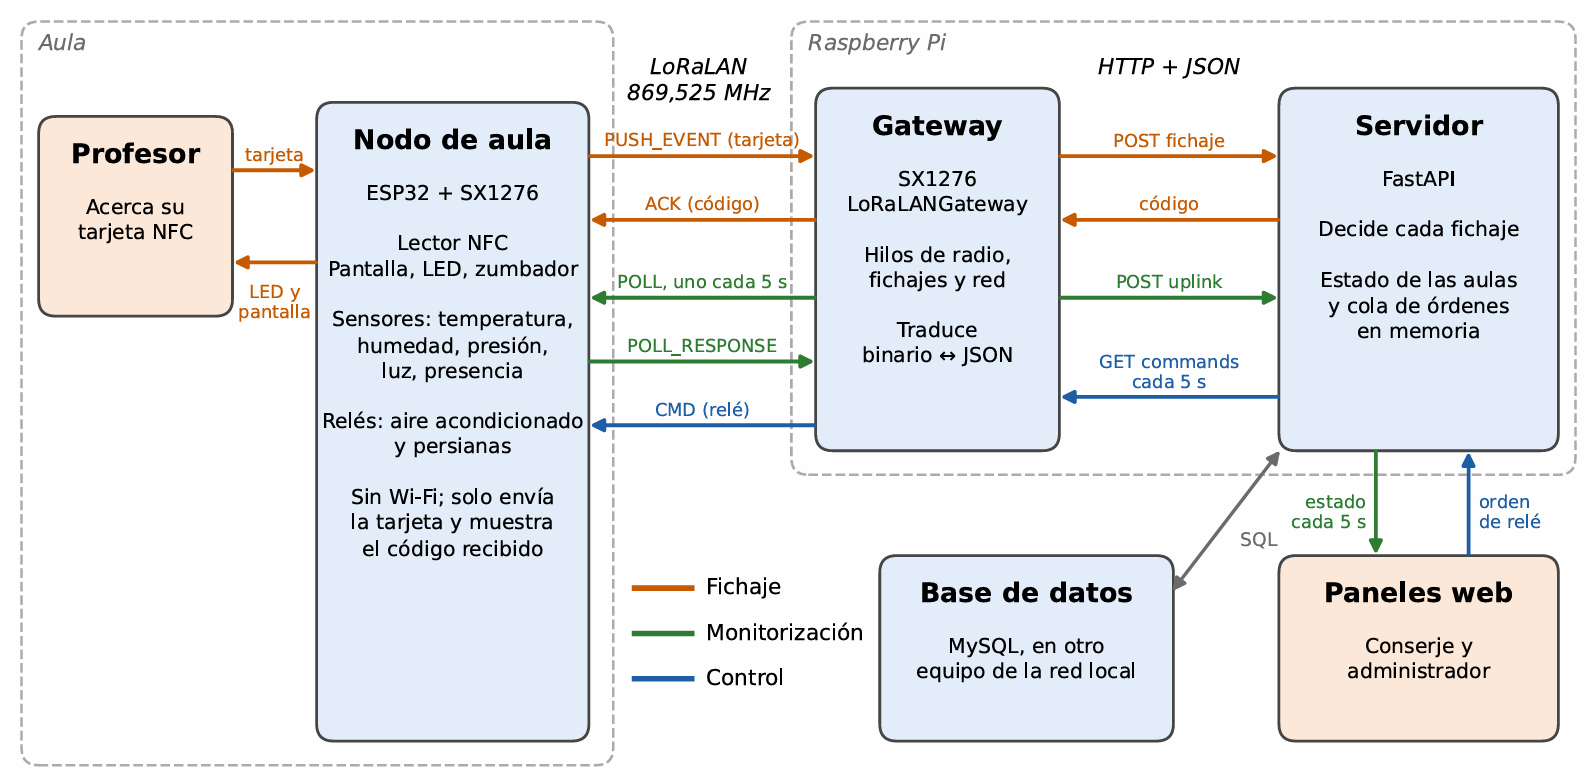
\includegraphics[width=\textwidth]{imagenes/esquema de fichaje.png}
\caption{\label{fig:arquitectura} Arquitectura del sistema de registro de asistencia y monitoreo de nodos sobre LoRaLAN.}
\end{figure}

El nodo de aula se limita a enviar el identificador de la tarjeta leída y la telemetría, y a mostrar el código de resultado recibido. El gateway, ejecutado en una Raspberry Pi, es el único punto de contacto entre las redes de radio e IP y traduce los mensajes binarios de los nodos a peticiones HTTP con cuerpo JSON, y viceversa. El servidor implementa la lógica de negocio y la gestión de la base de datos, pero se comunica exclusivamente con el gateway, mientras que los paneles web consultan periódicamente su estado. En el prototipo, el gateway y el servidor se ejecutan en la misma Raspberry Pi, mientras que la base de datos se puede ejecutar en el mismo equipo o en otra máquina.

La migración elimina todas las conexiones WebSocket y sustituye la comunicación permanente por consultas periódicas del gateway al servidor. Esto se realiza para centralizar el control de las transmisiones en el gateway. De este modo, el servidor registra las órdenes pendientes y el gateway las consulta y transmite cuando considera oportuno o cuando su presupuesto de ciclo de trabajo lo permite.

La lógica de negocio sobre los fichajes sigue correspondiendo al servidor, que conoce la existencia de las tarjetas, los horarios de clase y los profesores asignados a cada asignatura. Esto simplifica el nodo y evita distribuir información de horarios por la red de radio, aunque exige que la respuesta llegue al nodo dentro del plazo de un intercambio. Este requisito motivó la confirmación con carga útil del protocolo (apartado~\ref{sec:ackdiferido}).

\section{Capa de aplicación sobre LoRaLAN}\label{sec:appprotocol}

Dado que LoRaLAN transporta cargas opacas, su significado lo define una capa de aplicación propia que se especifica en un único fichero de cabecera, \texttt{AppProtocol.h}, compartido por el firmware del nodo y el gateway, de modo que ambos extremos compilan la misma definición. El primer byte de cada mensaje identifica su tipo y los valores de varios bytes viajan con el byte más significativo en primer lugar (\textit{big-endian}), como se muestra en la Tabla~\ref{tab:appmsg}. La idea es implementar una capa de aplicación sencilla que sea capaz de transportar la mayor cantidad de información en el menor número de bytes posible.

\begin{table}[H]
\centering
\small
\caption{\label{tab:appmsg} Mensajes de la capa de aplicación.}
\begin{tabular}{|c|l|c|p{4.6cm}|p{3cm}|}
\hline
\textbf{Tipo} & \textbf{Mensaje} & \textbf{Bytes} & \textbf{Contenido} & \textbf{Transporte} \\
\hline
\texttt{0x01} & FICHAJE & 5--11 & Identificador de la tarjeta (4 a 10 bytes) & PUSH\_EVENT con confirmación diferida \\
\hline
\texttt{0x02} & SENSORES & 10 & Temperatura, humedad, presión, iluminación y presencia & POLL\_RESPONSE \\
\hline
\texttt{0x03} & ESTADO\_RELES & 2 & Un bit por relé & POLL\_RESPONSE \\
\hline
\texttt{0x10} & RELE & 3 & Número de relé y estado deseado & CMD \\
\hline
\texttt{0x11} & RESET & 1 & --- & CMD \\
\hline
\end{tabular}
\end{table}

Las magnitudes físicas se codifican como enteros de 16~bits en coma fija, de modo que una lectura completa ocupa 10~bytes cuando un JSON equivalente ocuparía varias veces más, diferencia que en la transmisión por radio afecta directamente al tiempo en el aire. Un sensor sin lectura válida se codifica con un valor reservado que el gateway traduce a nulo, y la orden RELE transporta el estado deseado y no una conmutación, por lo que repetirla no tiene efecto adicional.

La respuesta a un registro es un único byte que viaja dentro del ACK y que puede tomar los valores de la Tabla~\ref{tab:codigos}. Los códigos 1 a 3 son \textbf{definitivos}, puesto que reintentar no cambiaría el resultado, mientras que el 4 es \textbf{temporal}, y un código que el nodo no reconozca se trata también como temporal, ya que ante la duda es preferible reintentar que dar por perdido un fichaje.

\begin{table}[H]
\centering
\small
\caption{\label{tab:codigos} Códigos de resultado de un fichaje.}
\begin{tabular}{|c|l|p{4.3cm}|p{5cm}|}
\hline
\textbf{Código} & \textbf{Nombre} & \textbf{Significado} & \textbf{Reacción del nodo} \\
\hline
0 & OK & Asistencia registrada & LED verde. \\
\hline
1 & SIN\_CLASE & No hay clase en esa aula a esa hora & LED amarillo. No reintenta. \\
\hline
2 & DENEGADO & La clase es de otro profesor & LED rojo. No reintenta. \\
\hline
3 & DESCONOCIDO & Tarjeta no registrada o nodo sin aula & LED rojo. No reintenta. \\
\hline
4 & REINTENTAR & El servidor no ha podido responder & LED amarillo intermitente. Guarda el fichaje y lo reenvía. \\
\hline
\end{tabular}
\end{table}

\section{Flujos de extremo a extremo}

\subsection{Fichaje}

A continuación se resume el recorrido de un registro de asistencia por parte de un profesor:

\begin{enumerate}[label=\protect\circled{\arabic*}, leftmargin=*, itemsep=0.2em]

    \item El usuario se identifica con su tarjeta en el Nodo~2. % REVISAR
    \item El nodo envía una trama LoRaLAN de datos al gateway y espera el ACK.
    \item El gateway valida la trama y reenvía la carga útil al servidor FastAPI.
    \item El servidor valida el fichaje y lo registra en la base de datos.
    \item El servidor devuelve el resultado al gateway.
    \item El gateway transmite por LoRa una trama ACK al nodo.
    \item El nodo comprueba el número de secuencia y confirma el fichaje al
          usuario (pantalla y LED verde). Si el ACK no llega, retransmite.
    \item El panel web consulta el servidor y muestra que en esa aula hay una clase en curso.
\end{enumerate}


\begin{figure}[H]
\centering
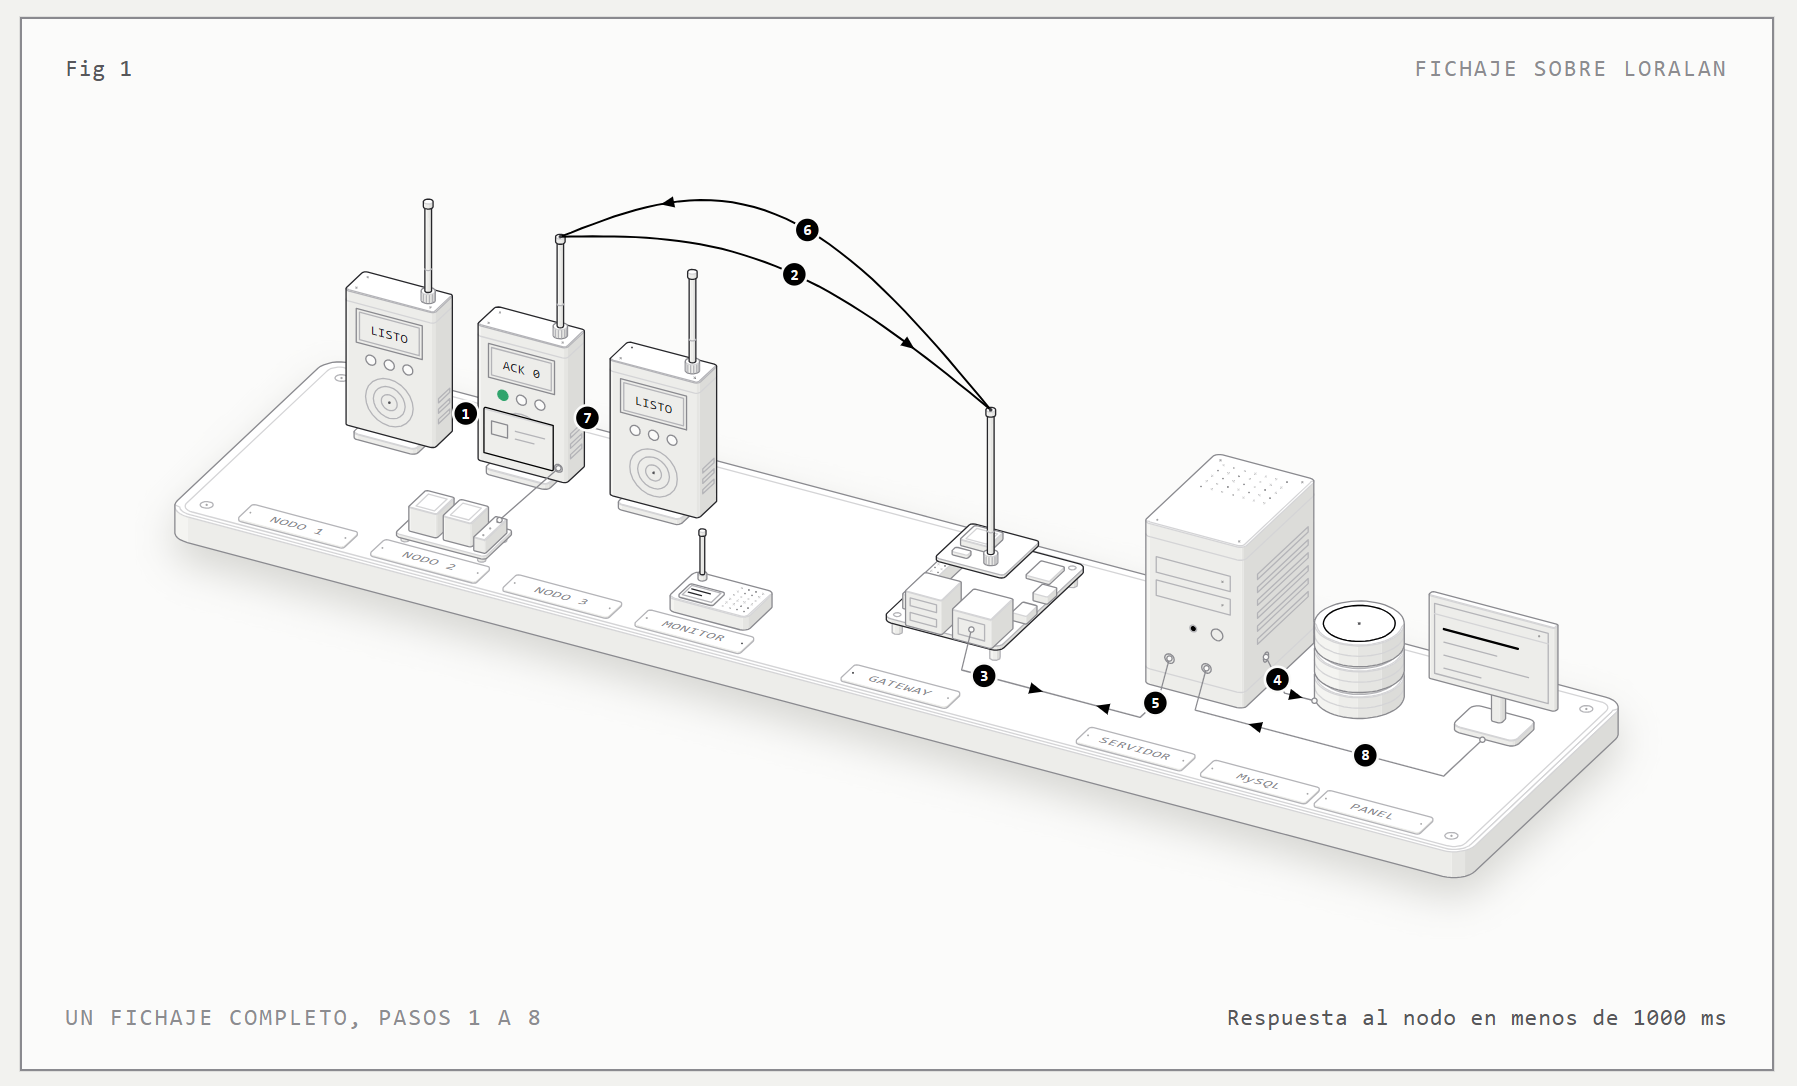
\includegraphics[width=0.92\textwidth]{imagenes/fichajeSatisfecho.png}
\caption{\label{fig:fichaje} Secuencia de un fichaje aceptado.}
\end{figure}

Con SF7, el intercambio de radio consta de dos tramas: 51,5~ms de ida
(identificadores de 4 a 7~bytes) y 41,2~ms de vuelta; el resto depende del
servidor. Para que el nodo reciba siempre una respuesta, se encadenan tres
plazos: la petición HTTP se abandona a los 800~ms, el gateway responde
REINTENTAR a los 1000~ms (descartando respuestas posteriores) y el nodo no
retransmite hasta los 1200~ms. Así, ante un servidor lento o caído, el nodo
obtiene una respuesta explícita en torno a un segundo en lugar de agotar sus
reintentos y ocupar el canal. Los casos de error se resuelven así:

\begin{itemize}
    \item \textbf{Servidor sin respuesta}: el nodo guarda el fichaje en una
    cola en memoria (hasta ocho elementos) y lo reenvía cada 30~s hasta
    obtener un código definitivo, sin que el profesor repita el fichaje.
    \item \textbf{ACK perdido}: el gateway reconoce el número de secuencia de
    la retransmisión y reenvía el mismo ACK sin consultar al servidor.
    \item \textbf{Respuesta tardía del servidor}: el fichaje reenviado ya está
    registrado; el servidor detecta la asistencia existente (profesor, clase
    y aula) y responde OK sin duplicarla.
    \item \textbf{Reinicio del nodo}: los fichajes en cola se pierden al
    residir en memoria volátil, limitación asumida en el prototipo.
\end{itemize}

La fiabilidad de extremo a extremo no depende de una sola capa: LoRaLAN evita
los duplicados de radio y la aplicación, los de aplicación.

\subsection{Telemetría y órdenes}

La telemetría se apoya en el sondeo. Cuando el gateway sondea a un nodo, este responde con el estado de los relés si ha cambiado. Una orden de relé recorre el camino contrario: el panel la envía al servidor, que la encola; el gateway la recoge en su siguiente consulta y la transmite como paquete de tipo CMD; y el nodo actúa sobre la salida e informa de su nuevo estado en el sondeo siguiente. Por tanto, el panel no muestra lo que se ha ordenado, sino lo que el nodo confirma que ha hecho.

\section{Backend FastAPI}

El servidor se organiza en tres capas: los \textit{routers} declaran las operaciones HTTP y validan sus datos con modelos de Pydantic, los servicios contienen la lógica de negocio y los repositorios encapsulan las consultas a la base de datos. Las operaciones se resumen en la Tabla~\ref{tab:endpoints}.

\begin{table}[H]
\centering
\small
\caption{\label{tab:endpoints} Operaciones del servidor.}
\begin{tabular}{|l|l|l|p{6.2cm}|}
\hline
\textbf{Método} & \textbf{Ruta} & \textbf{Rol} & \textbf{Función} \\
\hline
POST & \texttt{/auth/device} & --- & Entrega un \textit{token} al gateway a cambio de su nombre y su clave. \\
\hline
POST & \texttt{/auth/login} & --- & Valida el correo y la contraseña, entrega el \textit{token} del usuario en una \textit{cookie} \texttt{HttpOnly} y lo redirige al panel de su rol. \\
\hline
GET & \texttt{/logout} & --- & Borra la \textit{cookie} de sesión. \\
\hline
POST & \texttt{/gateway/fichaje} & Gateway & Registra un fichaje y devuelve el código de resultado. \\
\hline
POST & \texttt{/gateway/uplink} & Gateway & Recibe sensores, estado de relés y altas/bajas de nodos. \\
\hline
GET & \texttt{/gateway/commands} & Gateway & Entrega y vacía la cola de órdenes del gateway. \\
\hline
POST & \texttt{/gateway/status} & Gateway & Recibe nodos, tráfico, descartes y ciclo de trabajo. \\
\hline
GET & \texttt{/panel/estado} & Conserje, admin. & Estado de las aulas y, para el administrador, de la radio y los gateways. \\
\hline
POST & \texttt{/panel/rele} & Conserje, admin. & Encola una orden de relé. \\
\hline
POST & \texttt{/panel/reset} & Admin. & Encola un reinicio del nodo. \\
\hline
POST & \texttt{/panel/aula} & Admin. & Asigna un aula a un nodo. \\
\hline
\end{tabular}
\end{table}

La operación de fichaje responde siempre con éxito HTTP y devuelve el resultado en el campo \texttt{code}, puesto que el gateway necesita un byte para el ACK y no un estado que interpretar. Para decidirlo, el servidor busca al profesor por la tarjeta y el aula asignada al nodo, y responde DESCONOCIDO si falta alguno; busca después la clase de esa aula en ese momento, primero en la base de datos y, si no la encuentra, consulta el servicio de reservas de la universidad. Responde SIN\_CLASE si no la hay o DENEGADO si es de otro profesor; y, por último, registra la asistencia salvo que ya exista una de ese profesor en esa clase y esa aula, respondiendo OK en ambos casos. Cualquier error interno se traduce en REINTENTAR y nunca en un código definitivo, que haría que el nodo descartase un fichaje legítimo.

En cuanto a la autenticación, el servidor emite \textit{tokens} JWT para dos tipos de cliente. Las personas inician sesión con su correo y una contraseña almacenada como \textit{hash} bcrypt, y su \textit{token} viaja en una \textit{cookie} \texttt{HttpOnly} que se comprueba en cada operación según el rol, mientras que el gateway presenta un \textit{token} de dispositivo que renueva cuando caduca. El servidor comprueba además que el gateway nombrado en cada petición coincide con el del \textit{token}, impide que un nodo del sistema antiguo actúe como gateway y limita los intentos de autenticación por dirección IP.

El último estado de cada aula y la cola de órdenes se mantienen en memoria, y un nodo se considera conectado si el gateway ha subido algo suyo en los últimos 120~segundos. Un reinicio del servidor pierde, por tanto, las órdenes no recogidas, aunque el estado se reconstruye con los siguientes sondeos. Los paneles consultan ese estado cada 5~segundos: el conserje ve las aulas y acciona sus relés, y el administrador ve además los datos de radio de cada nodo y el consumo de ciclo de trabajo de los gateways.

\section{Base de datos}

La base de datos consta de las cinco tablas que se muestran en el diagrama entidad-relación de la Figura~\ref{fig:er}.

\begin{figure}[H]
\centering
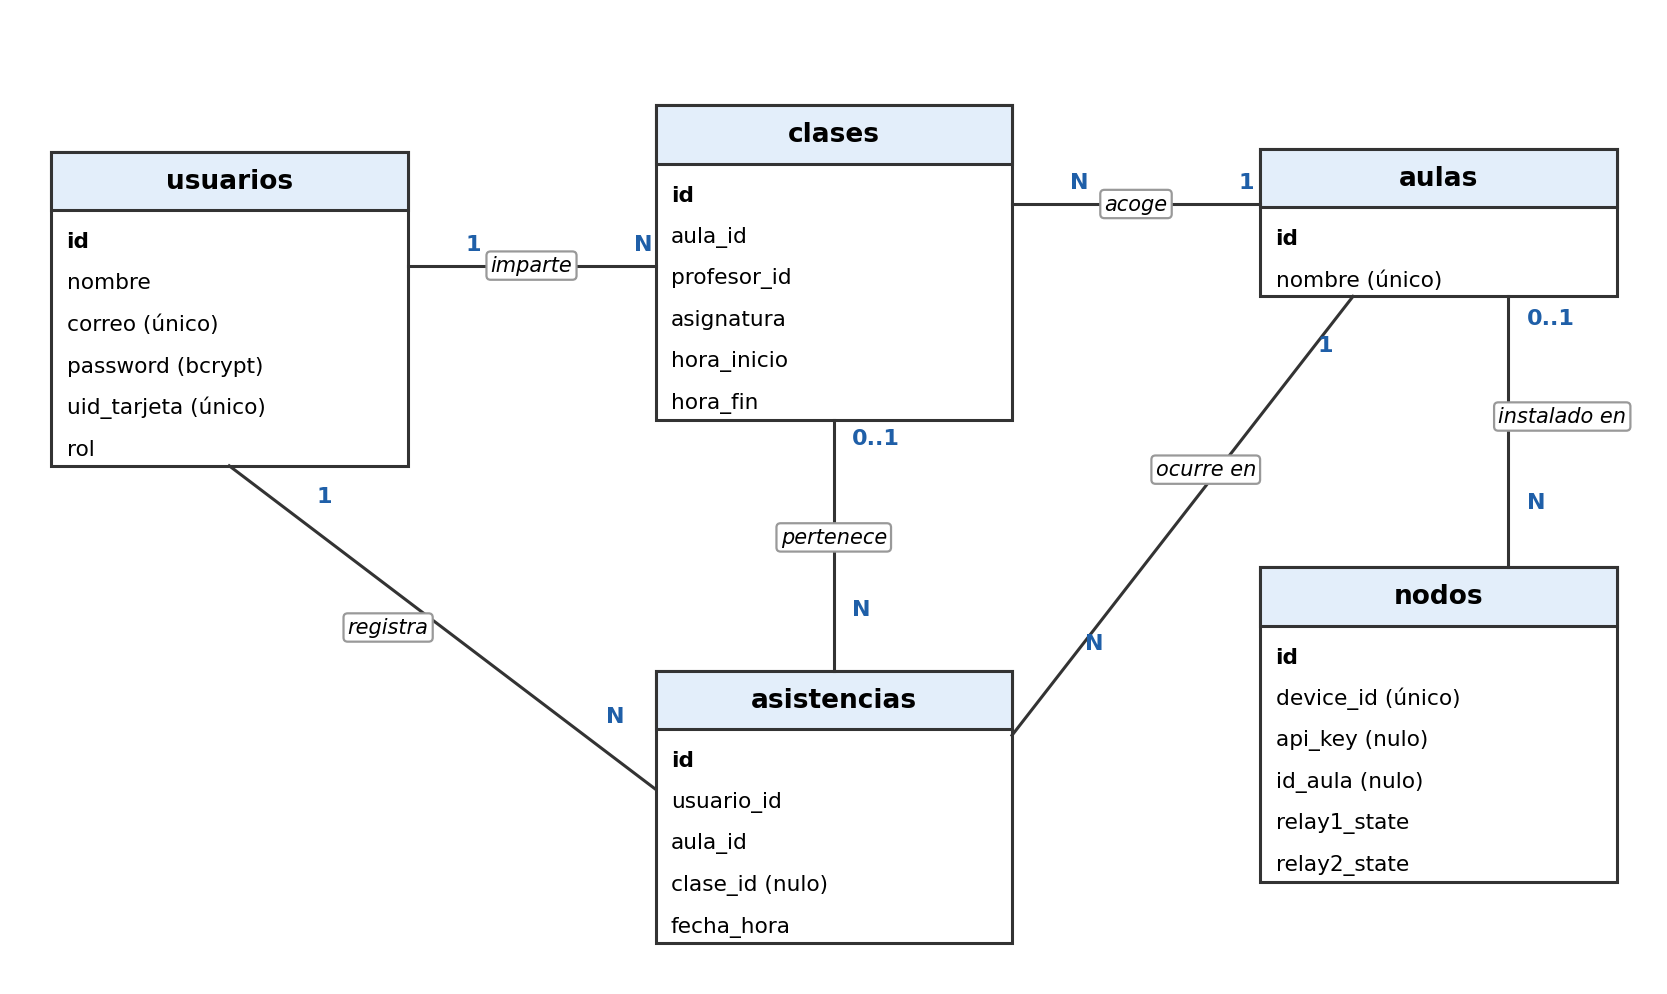
\includegraphics[width=0.9\textwidth]{imagenes/er_fichaje.png}
\caption{\label{fig:er} Diagrama entidad-relación de la base de datos del sistema de la aplicación.}
\end{figure}

La tabla de usuarios recoge profesores, conserjes y administradores. Aulas identifica las aulas por un nombre único. Clases relaciona profesores, aulas y franjas horarias. Asistencias registra los fichajes aceptados y nodos almacena los dispositivos LoRaLAN y gateways, junto con su identificación, aula asignada y estado de los relés.
Las claves ajenas mantienen la integridad referencial, con dos excepciones deliberadas: al eliminar un aula, sus nodos quedan sin asignación, y al eliminar una clase se conservan las asistencias asociadas. Los nodos se registran automáticamente al recibir su primer paquete y, hasta que el administrador les asigna un aula, sus fichajes reciben el código DESCONOCIDO.


\section{Diseño de la PCB del nodo}\label{sec:pcb}

Las pruebas descritas hasta ahora se realizaron con placas de desarrollo conectadas mediante cableado utilizando una protoboard, una solución adecuada para validar el funcionamiento, pero poco robusta y difícil de replicar en un despliegue real. Además, trabajar sobre una protoboard implica trabajar, habitualmente, con cables que no hacen bien contacto y problemas de conexión que a menudo se solventan asegurando que los cables hacen contacto en sus pines.


Por este motivo, se ha diseñado una placa de circuito impreso (PCB) específica para el nodo LoRaLAN en esta aplicación, que integra en un único soporte las conexiones de todos los componentes.

El diseño se ha realizado con EasyEDA, una herramienta de diseño electrónico que integra en un mismo entorno la captura del esquemático, el diseño de la placa y la generación de los ficheros de fabricación. Además, su biblioteca de componentes hechos por la comunidad permite utilizar casi cualquier componente y cualquier configuración que pueda existir de dicho componente, lo que reduce los errores al pasar del esquemático a la placa y facilita su fabricación por un proveedor externo.

El esquemático, recogido en la Figura~\ref{fig:pcb1}, es el primer paso para generar una PCB. En él se agregan todos los componentes y se realiza el cableado de todos los elementos.

\begin{figure}[H]
\centering
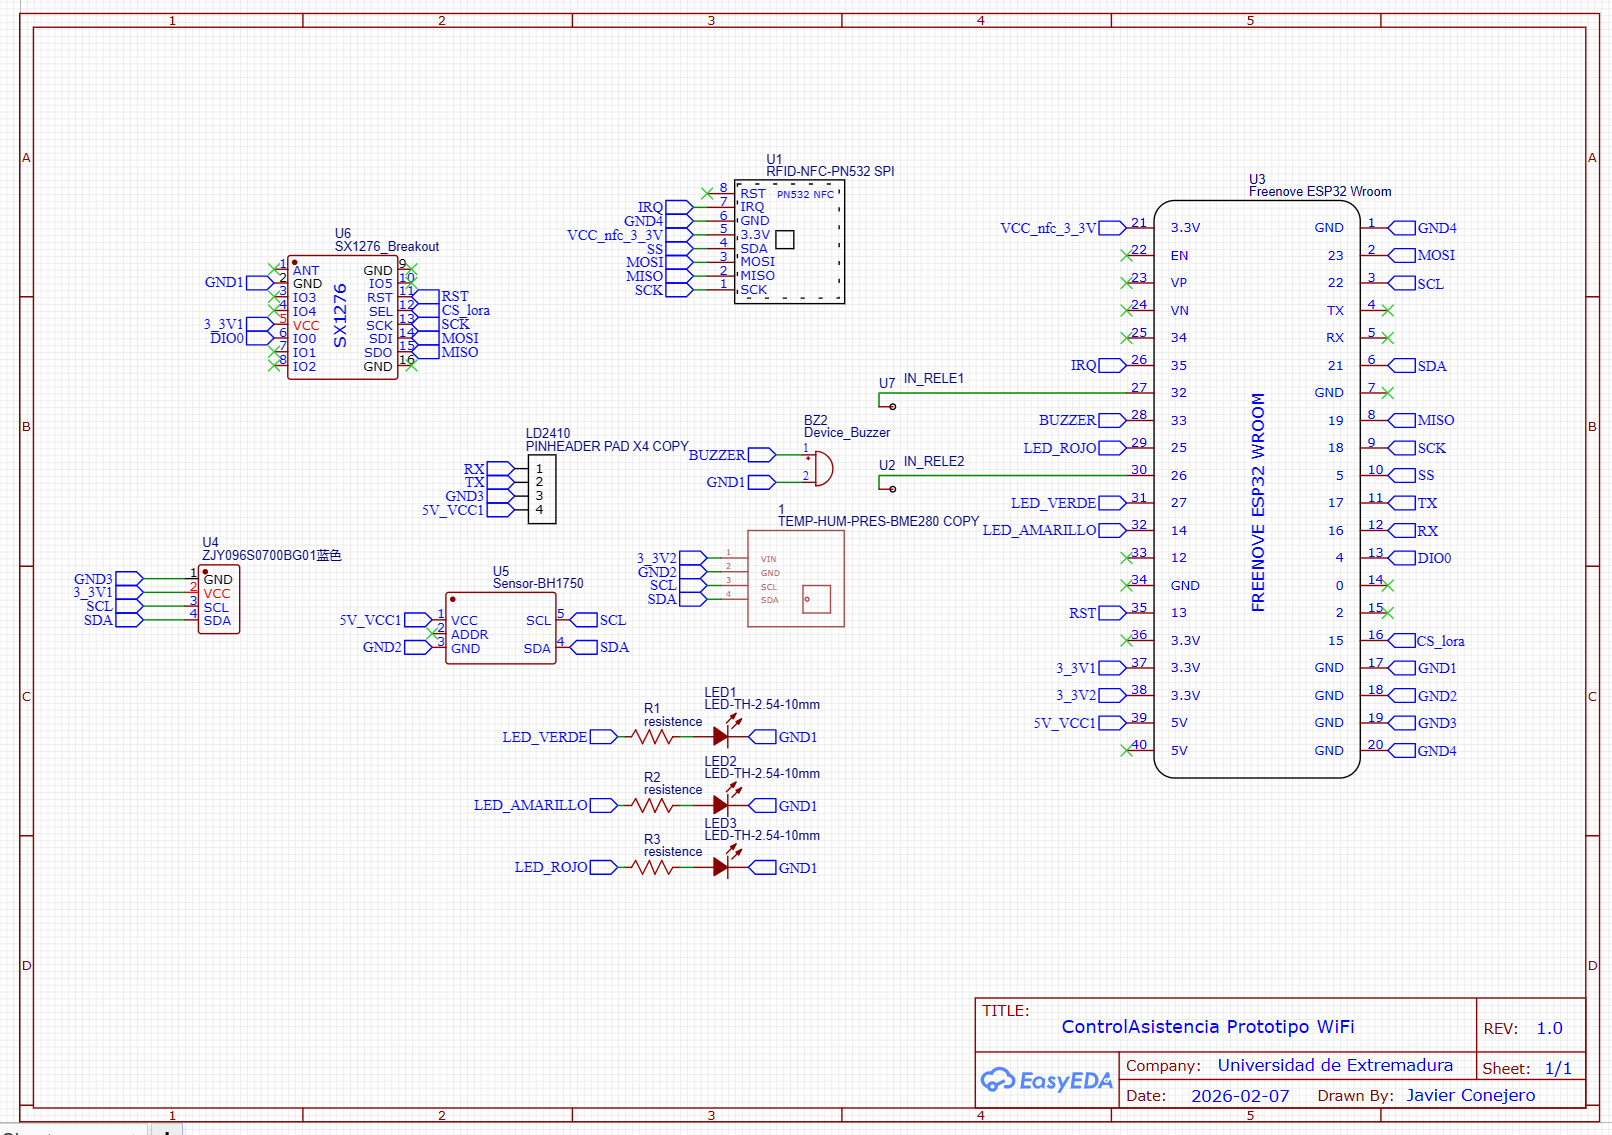
\includegraphics[width=0.9\textwidth]{imagenes/pcb-esquematico.png}
\caption{\label{fig:pcb1} Diagrama de cableado del prototipo de Registro de asistencia.}
\end{figure}

Posteriormente se validan las conexiones del esquemático mediante la comprobación de reglas eléctricas (ERC) y se revisan los \textit{warnings} que aparecen, antes de generar la propia PCB. A continuación se pulsa la opción " Convertir a PCB".

\begin{figure}[H]
\centering
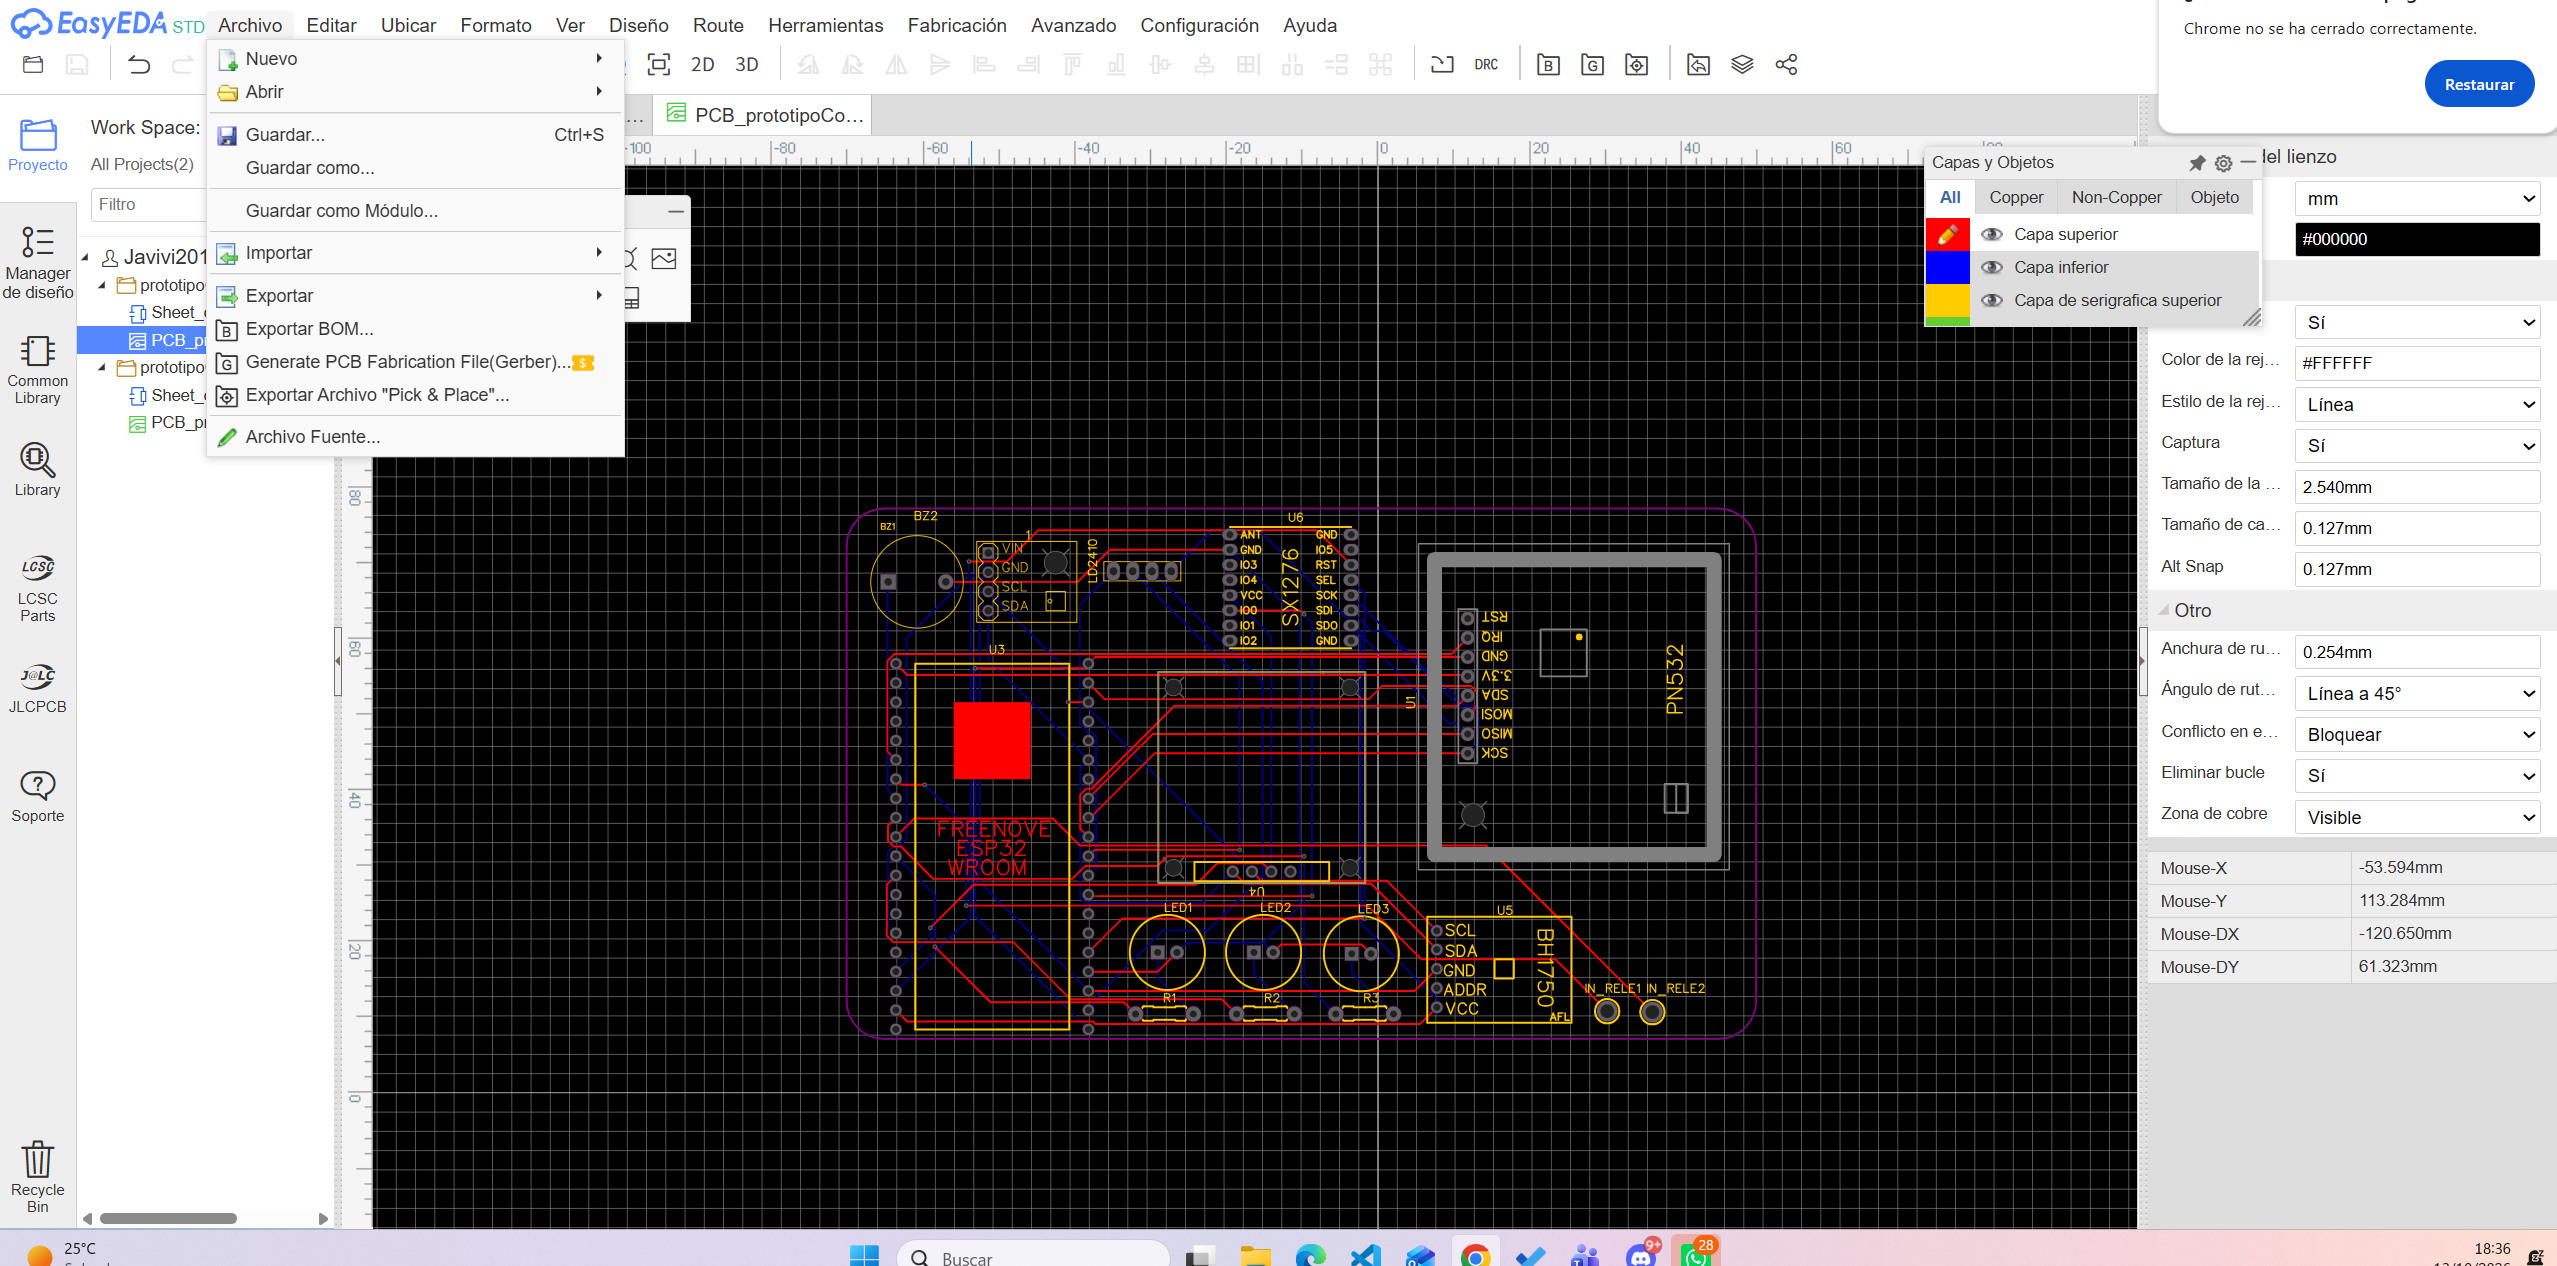
\includegraphics[width=0.9\textwidth]{imagenes/pcb-esquematico2.png}
\caption{\label{fig:pcb2} Previsualización de la PCB de Registro de asistencia.}
\end{figure}

Tal y como se muestra en la Figura~\ref{fig:pcb2}, en esta pantalla se determina cuáles son las dimensiones de la PCB y se posicionan los componentes como se desee. En este caso, se han posicionado todos los elementos intentando minimizar la dimensión de la PCB.

Posteriormente, se utiliza la herramienta auto-ruteo que se encarga de posicionar las pistas sobre las capas de la placa, de manera que no se crucen las pistas entre sí. Además, se tuvo en cuenta que el PN532 debe estar lo más aislado posible, para que no genere interferencias electromagnéticas, dando lugar a errores de lectura.

Por otro lado, el transceptor y la antena se sitúan en un extremo de la placa de forma que la antena sobresalga lo máximo posible para limitar las pérdidas y las interferencias. Por último, se agrega un plano de masa para proporcionar una referencia de 0 V sólida, ofrecer un camino de retorno de corriente de baja impedancia y reducir las interferencias electromagnéticas.


Finalmente, a partir del diseño se mandó fabricar la placa a través de JLCPCB, el fabricante asociado a EasyEDA. En la Figura~\ref{fig:pcb3} se muestra la apariencia final de la PCB.

\begin{figure}[H]
\centering
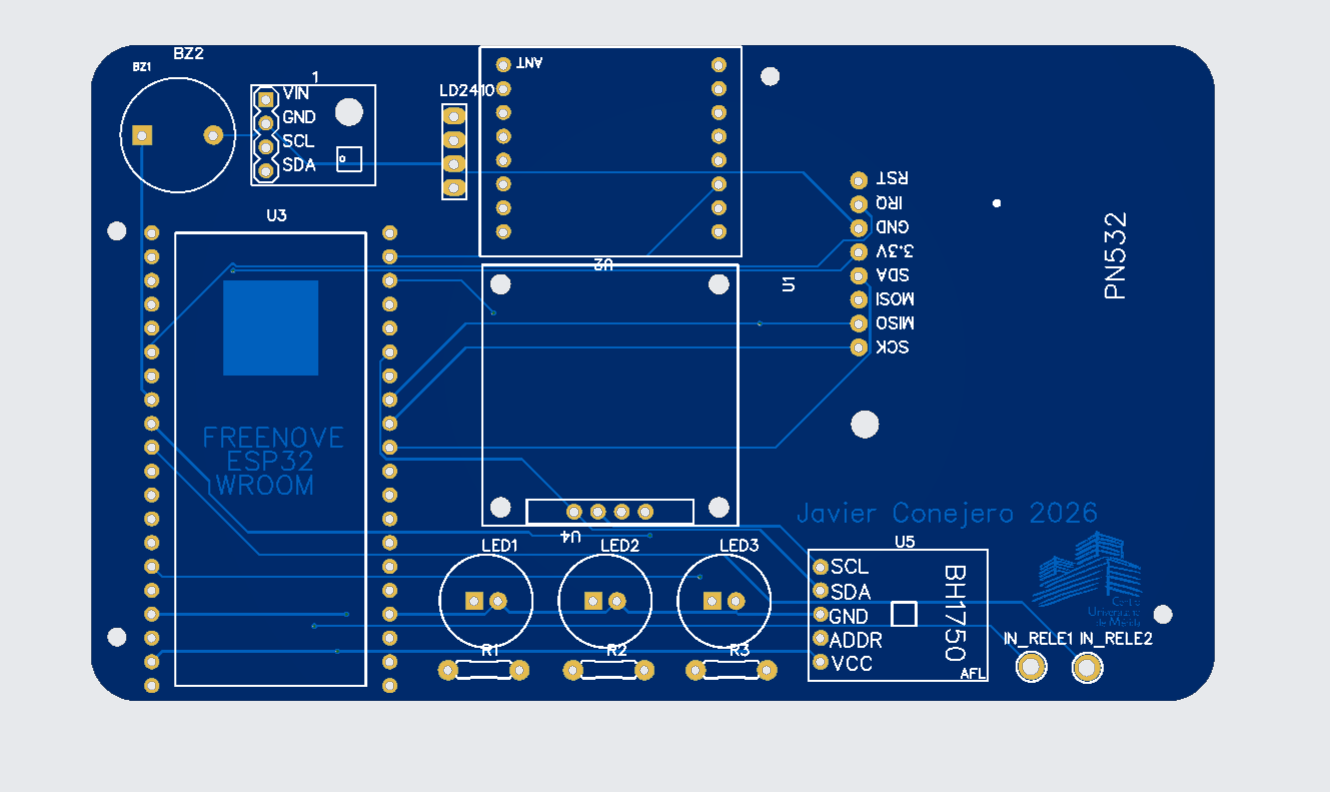
\includegraphics[width=0.9\textwidth]{imagenes/pcb.png}
\caption{\label{fig:pcb3} Resultado final del diseño de la PCB.}
\end{figure}

Esta placa convierte el prototipo en un dispositivo compacto y replicable, preparado para el despliegue de varios nodos.



\section{Monitor de red Cardputer M5}

Además de probar el sistema completo sobre hardware, con un nodo de aula con todos sus periféricos, el gateway y el servidor en una Raspberry Pi, la base de datos en otro equipo, se decide implementar un monitor de red para poder consultar el tráfico de la red LoRaLAN en tiempo real. Para ello, se implementó el monitor de red sobre un Cardputer M5 con el módulo SX1262. En la Figura~\ref{fig:cardputer1} se muestra un ejemplo de funcionamiento del monitor de red con un nodo conectado, donde se observan parámetros del nodo.


\begin{figure}[H]
\centering
        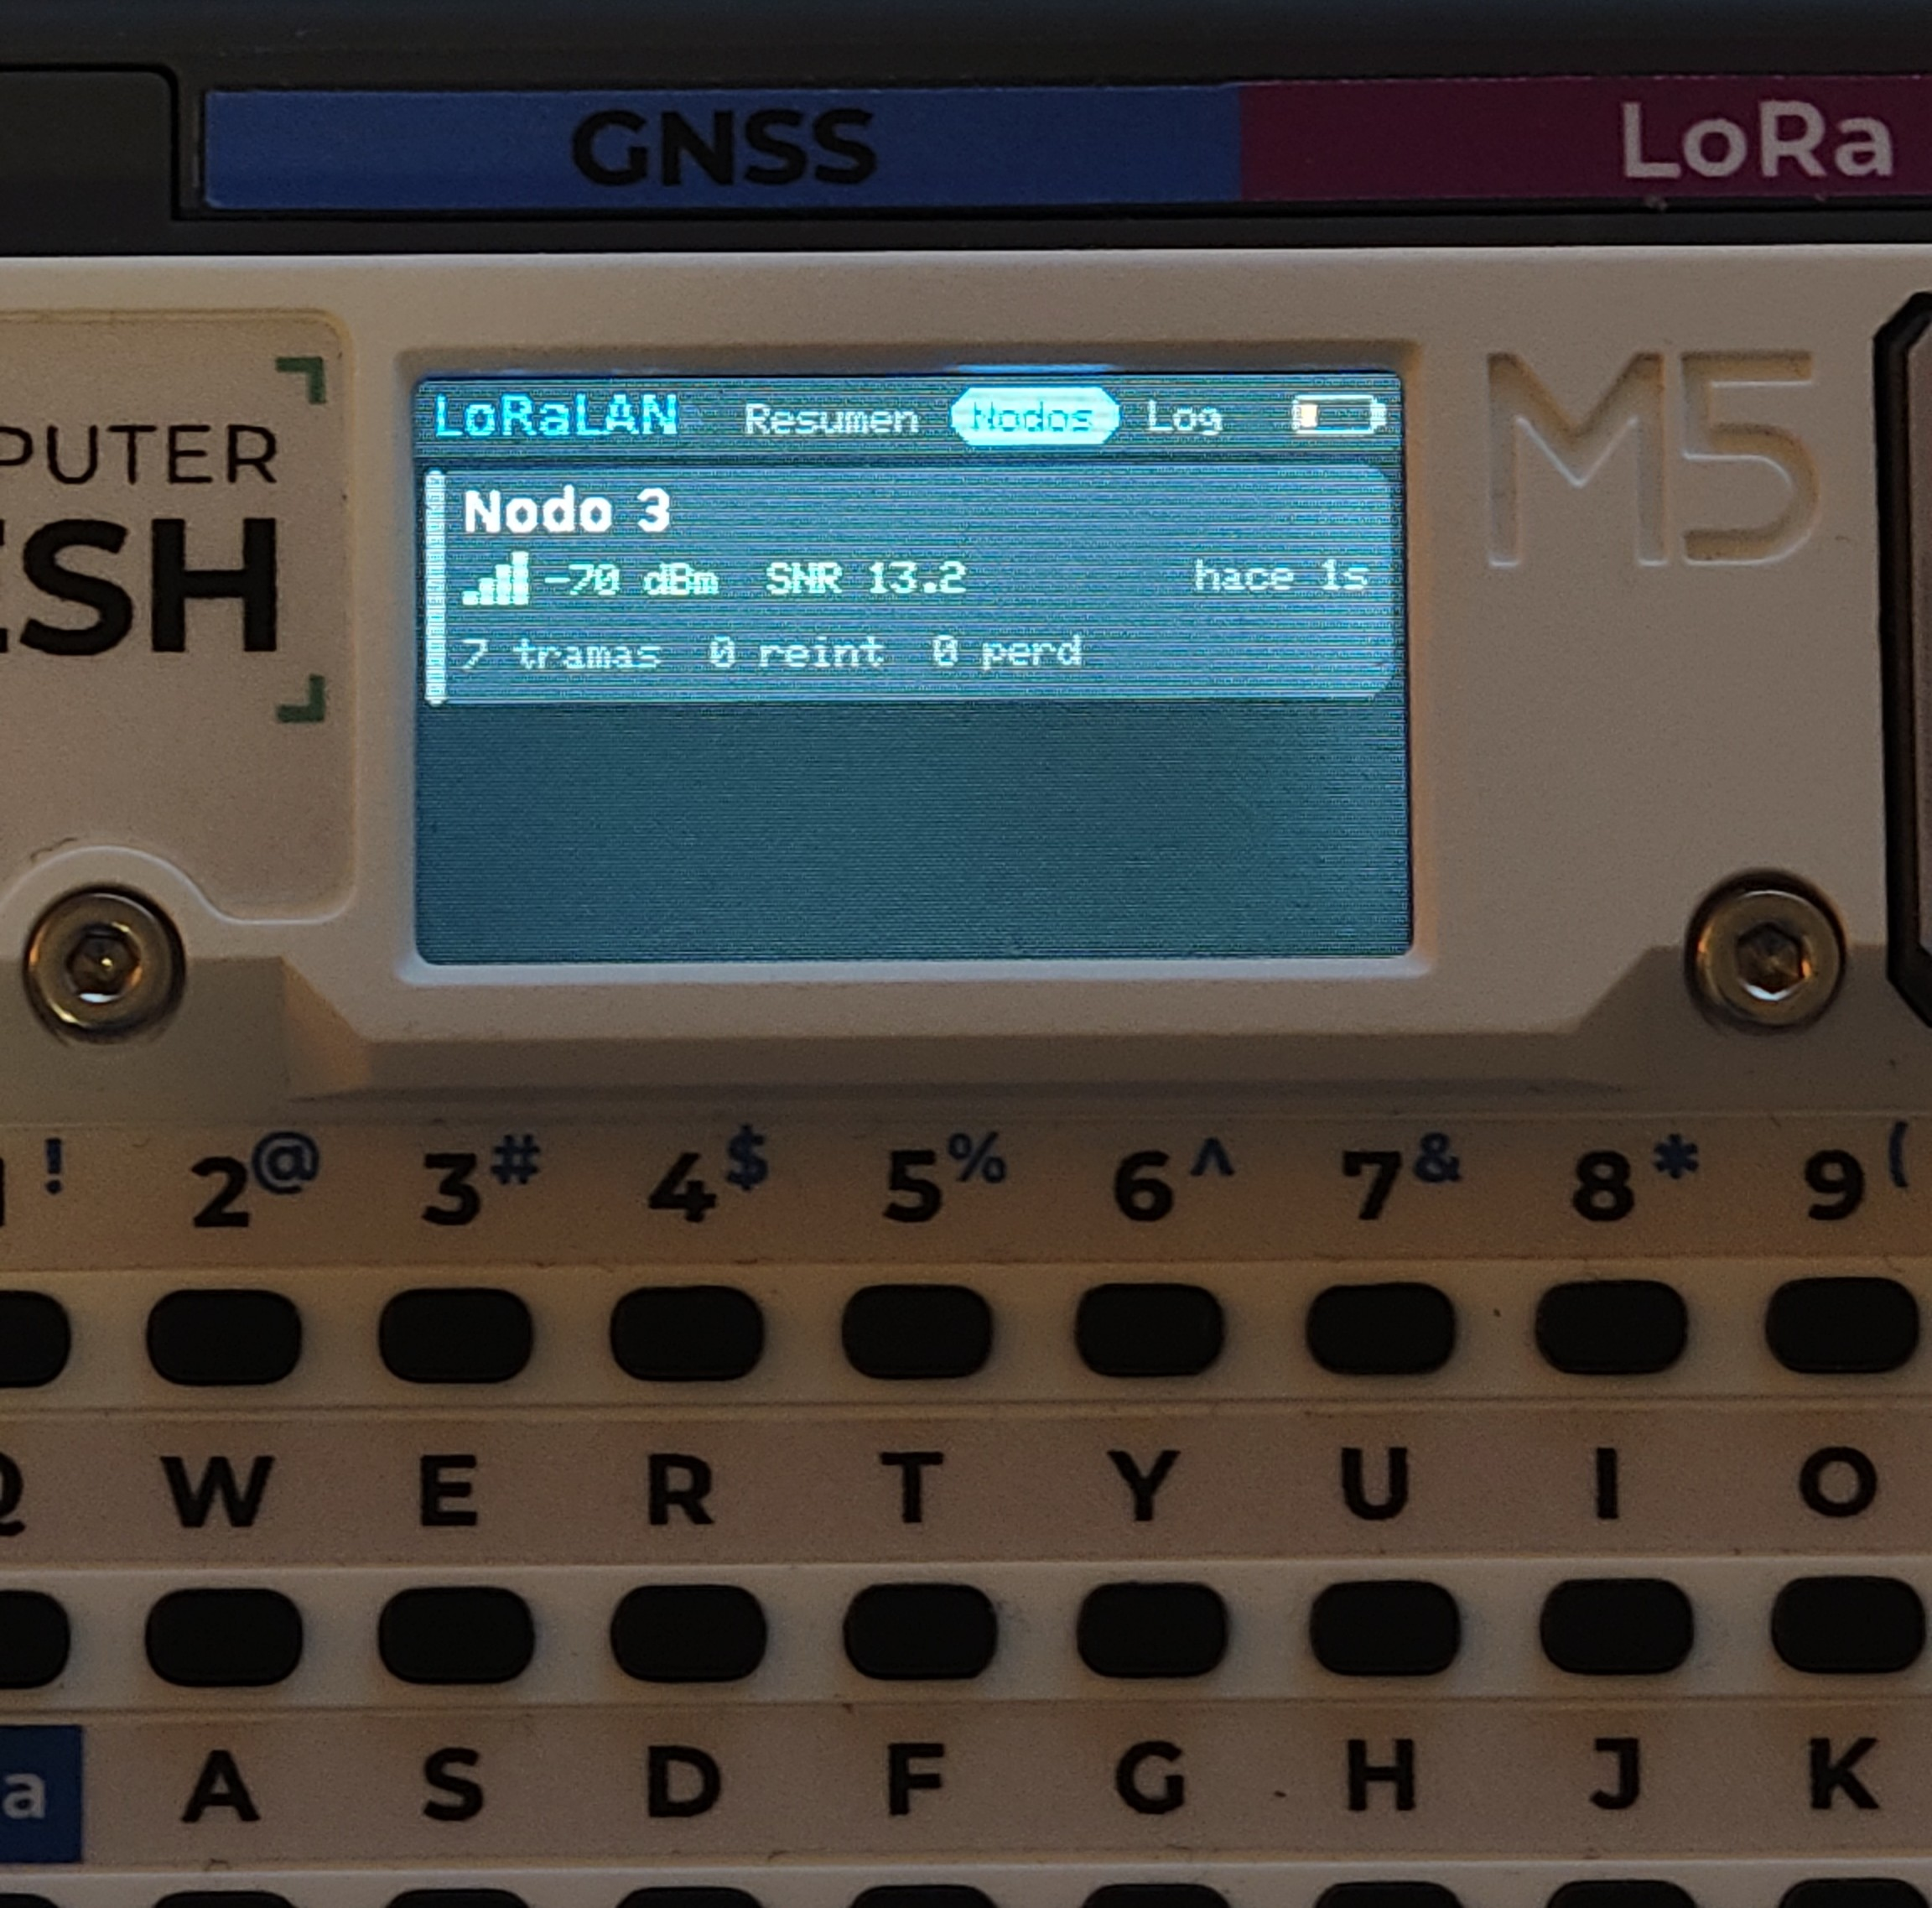
\includegraphics[width=0.8\textwidth]{imagenes/cardputer.jpg}
        \caption{Panel del monitor de red que muestra los nodos y algunos parámetros.}
        \label{fig:cardputer1}
\end{figure}

Se ha utilizado la placa LILYGO TTGO LoRa32 como hardware adicional para evaluar el comportamiento de la aplicación en hardware real. En este caso, se emplea la placa LILYGO con una versión modificada del firmware del nodo de aula, que funciona exactamente igual que el original, pero en lugar de poseer sensores y realizar lecturas sobre ellos, simula el envío de esta información. De esta manera se puede evaluar el funcionamiento del prototipo con dos nodos y un gateway y ver cómo se comporta la red con Cardputer.

\begin{figure}[H]
        \centering
        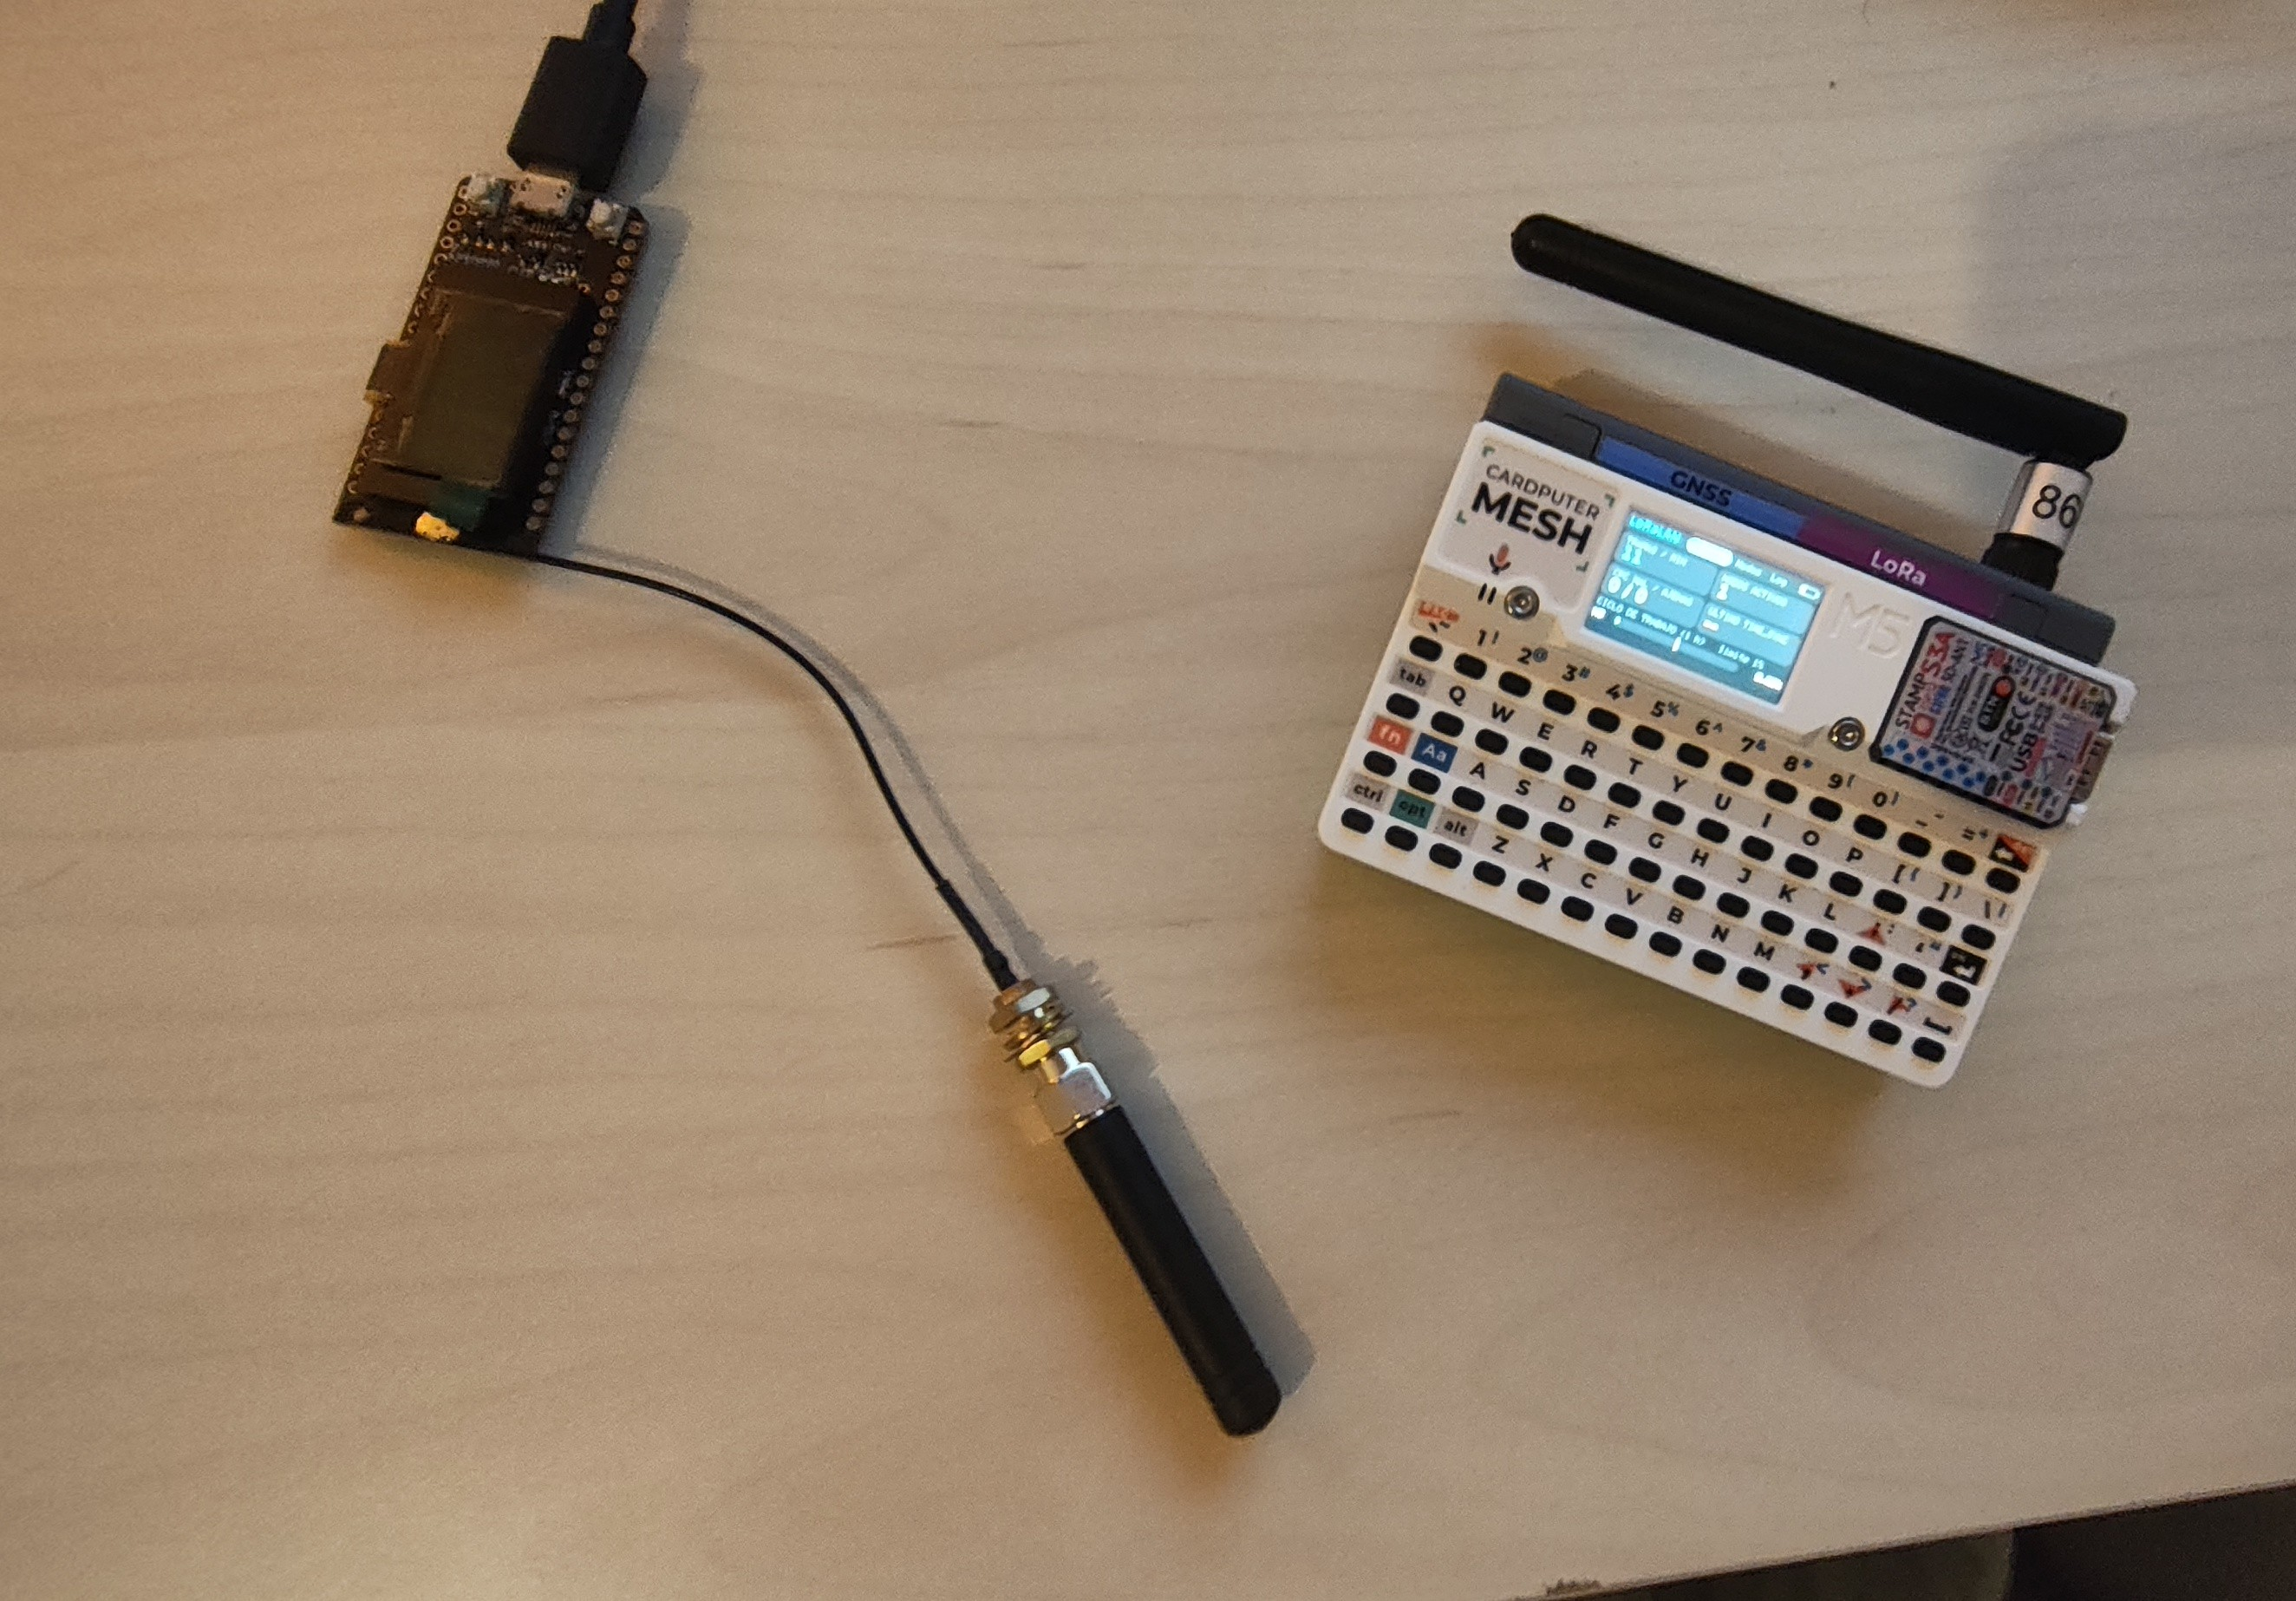
\includegraphics[width=1\textwidth]{imagenes/cardputer2.jpg}
        \caption{Monitor de red Cardputer y nodo simulado Lilygo.}
        \label{fig:imagen2}
\end{figure}





\section{Pruebas del sistema}

El sistema completo se ha probado además sobre hardware real, con un nodo de aula con todos sus periféricos, el gateway y el servidor en una Raspberry Pi, la base de datos en otro equipo y el monitor de red como observador independiente. Los escenarios ejercitados se muestran en la Tabla~\ref{tab:e2e}.

\begin{table}[H]
\centering
\small
\caption{\label{tab:e2e} Escenarios de la prueba de extremo a extremo.}
\begin{tabular}{|c|p{5.2cm}|p{7.8cm}|}
\hline
\textbf{N.º} & \textbf{Escenario} & \textbf{Resultado esperado} \\
\hline
1 & Arranque del nodo & Se asocia y el servidor lo da de alta. \\
\hline
2 & Tarjeta válida con clase & LED verde y nueva fila en la tabla de asistencias. \\
\hline
3 & Tarjeta desconocida & LED rojo y ningún registro. \\
\hline
4 & Fichaje con el servidor detenido & El nodo indica reintento y el fichaje se registra una sola vez al volver el servidor. \\
\hline
5 & Orden de relé desde el panel & El relé conmuta en pocos segundos y el panel refleja el nuevo estado. \\
\hline
6 & Supervisión & El panel muestra los sensores del aula. \\
\hline
7 & Reinicio de nodo & Desde el panel web por parte del administrador se envía la petición de reinicio a un nodo. \\
\hline
\end{tabular}
\end{table}

El sistema funcionó de extremo a extremo, de modo que los fichajes, la telemetría y las órdenes recorrieron la cadena completa.


\chapter{Conclusiones y trabajo futuro}\label{chap:8}

En este capítulo se recogen las conclusiones a partir de los resultados obtenidos y se proponen las líneas de trabajo futuro.

\section{Conclusiones}

Las conclusiones tras el diseño, desarrollo y evaluación del protocolo LoRaLAN son las siguientes:

\begin{itemize}

\item \textbf{Viabilidad del protocolo}: Se ha diseñado e implementado LoRaLAN como un protocolo de comunicación de área local sobre LoRa, adaptado a redes de sensores y dispositivos con requisitos de bajo consumo y tráfico reducido. Los resultados de simulación muestran tasas estimadas de entrega del 99,5\,\% con un 20\,\% de pérdidas en el canal y superiores al 99,8\,\% con una mayor carga de red, en redes con distinta cantidad de nodos registrados.

\item \textbf{Portabilidad de la implementación}: La separación entre la lógica del protocolo y las operaciones dependientes de la plataforma ha permitido desarrollar una biblioteca común para ESP32, Raspberry Pi y simulador de PC. Esta arquitectura facilita su mantenimiento, reutilización y adaptación a distintos dispositivos sin duplicar la implementación del protocolo.

\item \textbf{Validación y alcance del simulador}: Se ha desarrollado un entorno de simulación reproducible que permite evaluar el comportamiento de la red ante pérdidas, retrasos, duplicaciones, reordenamientos y corrupción de tramas. La batería de casos ha permitido identificar defectos durante el desarrollo y verificar buena parte de los requisitos. No obstante, los resultados no sustituyen a las pruebas radioeléctricas reales, especialmente en lo relativo al alcance, las interferencias y los tiempos de comunicación, que se asumen en cierto modo ya que dependen principalmente del comportamiento de LoRa.

\item \textbf{Viabilidad de la aplicación desarrollada}: La integración de LoRaLAN en un sistema de registro de asistencia mediante NFC y monitorización de aulas ha demostrado su utilidad en un escenario real. El conjunto ha funcionado correctamente de extremo a extremo con un nodo físico y uno simulado, pero no ha sido posible validar el funcionamiento del protocolo en un entorno real con varios nodos en funcionamiento.

\item \textbf{Adecuación a las restricciones radioeléctricas}: Las mediciones mediante SDR y el análisis del tráfico generado han permitido estudiar la ocupación de la banda seleccionada en el Centro Universitario de Mérida y estimar el cumplimiento de las restricciones de ciclo de trabajo. Los resultados analíticos y de simulación indican que la configuración planteada se mantiene dentro del límite del 10\,\% por hora, aunque su confirmación definitiva requiere completar las mediciones de tiempo en el aire sobre el hardware.

\item \textbf{Limitaciones y seguridad}: La evaluación ha desvelado que la implementación no satisface todavía todos los requisitos definidos, especialmente los relacionados con los eventos asíncronos, la confirmación de entrega, la baja de nodos y la seguridad. En particular, se ha identificado una vulnerabilidad de repetición de asociaciones antiguas y se ha constatado el riesgo que supone compartir una misma clave maestra entre todos los dispositivos. Estos aspectos delimitan el alcance actual de LoRaLAN y constituyen prioridades para futuras mejoras.

\item \textbf{Flexibilidad de LoRa como soporte de protocolos propios}: El trabajo demuestra que es posible utilizar LoRa como capa física para desarrollar un protocolo adaptado a las necesidades de una aplicación concreta, definiendo los mecanismos de acceso al medio, direccionamiento, gestión de nodos y seguridad. En este caso, la combinación de sondeo periódico y eventos asíncronos permite atender tanto la monitorización como los fichajes, manteniendo el control de las comunicaciones en la propia aplicación y sin depender de un servidor de red externo.

\end{itemize}

Como conclusión general, se puede afirmar que el trabajo ha alcanzado su objetivo principal, que consistía en diseñar un protocolo de red local sobre LoRa ajustado a un problema concreto y en demostrar su utilidad mediante una aplicación real. Además, LoRaLAN es una propuesta que ofrece algo distinto al resto de protocolos y soluciones actuales sobre LoRa. Ofrece una alternativa descentralizada y privada, donde se da la libertad total al programador de crear su aplicación de IoT, sin necesidad de conexión a internet, sin depender de una infraestructura gestionada por terceros, que ofrece versatilidad a la hora de programar el tipo de tráfico que la red va a gestionar y que es independiente del hardware.
 
En este caso, sobre esta base se construyó un sistema de registro de asistencia por NFC y monitoreo de aulas para los docentes del Centro Universitario de Mérida que funcionó de extremo a extremo sobre hardware real y que muestra una alternativa para prescindir de la red Wi-Fi del edificio a la hora de ofrecer servicios novedosos que simplifican las labores de los docentes y de los conserjes.
  
\section{Trabajo futuro}


A partir de los resultados obtenidos y de las limitaciones identificadas, se plantean las siguientes líneas de trabajo futuro:

\begin{itemize}
    \item \textbf{Mejora del acceso al medio}: Incorporar escucha previa en las emisiones periódicas del gateway y adaptar el sondeo para evitar que interfiera con intercambios en curso. Asimismo, podría implementarse un sondeo adaptativo que priorice los nodos con actividad reciente o con órdenes pendientes.

    \item \textbf{Mayor robustez del protocolo}: Admitir varias cargas pendientes en el nodo y garantizar su cancelación al producirse una baja, y mejorar la recuperación tras un reinicio del gateway mediante un mecanismo de aviso que permita la reasociación inmediata.

    \item \textbf{Refuerzo de los mecanismos de seguridad}: Corregir la vulnerabilidad detectada en el proceso de asociación mediante mecanismos que impidan la reutilización de asociaciones y claves de sesión antiguas y estudiar la sustitución de la clave maestra compartida por un esquema de claves independientes por nodo, de forma que el compromiso de un dispositivo no afecte a la seguridad del resto de la red.

    \item \textbf{Optimización del consumo energético}: Incorporar un modo de bajo consumo que permita a los nodos permanecer dormidos y limitar sus periodos de escucha.

    \item \textbf{Validación experimental en hardware}: Realizar una prueba de despliegue con varias placas para caracterizar los tiempos de transmisión e ida y vuelta, la ventana ciega, la eficacia de la escucha previa, el alcance, la calidad de señal y las tasas de entrega y latencia, con ayuda de herramientas como el SDR.

    \item \textbf{Despliegue piloto}: Instalar el sistema en varias aulas durante un periodo lectivo, evaluando su funcionamiento en condiciones reales y determinando las necesidades de cobertura y coordinación entre el gateway y los nodos para un posible despliegue.
\end{itemize}
% etc...

%----------------------------------------------------
% INCLUIMOS LOS ANEXOS (SI ES NECESARIO)
\appendix
\clearpage
\addappheadtotoc
\appendixpage
\chapter{Catálogo de pruebas funcionales evaluadas}\label{anexo_A}
En este anexo se recoge en la tabla \ref{tab:catalogo} la descripción detallada de las pruebas funcionales diseñadas para verificar el protocolo.

{\small
\begin{longtable}{|c|p{6.4cm}|p{6.8cm}|}
\caption{\label{tab:catalogo} Catálogo de pruebas de formato y de protocolo.}\\
\hline
\textbf{Id} & \textbf{Situación} & \textbf{Resultado esperado} \\
\hline
\endfirsthead
\hline
\textbf{Id} & \textbf{Situación} & \textbf{Resultado esperado} \\
\hline
\endhead
\multicolumn{3}{|l|}{\textbf{Formato de trama}} \\
\hline
F1 & Construir una trama de cada tipo y volver a leerla & Se obtiene lo mismo que se construyó \\
\hline
F2 & Longitudes de 10, 11, 75 y 76~bytes & Solo se aceptan de 11 a 75~bytes \\
\hline
F3 & Secuencia de 16~bits hasta 0xFFFF y paso a 0 & La detección de repeticiones sigue funcionando \\
\hline
F4 & Alterar cada byte de una trama, de uno en uno & El MIC deja de coincidir en todos los casos \\
\hline
F5 & Versión, tipo, prioridad o indicadores inválidos & Trama rechazada, sin caída \\
\hline
F6 & Carga de 0, 1, 64 y 65~bytes & Se acepta hasta 64; se rechaza 65 \\
\hline
\multicolumn{3}{|l|}{\textbf{JOIN}} \\
\hline
J1 & Asociación con el canal limpio & Asociado; un aviso en cada extremo \\
\hline
J2 & Se pierde el JOIN\_REQUEST & Lo repite más tarde con otro DevNonce \\
\hline
J3 & Se pierde el JOIN\_ACCEPT & Repite; el gateway reutiliza entrada y dirección; ambos acaban con la misma clave \\
\hline
J4 & Canal ocupado al solicitar la asociación & No transmite; reintenta después \\
\hline
J5 & Varios nodos se asocian a la vez & Todos asociados, cada uno con su dirección \\
\hline
J6 & El nodo se reinicia con la sesión viva & Sesión nueva; la secuencia se reinicia \\
\hline
J7 & Clave maestra incorrecta & Nunca asociado; sin estado en el gateway \\
\hline
J8 & Otro identificador de red & Se ignora \\
\hline
J9 & Nodo número 33 con la tabla llena & Rechazado; los otros 32 no se ven afectados \\
\hline
J10 & Dirección ocupada o sin preferencia & Recibe otra libre del rango dinámico \\
\hline
J12 & Repetición del último JOIN & Rechazada; la sesión sigue intacta \\
\hline
J13$^{\dagger}$ & Repetición de un JOIN antiguo & Rechazada \\
\hline
J15 & Encolar un evento antes de asociarse & \texttt{queuePushEvent} devuelve \texttt{false} \\
\hline
\multicolumn{3}{|l|}{\textbf{LEAVE}} \\
\hline
L1 & Baja con el canal limpio & ACK; clave borrada; un aviso; no se reasocia solo \\
\hline
L2 & Se pierde el ACK de la baja & Repite; el gateway avisa una vez; acaba de baja \\
\hline
L3 & Se pierden todos los LEAVE & Baja local; el gateway acaba viéndolo inactivo \\
\hline
L4$^{\dagger}$ & Baja mientras el nodo espera la confirmación de otro envío & \texttt{leave()} devuelve \texttt{false} y el nodo sigue asociado \\
\hline
L5$^{\dagger}$ & Baja con un evento pendiente de enviar & El evento se descarta y se avisa a la aplicación con \texttt{delivered=false} \\
\hline
L6 & POLL o CMD durante la baja & Ni responde ni ejecuta \\
\hline
L7 & Reasociación tras la baja & Sesión nueva, misma dirección \\
\hline
L9 & Baja de un nodo entre varios & El sondeo lo salta; los demás no se ven afectados \\
\hline
L10$^{\dagger}$ & Repetición de un LEAVE & Rechazada \\
\hline
\multicolumn{3}{|l|}{\textbf{POLL}} \\
\hline
P1 & POLL sin datos & Respuesta vacía, una vez, sin ACK \\
\hline
P2 & Respuesta generada bajo demanda & Una emisión, sin ACK \\
\hline
P3 & Carga con ACK & Se confirma y se borra del nodo \\
\hline
P4 & Carga con ACK; se pierde el ACK & Se conserva y se repite después \\
\hline
P5 & Carga sin ACK & Una emisión y se borra \\
\hline
P6$^{\dagger}$ & Preparar una respuesta de sondeo cuando ya hay otra pendiente & \texttt{queuePollPayload} devuelve \texttt{false} y conserva la anterior \\
\hline
P7 & POLL dirigido a otro nodo & No responde \\
\hline
P8 & Se pierde el POLL & Aumentan los sondeos sin respuesta; llega el siguiente turno \\
\hline
P9 & Se pierde la POLL\_RESPONSE & Sin ACK, dato perdido; con ACK, se repite \\
\hline
P10 & Varios nodos & Turnos justos; cada nodo, cada $N$ intervalos \\
\hline
P11 & Un nodo deja de contestar y vuelve & Un aviso de inactivo; se sigue sondeando; se reactiva \\
\hline
P14$^{\dagger}$ & Llega un POLL mientras el nodo espera un ACK & Responder al POLL no impide recibir ese ACK \\
\hline
\multicolumn{3}{|l|}{\textbf{PUSH}} \\
\hline
U1 & Evento en reposo con el canal libre & Una escucha y una emisión; llega en un tiempo en el aire \\
\hline
U2 & Evento sin ACK & Una emisión, sin ACK \\
\hline
U3 & Canal ocupado & Espera creciente, sin solape \\
\hline
U4$^{\dagger}$ & Canal ocupado de forma permanente & Tras un número máximo de intentos, el nodo desiste y avisa a la aplicación \\
\hline
U5 & Se pierde la primera emisión & Reintento; una sola entrega \\
\hline
U6 & Se pierde el ACK & Repite; una sola entrega \\
\hline
U7 & Se pierde todo, sin rescate & \texttt{delivered=false} \\
\hline
U8 & Se pierde todo, con rescate & Sale en el siguiente POLL \\
\hline
U9$^{\dagger}$ & Rescate con otra carga ya encolada & No se pierde ninguna \\
\hline
U10 & Dos eventos seguidos & El segundo devuelve \texttt{false} si el primero no ha salido \\
\hline
U11 & Evento mientras otro espera ACK & Espera y después sale \\
\hline
U12 & Evento justo cuando empieza un POLL & Si colisionan, un reintento y entrega \\
\hline
U13 & Evento mientras el nodo responde a un POLL & Espera a que el canal quede libre, sin colisión \\
\hline
U14 & Evento con una carga con ACK en curso & Espera, pues comparten el envío fiable \\
\hline
U15$^{\dagger}$ & Hay que repetir un evento y el canal está ocupado & El nodo escucha el canal antes de repetir y espera a que quede libre \\
\hline
U16$^{\dagger}$ & Varios nodos colisionan ($W > 0$) & Dejan de coincidir y todos entregan \\
\hline
U17 & Reinicio del gateway con un evento en curso & \texttt{delivered=false}; se reasocia por silencio \\
\hline
U19 & Evento de 0, 1, 64 y 65~bytes & Se acepta hasta 64; con 65, \texttt{false} \\
\hline
U20$^{\dagger}$ & Se pierden 63 y luego 64~tramas seguidas & Recupera la comunicación en ambos casos \\
\hline
U22 & Evento perdido y POLL con secuencia mayor antes del reintento & Si el nodo recibe la confirmación, la aplicación recibió el evento \\
\hline
\multicolumn{3}{|l|}{\textbf{ACK diferido}} \\
\hline
D1 & La aplicación responde rápido & El código llega al nodo dentro del ACK \\
\hline
D2 & La aplicación responde en más de 1200~ms & El nodo repite; la aplicación no recibe duplicado \\
\hline
D3 & Se pierde el ACK con la respuesta & La repetición recibe la misma respuesta guardada \\
\hline
D4 & La aplicación nunca responde & \texttt{delivered=false} \\
\hline
D6$^{\dagger}$ & POLL durante la espera & El ACK no se pierde \\
\hline
\multicolumn{3}{|l|}{\textbf{CMD}} \\
\hline
C1 & Orden con el canal limpio & Se descifra y se ejecuta una vez; los bytes en el aire no contienen el texto claro \\
\hline
C2 & Se pierde la orden & Reintento; se ejecuta una vez \\
\hline
C3$^{\dagger}$ & Se pierde el ACK del nodo & Se ejecuta una sola vez \\
\hline
C4 & Orden a un nodo no asociado & \texttt{sendCommand} devuelve \texttt{false} \\
\hline
C5 & Orden con otra en espera & Devuelve \texttt{false}; la aplicación reintenta \\
\hline
C7$^{\dagger}$ & Repetición de una orden capturada & Rechazada \\
\hline
\multicolumn{3}{|l|}{\textbf{TIME\_SYNC}} \\
\hline
T1 & Llega un TIME\_SYNC & Cambia el desfase del reloj del nodo \\
\hline
T2 & Solo llegan TIME\_SYNC & No cuentan como señal de vida; se detecta el silencio \\
\hline
T-PER & Transcurre el tiempo & Se emite solo, con el periodo configurado \\
\hline
\multicolumn{3}{|l|}{\textbf{Silencio y reinicios}} \\
\hline
S1 & El gateway deja de emitir & El nodo repite el JOIN \\
\hline
S2 & Funcionamiento normal prolongado & Ninguna reasociación falsa \\
\hline
S4 & Reinicio del gateway con tres nodos & Los tres se reasocian con su dirección \\
\hline
\multicolumn{3}{|l|}{\textbf{Seguridad y entradas malformadas}} \\
\hline
A1 & Repetir un PUSH capturado & Sin doble entrega; se reenvía el ACK \\
\hline
A2 & Alterar la carga o la cabecera & Rechazada \\
\hline
A3$^{\dagger}$ & Devolver al nodo su propio ACK & Rechazado \\
\hline
A4$^{\dagger}$ & Agotar los 65\,536 valores del contador en una sesión & No se reutiliza el flujo de cifrado \\
\hline
A5 & Tramas truncadas, longitudes extremas y tipos desconocidos & Sin caída ni cambio de estado \\
\hline
\end{longtable}
}

\chapter{Presupuesto individual de Nodo y Gateway LoRaLAN para aplicación de registro de asistencia y monitoreo de aulas.}\label{anexo_B}

En este anexo se detalla el coste económico del prototipo desarrollado. Es decir, el coste aproximado del hardware que se ha empleado.

\section{Presupuesto de Nodo}

La Tabla~\ref{tab:presupuesto-nodo} recoge el coste de cada componente de un nodo de aula.

\begin{table}[H]
    \centering
    \caption{Presupuesto de un nodo de aula.}
    \label{tab:presupuesto-nodo}
    \renewcommand{\arraystretch}{1.2}
    \begin{tabularx}{0.6\textwidth}{X r}
        \toprule
        \textbf{Componente} & \textbf{Precio (\euro)} \\
        \midrule
        Microcontrolador ESP32                  & 8,00  \\
        Transceptor LoRa SX1276                 & 12,00 \\
        Lector NFC (PN532)                      & 9,00  \\
        Sensor t/h/p (BME280)      & 6,00  \\
        Sensor de lumin. (BH1750)          & 3,00  \\
        Sensor de presencia (LD2410)            & 2,50  \\
        Pantalla OLED de 0,96 pulgadas          & 3,00  \\
        3 LEDs (rojo, verde y amarillo)         & 0,30  \\
        3 resistencias de 220~$\Omega$          & 0,15  \\
        Módulo de relés                         & 4,00  \\
        Fuente de alimentación                  & 4,00  \\
        PCB
        Conectores y cableado                   & 3,00  \\
        \midrule
        \textbf{Total nodo} & \textbf{59,95} \\
        \bottomrule
    \end{tabularx}
\end{table}

 

\section{Presupuesto de Gateway}

La Tabla~\ref{tab:presupuesto-gateway} recoge los componentes del gateway, que además aloja el servidor y la base de datos.

 
\begin{table}[H]
    \centering
    \caption{Presupuesto del gateway.}
    \label{tab:presupuesto-gateway}
    \renewcommand{\arraystretch}{1.2}
    \begin{tabularx}{0.6\textwidth}{X r}
        \toprule
        \textbf{Componente} & \textbf{Precio (\euro)} \\
        \midrule
        Raspberry Pi 4 (4~GB)            & 65,00 \\
        Fuente de alimentación           & 10,00 \\
        Tarjeta microSD de 32~GB         & 8,00  \\
        Transceptor LoRa SX1276          & 12,00 \\
        Cableado y adaptadores           & 3,00  \\
        \midrule
        \textbf{Total gateway} & \textbf{98,00} \\
        \bottomrule
    \end{tabularx}
\end{table}
 
% ============================================================
% Anexo: Cálculo del Time on Air (ToA) de una trama LoRa
% Requiere en el preámbulo: \usepackage{amsmath}
% ============================================================
\chapter{Cálculo del tiempo en el aire (ToA)}
\label{anexo:toa}

El tiempo en el aire (\textit{Time on Air}, ToA) de una trama LoRa se calcula según la documentación de Semtech para el SX1276 \cite{semtech_sx1276}:

\begin{align}
  T_{\text{sym}} &= \frac{2^{SF}}{BW} \label{eq:tsym}\\[4pt]
  n_{\text{payload}} &= 8 + \max\!\left( \left\lceil \frac{8PL - 4SF + 28 + 16\,CRC - 20H}{4\,(SF - 2DE)} \right\rceil (CR + 4),\; 0 \right) \label{eq:npayload}\\[4pt]
  ToA &= \left(n_{\text{preámbulo}} + 4{,}25 + n_{\text{payload}}\right) T_{\text{sym}} \label{eq:toa}
\end{align}

donde $SF$ es el factor de ensanchamiento, $BW$ el ancho de banda en Hz, $PL$ la longitud de la carga útil en bytes, $CR \in \{1,\dots,4\}$ la tasa de codificación ($4/5$ a $4/8$), $H=1$ si la cabecera es implícita ($0$ si es explícita), $CRC=1$ si el CRC está activado y $DE=1$ si se activa la optimización para baja tasa de datos (obligatoria cuando $T_{\text{sym}} > 16$\,ms).

\paragraph{Ejemplo.} Para $PL=20$\,bytes, $SF=7$, $BW=125$\,kHz, $CR=4/5$, 8 símbolos de preámbulo, cabecera explícita y CRC activado:
\[
  T_{\text{sym}} = 1{,}024\ \text{ms}, \quad
  n_{\text{payload}} = 8 + \lceil 176/28 \rceil \cdot 5 = 43, \quad
  ToA = (8 + 4{,}25 + 43)\cdot 1{,}024 \approx 56{,}6\ \text{ms}.
\]

% @manual{semtech_sx1276,
%   title        = {SX1276/77/78/79 -- 137 MHz to 1020 MHz Low Power Long Range Transceiver. Datasheet},
%   organization = {Semtech Corporation}, note = {Rev. 7}, year = {2020}
% }
\chapter{Documentación del proyecto.}
\label{anexo:repos}

El código desarrollado durante el trabajo se reparte en tres repositorios de GitHub según la parte del trabajo a la que corresponde, de modo que cada uno de ellos puede consultarse.

\begin{itemize}
\item \textbf{Protocolo LoRaLAN}: \url{https://github.com/javicone/LoRaLAN_TFG}. Es el repositorio principal del trabajo, en el que se desarrolló el protocolo, y contiene la biblioteca LoRaLAN, el simulador de PC, el firmware de nodo, del LILYGO y monitor de re; el gateway que funciona sobre la Raspberry Pi y el servidor web. Cada directorio aporta su documentación.

\item \textbf{Sistema de control de asistencia}: 
\url{https://github.com/javicone/controlAsistenciaCUMe              }. Contiene el prototipo completo del sistema de fichaje en el que se basa el trabajo. Formado por el firmware del nodo de aula, el gateway para la Raspberry Pi, el servidor FastAPI y la base de datos, junto con las instrucciones de puesta en marcha.

\item \textbf{Medidas del espectro con HackRF}: \url{https://github.com/javicone/HackRF_sweep_setup}. Contiene las herramientas que fueron empleadas para operar el HackRF One y los scripts en Python que se utilizaron para analizar los resultados de la medición del espectro.
\end{itemize}


\addcontentsline{toc}{chapter}{Bibliografía}
%\nocite{*}	% Se usa para indicar en la bibliografía las referencias no citadas.
\pagestyle{plain}
\bibliography{bibliografia/referencias}{}
\bibliographystyle{ieeetr}
%\bibliographystyle{plain}
\end{document}
